\chapter{Searching for astrophysical neutrinos}

\section{Event selection}

%%Figures
% Diagram of HESE veto (classic HESE veto plot)
\begin{figure}
	\centering
	%\subfloat{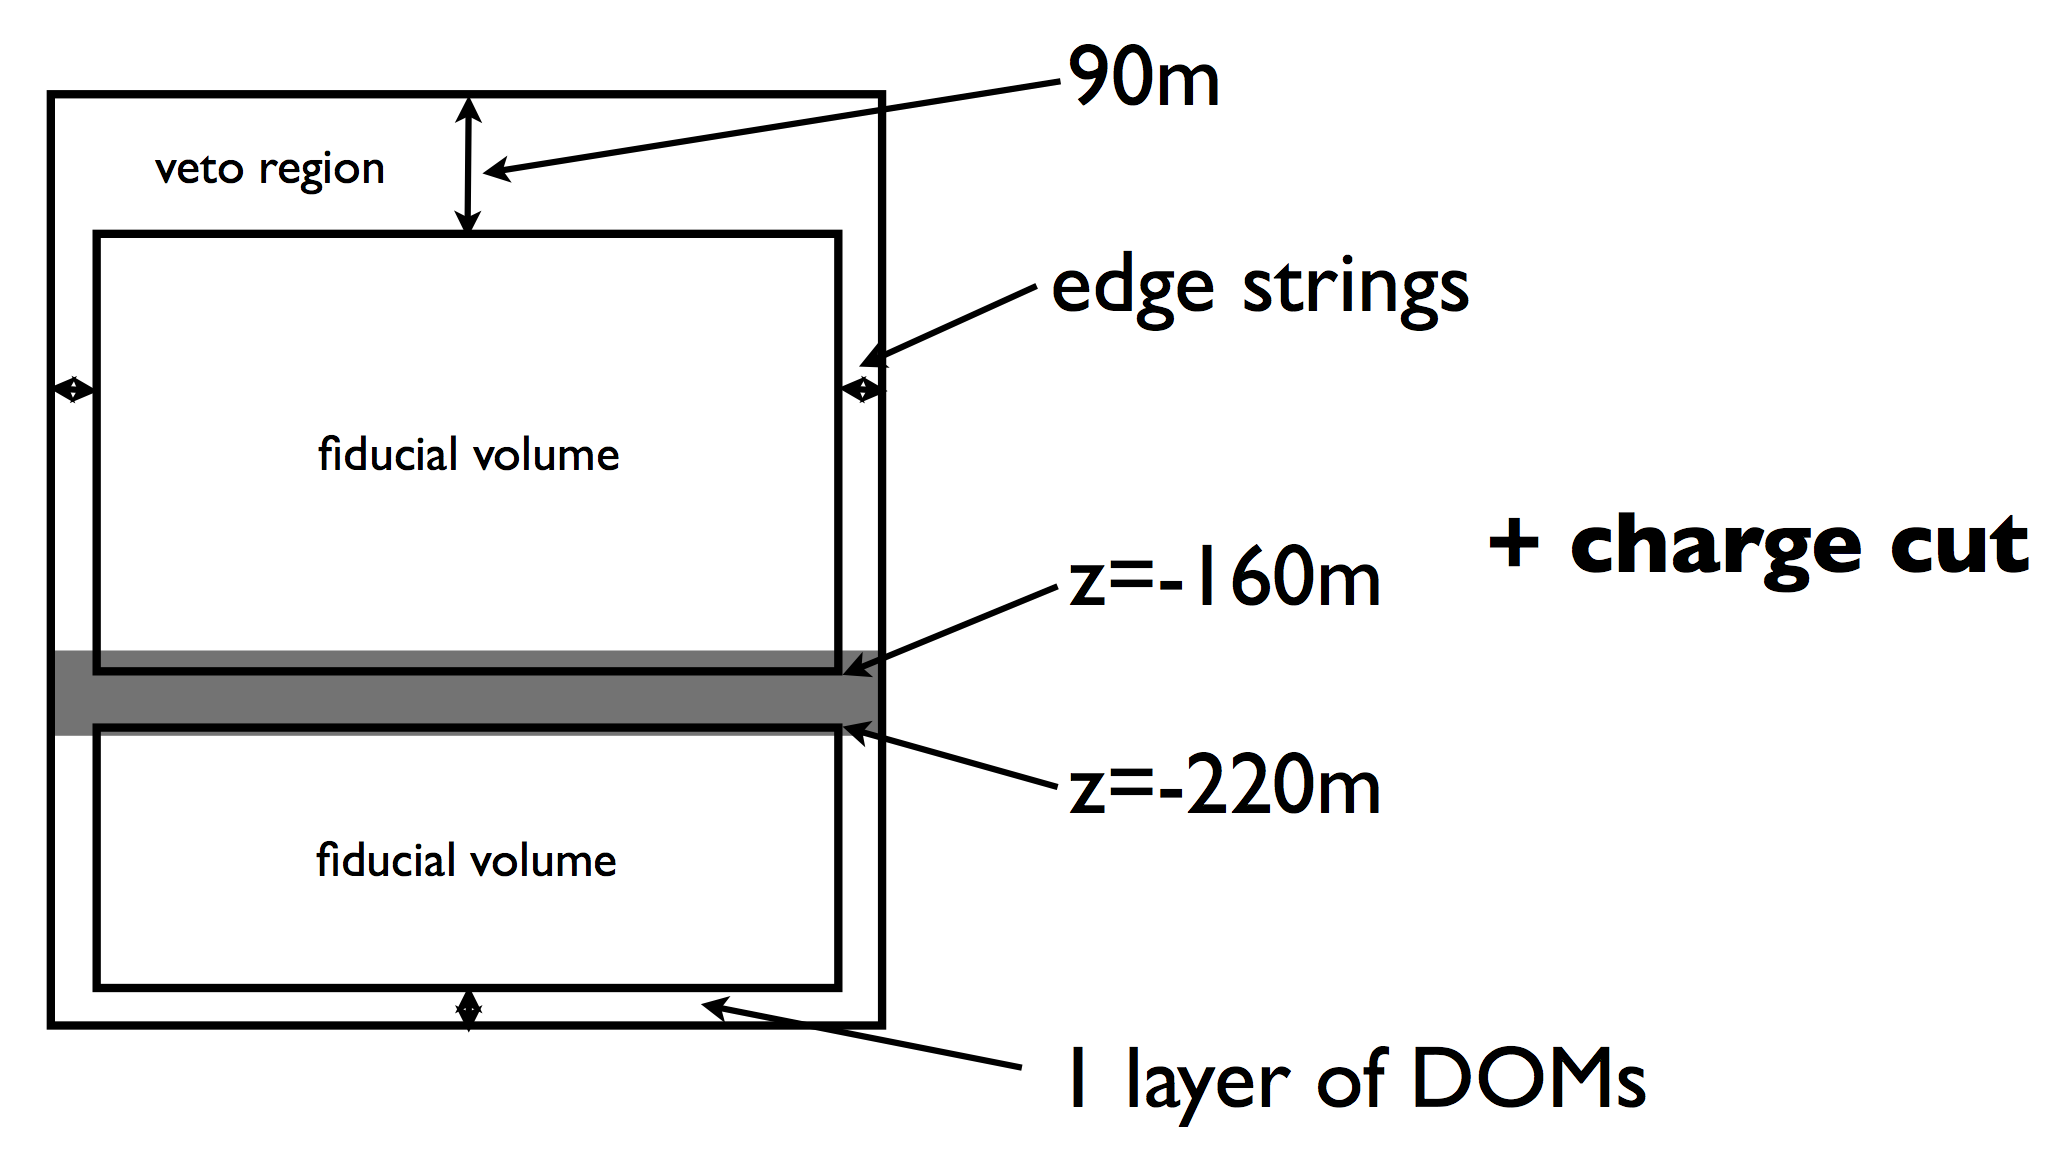
\includegraphics[width=0.5\linewidth]{figures/Fiducial_volume_full}}
	%\subfloat{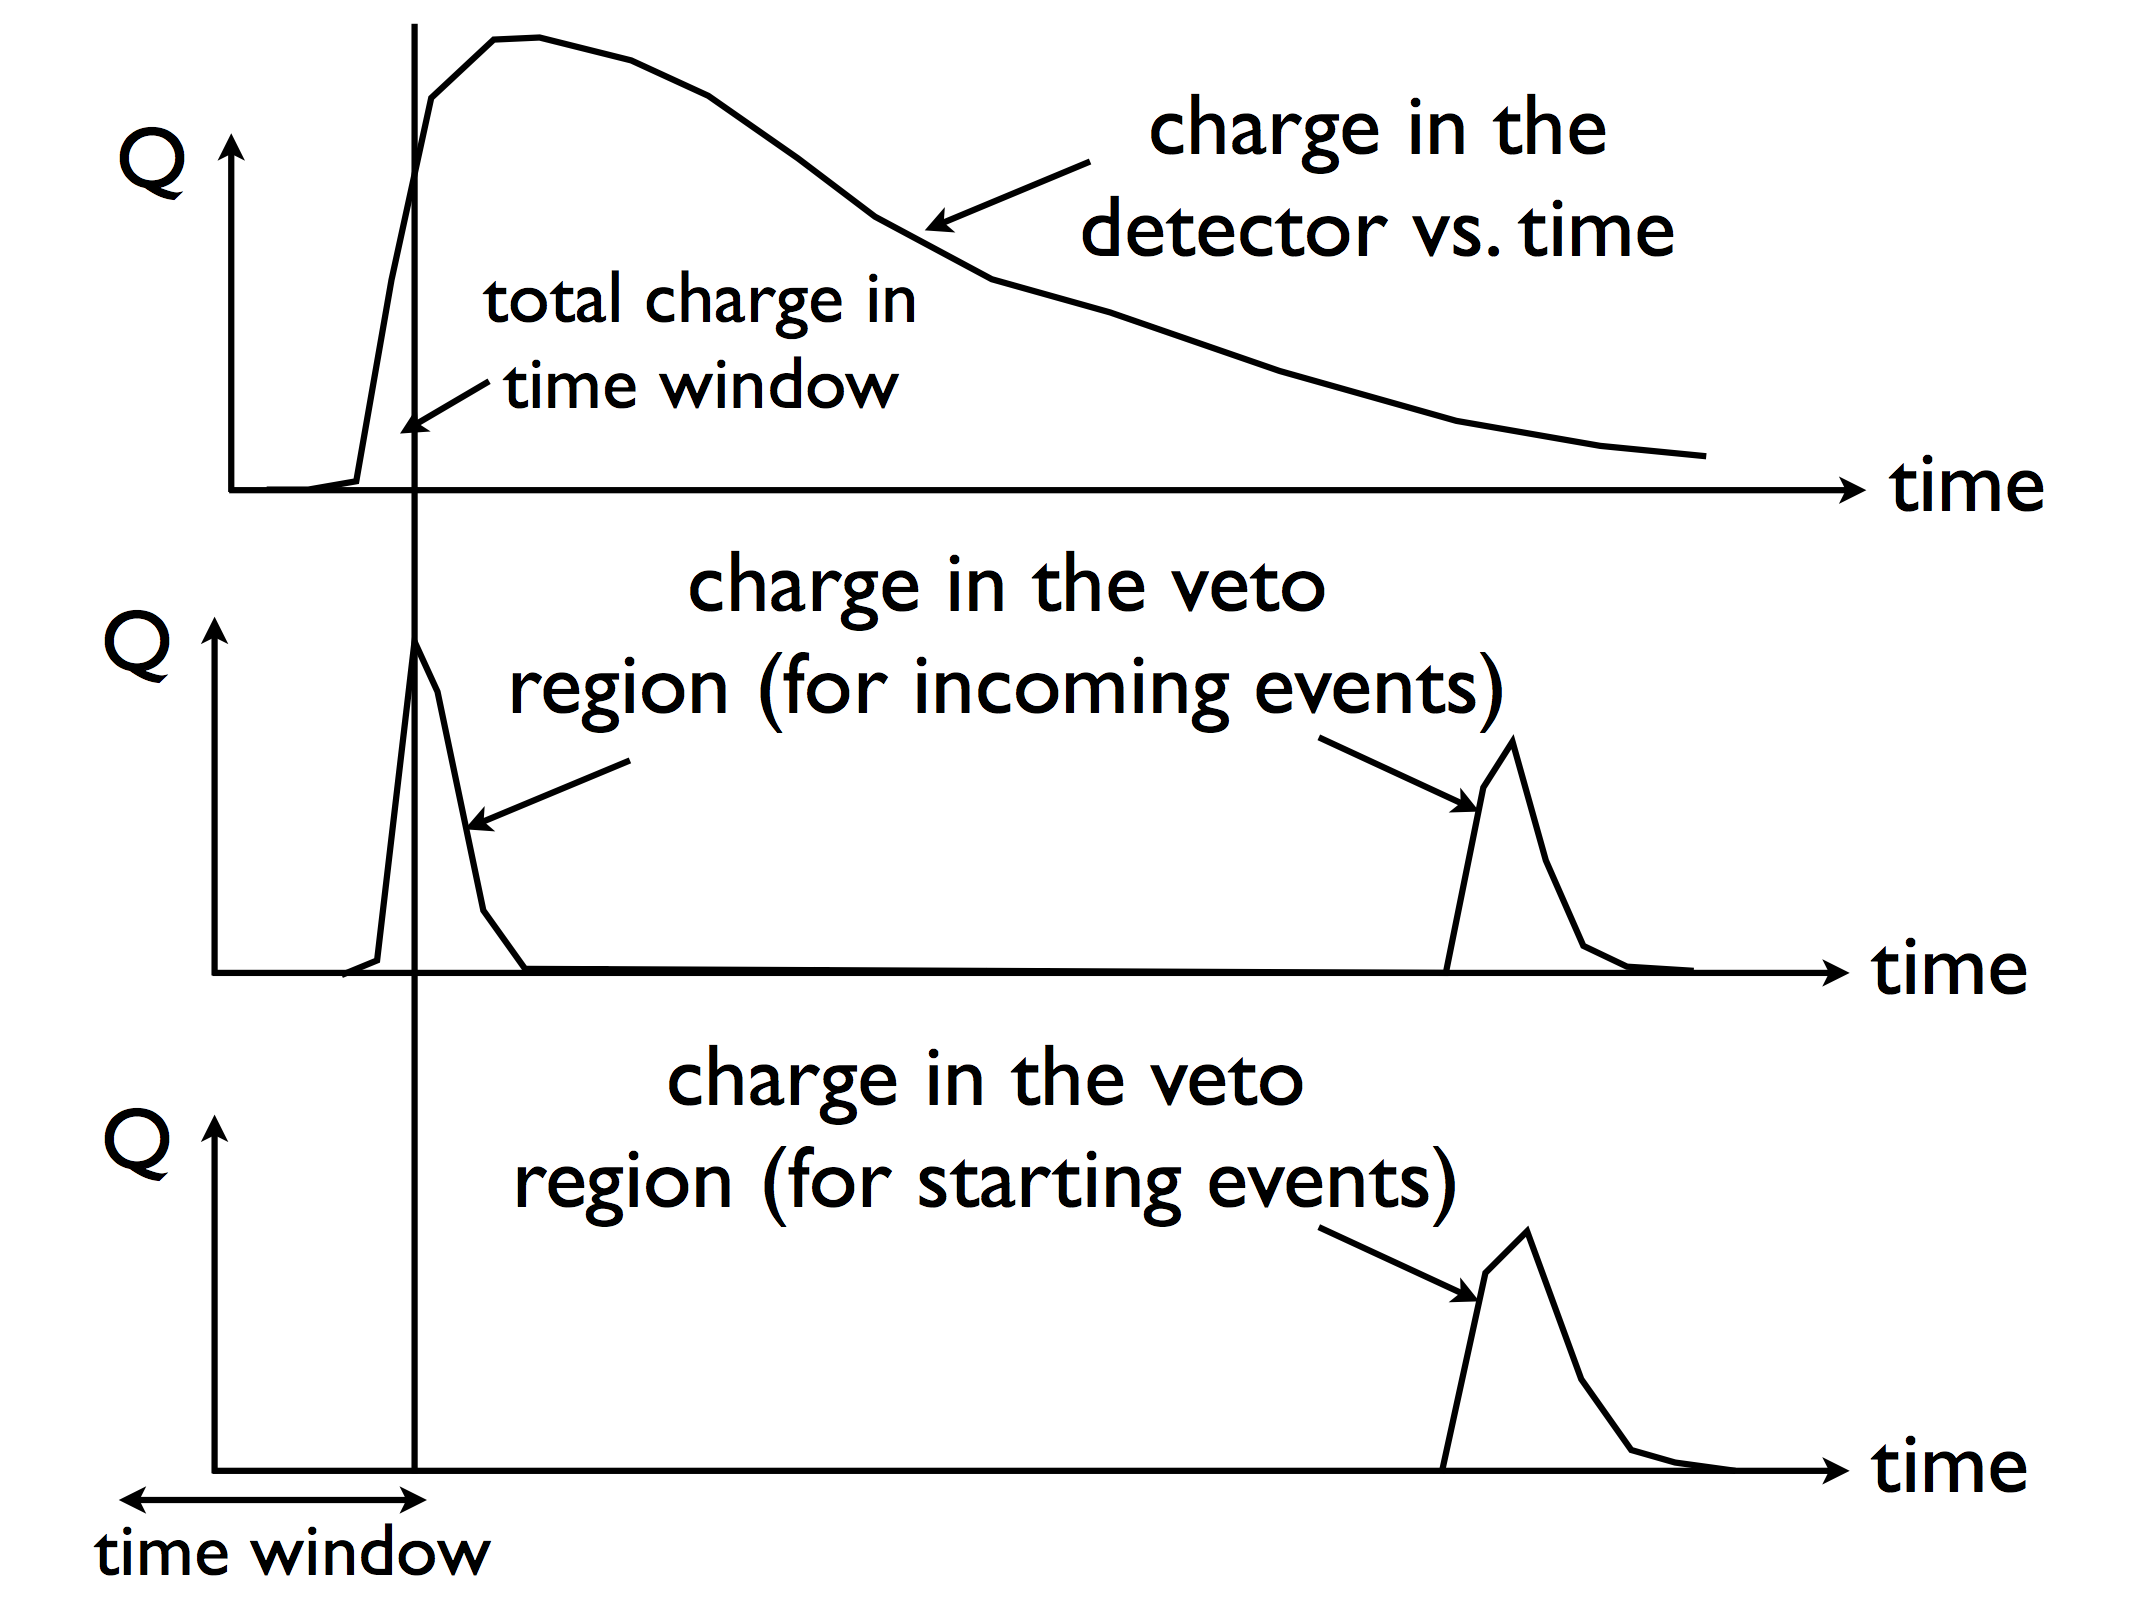
\includegraphics[width=0.4\linewidth]{figures/Charge_vs_time_with_veto_region}}
	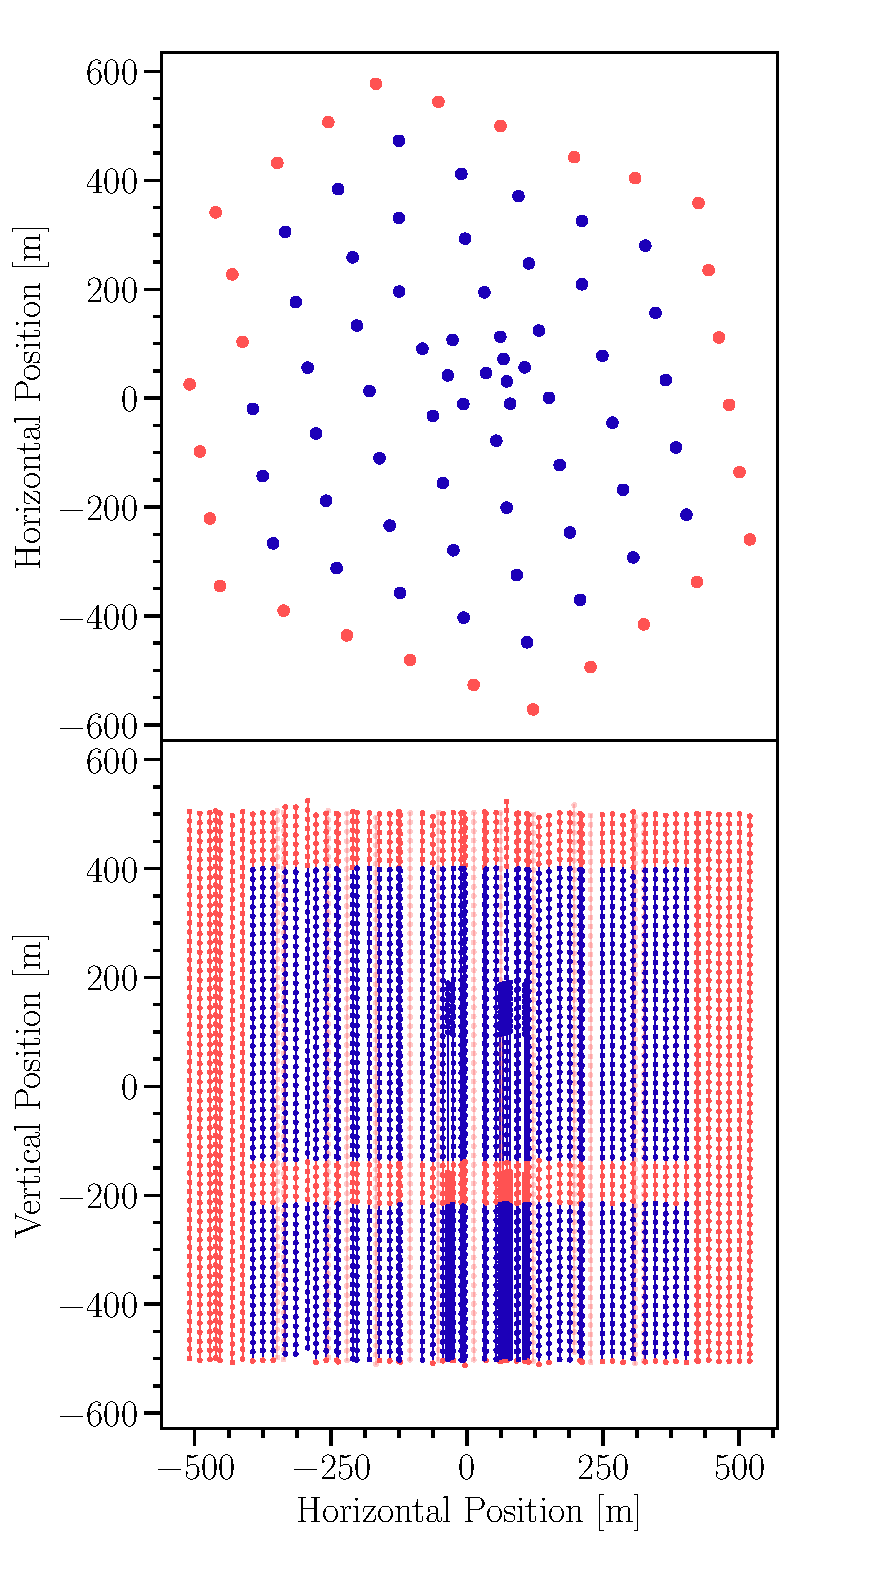
\includegraphics[width=\linewidth]{figures/hese_paper/veto_diagram_vertical}
	\internallinenumbers
	\caption{\textbf{\textit{HESE veto.}} Diagram of the IceCube detector with the veto DOMs indicated.
		Top panel: an overhead view of the IceCube detector.
		Positions of strings with only veto DOMs are shown in red, while those with at least one non-veto DOM are shown in blue.
		Bottom panel: a side view of the IceCube detector strings and DOMs.
		Veto DOMs are indicated with red circles, and non-veto DOMs with blue circles.
		Strings in front of or behind the region without veto-DOMs are semi-transparent.}\label{fig:veto}
\end{figure}

\begin{figure}
	\centering
	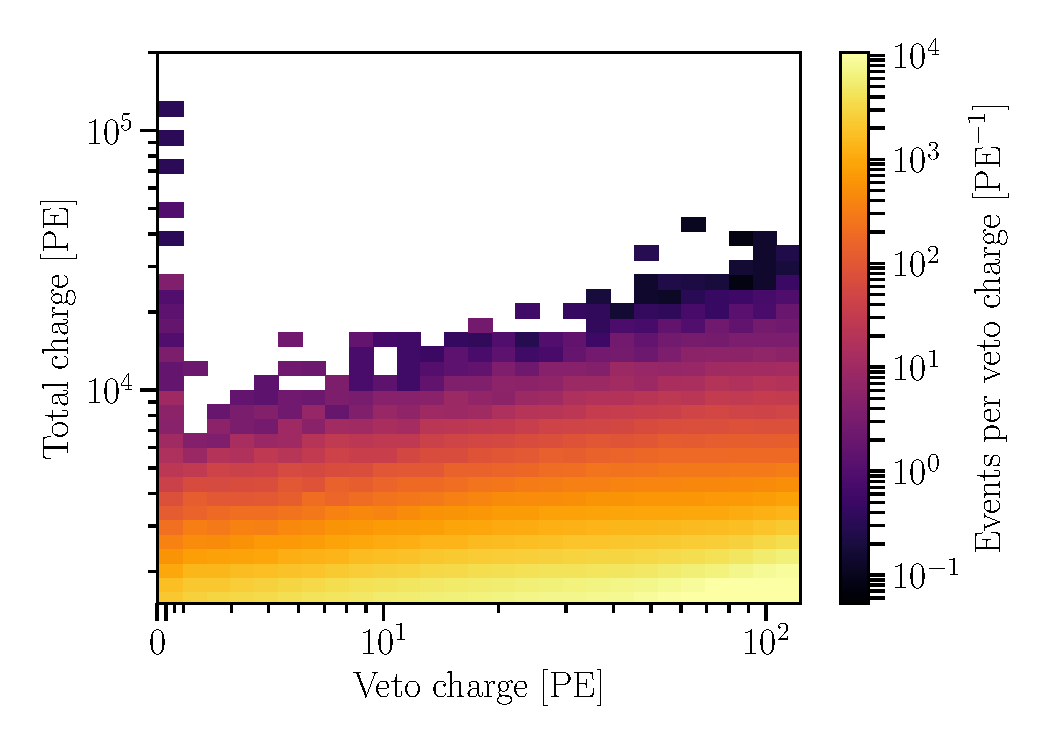
\includegraphics[width=\linewidth]{figures/hese_paper/veto_charge_plot}
	\internallinenumbers
	\caption{\textbf{\textit{Veto charge vs. total charge.}} The color scale shows the event density with respect to the veto charge, prior to the veto cuts and charge cuts, where darker color implies higher event density and lighter implies lower event density.
		The vertical axis is the total charge, in photo-electrons, deposited in the detector, while the horizontal axis is the veto charge as defined in \refsec{sec:selection}.
		The high-charge population of low-veto-charge events (between 0 and $\SI{3}\pe$) can be clearly seen against the background of higher-veto-charge events.}\label{fig:charge_veto}
\end{figure}

The high-energy starting-event (HESE) sample aims to isolate astrophysical neutrinos by reducing the background of not only atmospheric muons but also atmospheric neutrinos.
In order to do so, we make use of the outer parts of the detector as a veto layer and select only the events that deposit high charge in the detector and interact within the fiducial volume.
The fiducial volume approximately excludes the top-most $\SI{90}\meter$ of the detector, $\SI{90}\meter$ from the outer layer of DOMs on the detector sides, the bottom-most $\SI{10}\meter$ of DOMs, and a $\SI{60}\meter$ high horizontal layer of ice with the largest dust content.
The veto then consists of the DOMs excluded from the fiducial volume.
\reffig{fig:veto} shows a schematic of the veto.

To select events with their interaction vertex contained in the fiducial volume we must first define the approximate vertex time ($t_0$) and position ($\vec{x}_0$).
We define an event starting time when the integrated charge deposition in the detector reaches 250 photo electrons ($\si\pe$), excluding the DOMs in DeepCore, a higher density infill array, and considering only charges with hard-local-coincidence (HLC) triggers~\cite{Achterberg:2006md,Abbasi:2008aa,Aartsen:2016nxy}.
HLC triggered hits are DOM hits that are in coincidence ($\pm\SI{1}\mus$) with another hit on the four closest DOMs of the same string.
Choosing only HLC triggered hits reduces the noise and excluding DeepCore makes the detector response more uniform.
To further prevent random noise adding to the threshold over long time periods, a three microsecond time window is considered when computing the event start time.
This time window encompasses the duration of events expected to be seen by IceCube aside from monopole signatures~\cite{Lauber:2018ntx,Aartsen:2015exf,Aartsen:2014awd}.
The interaction vertex of the event is approximated by the charge-averaged position of the event's first $\SI{250}\pe$ from HLC hits.
To reduce the background of muons entering from outside the detector, we select only events with no more than three $\si\pe{}$s from veto hits and with veto hits on fewer than three DOMs.
We define a veto hit with time $t_1$ and position $\vec{x}_1$, in relation to the event vertex, as an HLC triggered hit that meets the conditions summarized in \reftab{tbl:veto_hits}.
The first condition is that the hit must be on a DOM within the veto region.
To select only hits from light originating outside the fiducial volume, we require veto hits to arrive before $t_0+\SI{50}\ns$; this cut is sufficient as the minimum distance from the fiducial volume to a veto DOM is $\SI{17}\meter$.
To reduce the contribution of noise, we require the time of veto hits to be within $\SI{3}\mus$ of the vertex time.
Finally, to select only hits that may be related to the event vertex, we require veto hits to be on DOMs within $\SI{3}\mus \cdot c$ ($\sim\SI{899}\meter$) of the event vertex position.
The $\SI{3}\pe$ veto cut removes atmospheric events that are likely to deposit charge in the veto region, but will not remove lower energy atmospheric events.
The distribution of data events with respect to veto charge and total charge is shown in \ref{fig:charge_veto}.
Atmospheric events comprise the bulk of the distribution above a veto charge of $\SI{3}\pe$, whereas below this threshold the distribution is dominated by a population of astrophysical neutrinos at higher total charge.

The definition of the veto has several advantages over non-veto methods~\cite{Niederhausen:2017mjk,Stettner:2019tok} in that it is designed to more robustly addresses uncertain muon and neutrino backgrounds, major obstacles to the measurement of the astrophysical flux.
%The definition of the veto has several advantages over non-veto methods~\cite{Niederhausen:2017mjk,Stettner:2019tok}.
Because there is a clear separation of the detector into fiducial volume and veto region, we can obtain a data driven estimate of the atmospheric muon background by using the outermost layer to identify muons, and performing the event selection in a reduced volume.
This method is described in more detail in~\refsec{sec:backgrounds}.
The event selection effective area is also approximately isotropic for astrophysical neutrinos (without accounting for absorption in the Earth), but the background has a highly zenith dependent acceptance.
This enables up/down asymmetry tests of the astrophysical flux in data.
In~\reftab{tbl:spl_bf_events_high} we can see that the background contamination from atmospheric muons is below $\SI{0.002}\percent$ of the events in the sample above $\SI{60}\TeV$.

To minimize the number of atmospheric events in the selection we make a strict charge cut, selecting only events with at least $\SI{6000}\pe$ deposited in the detector.
This cut was determined using burn-sample data, equivalent to $\SI{10}\percent$ of two years of detector operation, by requiring that no identified muons pass the charge cut.
This charge cut removes downward fluctuations in light yield, keeping only events that are high energy.
A charge cut is preferred over an energy cut, as it is more closely related to the observed event light yield and thus is a more robust estimator of expected veto charge.
For the analyses in~\refsec{sec:diffuse} we place a cut on the reconstructed deposited energy at $\SI{60}\TeV$ to further reduce muon contamination, as the shape and normalization of this background component is not well known.
The shape of the atmospheric muon and neutrino fluxes are closely related to each other, and bounded by the cosmic-ray flux so that they must be steeply falling.
The interaction of muons in the atmosphere and ice further softens the muon spectrum from that of cosmic rays.
Although there is uncertainty in the shape of the muon spectrum, the yield of muons from cosmic-ray air showers has more significant modelling uncertainties that stem from uncertainties in the hadronic interaction cross sections~\cite{Pierog:2017nes} and the cosmic-ray composition~\cite{Bluemer:2009zf}.
As we lack the capability to parameterize both the uncertainty in shape and normalization from first principles, we turn to data-driven techniques to constrain the size of this background.
Unfortunately, the data-driven techniques available do not provide us with enough events to determine the shape of the muon background.
For this reason we take a pragmatic approach to treat the muon component.
We use a simulation estimate of the muon flux shape which provides a reasonable estimate for a steeply falling muon spectrum, but neglects shape uncertainties.
The normalization is then constrained using tagged background in data, a procedure described in more detail in \refsec{sec:backgrounds}.
As we will see in \refsec{sec:backgrounds}, the muon component does not significantly contribute to the sample above $\SI{60}\TeV$.
The analyses in \refsec{sec:sources} do not impose the $\SI{60}\TeV$ cut as the analyses there conservatively assume that the data sample can be used to model the background distribution.

\begin{table}[t!]
	\centering
	\begin{tabular}{l}  % centered columns (2 columns)
		%\hline\hline                        %inserts double horizontal lines
		Veto-hit conditions \\ [0.5ex] % inserts table %heading
		\toprule                    % inserts single horizontal line
		1) Hit on DOM within veto region \\
		2) $t_1 \leq t_0+\SI{50}\ns$  \\
		3) $t_1 \geq t_0-\SI{3}\mus$  \\
		4) $\left|\vec{x}_0 - \vec{x}_1\right| \leq \SI{3}\mus \cdot c$ \\
		%[1ex]       % [1ex] adds vertical space
		%\hline     %inserts single line
	\end{tabular}
	\internallinenumbers
	\caption{\textbf{\textit{Summary of the veto-hit definition.}} Table contains the criteria a hit must satisfy to be considered a veto hit, where $t_0$ is the approximate vertex time and $\vec{x}_0$ is the approximate vertex position.
		If the veto hits constitute more than three photo-electrons or are distributed over more than two DOMs, the event is rejected from the sample.}\label{tbl:veto_hits}  % is used to refer this table in the text
\end{table}

\begin{table}[h!]
	\begin{minipage}{\linewidth}
		\begin{tabular}{l | c c | c}
			\toprule
			Category & $E < \SI{60}\TeV$ & $E > \SI{60}\TeV$ & Total \\
			\midrule
			Total Events & 42 & 60 & 102 \\
			\midrule
			Up	    & 19 & 21 & 40 \\
			Down	& 23 & 39 & 62 \\
			\midrule
			Cascade	& 30 & 41 & 71 \\
			Track	& 10 & 17 & 27 \\
			Double Cascade & 2 & 2 & 4 \\
			\bottomrule
		\end{tabular}
	\end{minipage}
	\begin{minipage}{\linewidth}
		\internallinenumbers
		\caption{\textbf{\textit{Observed events by category.}}
			The left-most column indicates the event category, which may correspond to a particular choice of morphology or direction.
			The right-most column shows the total number of data events observed in a given category.
			Intermediate columns split events into those with less than or greater than $\SI{60}\TeV$ reconstructed deposited energy.
		}
		\label{tbl:observed_events}
	\end{minipage}
\end{table}

\begin{table}[h!]
	\begin{minipage}{\linewidth}
		\begin{tabular}{l | c c c}
			\toprule
			Category & Cascade & Track & Double Cascades \\ 
			\midrule
			Total & $47.3$ & $12.6$ & $2.3$ \\ 
			\midrule
			$\nu_e$ & $\SI{58.8}\percent$ & $\SI{11.6}\percent$ & $\SI{23.1}\percent$ \\ 
			$\nu_\mu$ & $\SI{13.3}\percent$ & $\SI{76.2}\percent$ & $\SI{13.1}\percent$ \\ 
			$\nu_\tau$ & $\SI{27.8}\percent$ & $\SI{11.7}\percent$ & $\SI{63.8}\percent$ \\ 
			\midrule
			$\nu_e$ CC & $\SI{54.4}\percent$ & $\SI{10.6}\percent$ & $\SI{20.5}\percent$ \\ 
			$\nu_\mu$ CC & $\SI{7.4}\percent$ & $\SI{74.9}\percent$ & $\SI{10.1}\percent$ \\ 
			$\nu_\tau$ CC & $\SI{24.1}\percent$ & $\SI{11.0}\percent$ & $\SI{62.0}\percent$ \\ 
			\midrule
			CC & $\SI{85.9}\percent$ & $\SI{96.5}\percent$ & $\SI{92.6}\percent$ \\ 
			NC & $\SI{13.4}\percent$ & $\SI{2.8}\percent$ & $\SI{6.5}\percent$ \\
			\bottomrule
		\end{tabular}
	\end{minipage}
	\begin{minipage}{\linewidth}
		\internallinenumbers
		\caption{\textbf{\textit{Expected events by category for best-fit parameters above $\SI{60}\TeV$.}} Each row specifies a particle type or interaction type. Here, CC stands for deep inelastic charged-current scattering and NC its neutral-current counterpart. Each column specifies the morphology, where percentages are computed with respect to the total number of expected events at the top of the column. The percentages have been rounded to one decimal point.}
		\label{tbl:misid}
	\end{minipage}
\end{table}


In \reftab{tbl:observed_events} we list the number of observed events that pass the above criteria -- which we summarize in \reftab{tbl:hese_cuts} -- from seven and a half years of observation, corresponding to a livetime of 2635 days.
%%AK: I think we should add a 1 D histogram of  the energy distribution
% Maybe put in a 1D charge histogram since we are talking about charge and have not introduced the veto yet
A total of 102 events were observed: 27 tracks, 71 cascades, and 4 double cascades.
Even though the event selection has not changed with respect to previously reported results~\cite{Aartsen:2013jdh,Aartsen:2014gkd,Aartsen:2015zva,Aartsen:2017mau} the event properties and the selected events themselves have changed due to an overall detector re-calibration.
The net effect of this re-calibration is a decrease of total observed charge, which results in some events dropping below the total charge cut.
Due to this re-calibration eight events were dropped from the sample.
%%AK: how much did the energy of eg, Bert and Ernie change? May need to be more quantitative than this
% and explain what was done, few sentences.
% Make a plot of the charge distribution before and after the re-calibration
% Maybe explicitly reference the changes for a few events
Seven events were removed by the charge cut: four cascades and three tracks.
Of these, only three -- one cascade and two tracks -- had deposited energy above $\SI{60}\TeV$ where the measurements of the astrophysical component are performed; see \refsec{sec:diffuse}.
An additional track event was also removed as it now fails the veto criterion: the hits in causal connection to the start of the events have increased due a modification of the event's start time.

The two double cascades above $\SI{60}\TeV$ have a high probability of originating from $\nu_\tau$ charged-current interactions, while the two below $\SI{60}\TeV$ are in a region with higher contamination from other neutrino flavors and larger background uncertainties.

\begin{table}[t!]
	\centering
	\begin{tabular}{l r}  % centered columns (2 columns)
		%\hline\hline                        %inserts double horizontal lines
		Parameter & Cut value \\ [0.5ex] % inserts table %heading
		\toprule                    % inserts single horizontal line
		Event start time charge threshold & 250 PE  \\
		Maximum charge in veto region & 3 PE  \\
		Maximum DOMs with veto hits & 2 \\
		Minimum total charge & 6000 PE  \\
		Vertex time window & 3 $\mu s$  \\
		%[1ex]       % [1ex] adds vertical space
		%\hline     %inserts single line
	\end{tabular}
	\internallinenumbers
	\caption{\textbf{\textit{Summary of the HESE cuts and definitions.}} Table contains the cuts and thresholds of the HESE analysis.
		PE stands for photo-electron.}\label{tbl:hese_cuts}  % is used to refer this table in the text
\end{table}


\section{Reconstruction and simulation}

Reconstruction of the neutrino events involves determining the interaction vertex, the incident direction, and the energy depositions -- positions and magnitudes -- in the detector.
The interaction vertex determined as discussed in \refsec{sec:selection} is used only in the event selection cuts, while the more sophisticated reconstructions described in this section introduce the interaction vertex as a free parameter.

To reconstruct events, we separately consider hypotheses formed according to the three morphologies: track, cascade, and double cascade.
For each of these hypotheses we determine the expected light arrival time distribution on all DOMs, and maximize the likelihood of these light distributions given the data with respect to the direction, vertex, and energy depositions as described in~\cite{Aartsen:2013vja}.

To incorporate information about the flavor of neutrinos in the sample, we assign each event a reconstructed morphology according to the classification algorithm described in~\cite{Usner2018Search}.
This algorithm can be broken into five distinct steps.
One, a series of quality cuts are made on the output of the double cascade reconstruction, namely the double cascade reconstruction must not fail and the opening angle between the track and double cascade reconstructions must be less than or equal to $\SI{30}\degree$.
Two, if the quality cuts fail, the likelihood of the reconstructed cascade and track directions are compared to assign the morphology as cascade or track.
Three, if the quality cuts pass, events with reconstructed length $L < \SI{10}\meter$ are assigned the cascade morphology.
Four, remaining events with energy confinement $E_C < 0.99$ are assigned the track morphology.
To define the energy confinement we first define the energy of each cascade within $\SI{40}\meter$ as $E_{1,C}$ and $E_{2,C}$.
Then the confinement is given by $E_C = (E_{1,C} + E_{2,C}) / E_{\textmd{tot}}$, where $E_\textmd{tot}$ is the total reconstructed energy of the event.
Five, remaining events with energy asymmetry $-0.98 \leq E_A \leq 0.3$ are assigned the double cascade morphology, other remaining events are assigned the cascade morphology.
The energy asymmetry is the ratio of the difference between the two double cascade reconstructed energy depositions and the sum of the two energy depositions, $E_A = (E_1 - E_2)/(E_1 + E_2)$, where $E_1$ and $E_2$ are the reconstructed energy of each cascade.
This method produces a high-purity selection of tau neutrinos in the double cascade category above $\SI{60}\TeV$, and discriminates well between true cascades and true tracks, but there remain contributions from all flavors in all three morphological categories which are outlined in \reftab{tbl:misid}.
Despite the non-negligible rate of mis-identification, the asymmetry in the contributions can be used to constrain the flavor composition of the neutrino events.

The magnitude of energy depositions in the detector can be reconstructed to high accuracy if they are contained within the detector.
In this sample the median deposited energy resolution is $\sim\SI{7.9}\percent$, $\sim\SI{11}\percent$, and $\sim\SI{7.81}\percent$ for reconstructed cascades, tracks, and double cascades respectively.
\reffig{fig:energy_resolution} shows the median deposited energy resolution as a function of deposited energy for the three reconstructed morphologies.
Some of the reconstruction uncertainty comes from the differences in light yield for electromagnetic and hadronic showers, particularly for cascades of which $\sim\SI{15}\percent$ are NC events; see \reftab{tbl:misid} for more details.
The deposited energy is correlated with the neutrino energy, and so can be used to constrain the neutrino energy spectrum.
However, the kinematics of the neutrino interactions can result in small estimated deposited energy compared to the energy of the neutrino.
The left panel of \reffig{fig:transfer_matrices} shows this correlation, where the deposited energy is peaked close to the neutrino energy, as well as the long tails of the reconstructed distribution.
To visualize this more clearly, \reffig{fig:energy_spread} shows the distribution of reconstructed deposited energy for slices in true neutrino energy, where the selection truncates the tail of the distribution for lower neutrino energies.
If we na\"ively use the deposited energy as a proxy for the neutrino energy, then we obtain a median neutrino energy resolution of $\sim\SI{11}\percent$, $\sim\SI{30}\percent$, and $\SI{18}\percent$ for reconstructed cascades, tracks, and double cascades respectively.

The angular reconstruction is more straightforward by comparison, as the angle between the primary neutrino and secondary particles of the interaction is negligible compared to reconstruction uncertainties at the energy scale we are concerned with.
The analyses described in \refsec{sec:diffuse} do not use the azimuthal directional information.
Cascades, tracks and, double cascades in this sample have a median azimuthal resolution of $\sim\SI{6.8}\degree$, $\sim\SI{1.8}\degree$, and $\sim\SI{5.6}\degree$ respectively.
The inter-DOM spacing is smallest along the vertical axis and so the zenith resolution will in general be better than the azimuthal resolution.
Cascades, tracks, and, double cascades in this sample have a median zenith resolution of $\sim\SI{6.26}\degree$, $\sim\SI{1.46}\degree$, and $\sim\SI{4.98}\degree$ respectively.
The track angular resolution in this sample is worse than the resolution in $\nu_\mu$ dominated samples~\cite{Stettner:2019tok} due to the non-negligible contamination from $\nu_e$ and $\nu_\tau$; see \reftab{tbl:misid} for details.
The angular resolution of cascades is limited by the resolution of photon arrival times, interaction vertex, and our modelling of photon propagation in ice~\cite{Aartsen:2013rt,Aartsen:2016nxy}.
We can explain the better angular resolution of tracks and double cascades by considering the longer path length of the highly-boosted secondary lepton.
The energy depositions of this lepton produce detector hits further away in space and time from the neutrino interaction vertex, placing more stringent restrictions on both the timing of the event and its path through the detector.
This behavior in turn limits the viable directions when reconstructing the event and leads to better angular resolution for tracks.
To summarize the behavior of the angular reconstruction, the right panel of \reffig{fig:transfer_matrices} shows the distribution of reconstructed zenith angles as a function of the true neutrino zenith angle.
The large smearing in this matrix arises from the cascades that dominate the data sample.

\begin{figure}
	\centering
	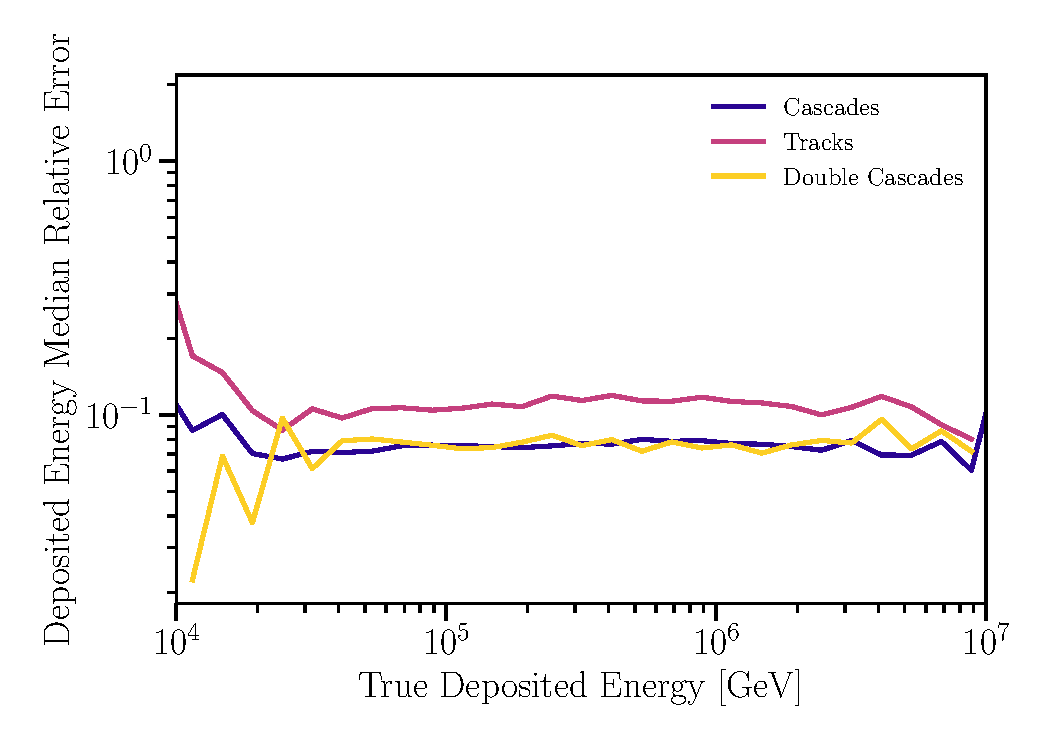
\includegraphics[width=\linewidth]{figures/hese_paper/energy_resolution}
	\internallinenumbers
	\caption{\textbf{\textit{Deposited energy resolution.}} Plotted as a function of the true deposited energy in the detector, each line shows the median energy resolution for a reconstructed morphology.
		At these energies the uncertainty is dominated by uncertainties in the direction and interaction vertex.
	}\label{fig:energy_resolution}
\end{figure}

\begin{figure*}
	\centering
	\subfloat{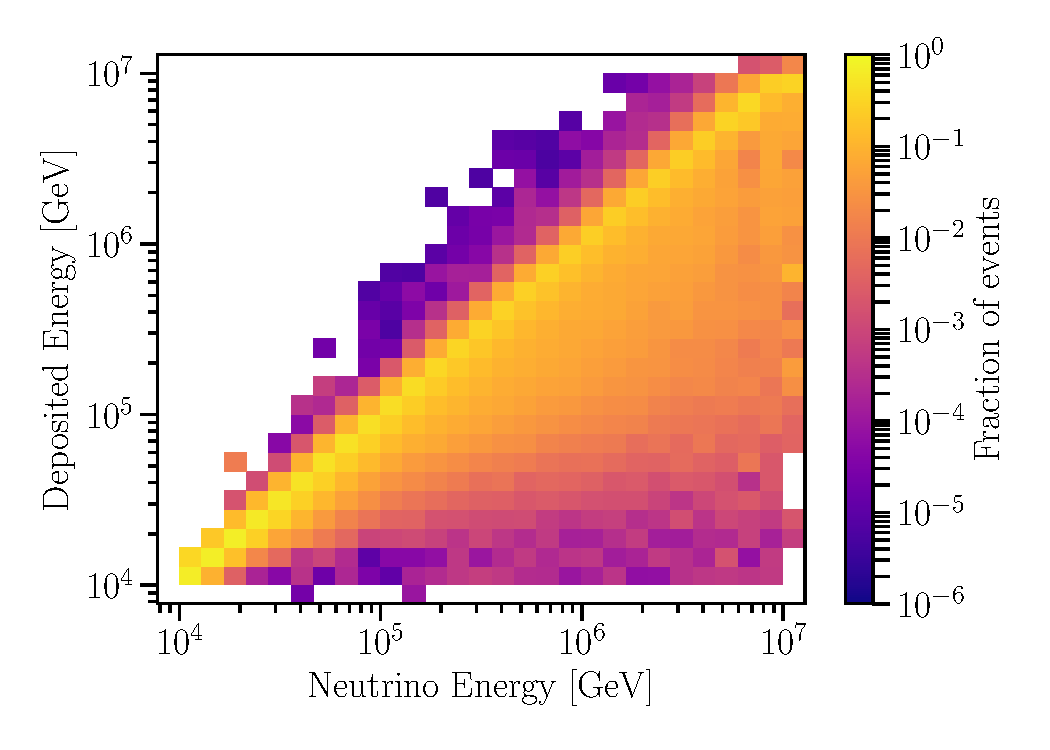
\includegraphics[width=0.5\linewidth]{figures/hese_paper/energy_transfer_matrix_all}}
	\subfloat{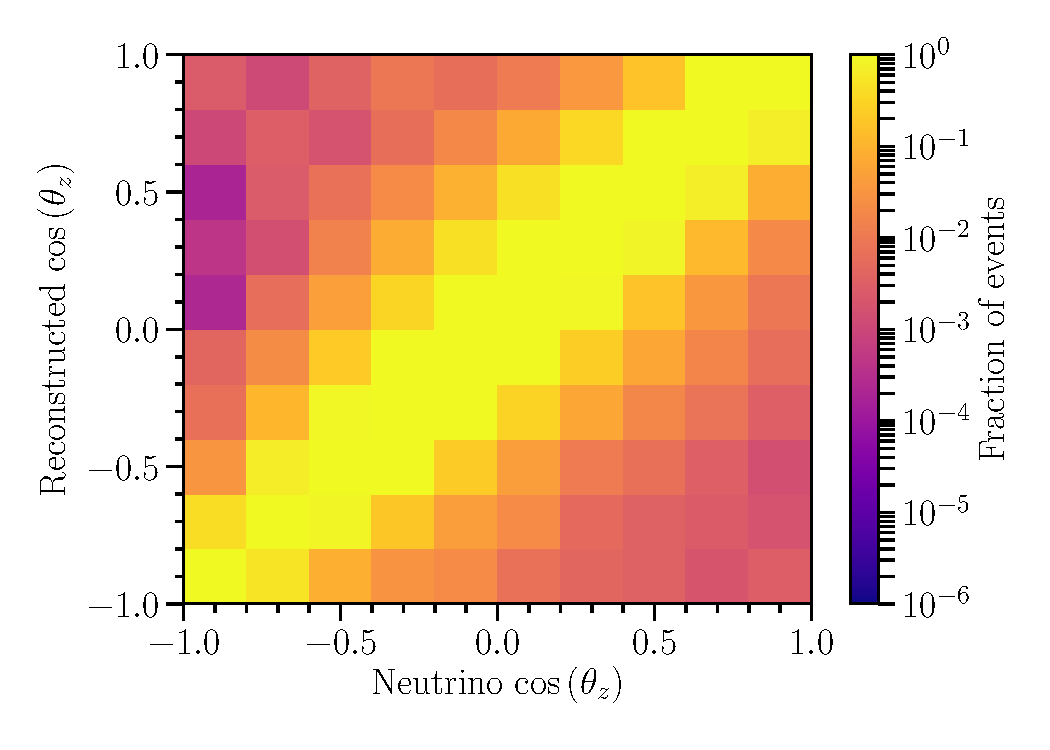
\includegraphics[width=0.5\linewidth]{figures/hese_paper/zenith_transfer_matrix_all_all}}
	\internallinenumbers
	\caption{\textbf{\textit{Distribution of expected reconstruction quantities as a function of true parameters.}} Transfer matrices, evaluated at the MC best-fit parameters, are shown for all morphologies combined.
		The probability of a reconstructed deposited energy for a given neutrino energy (left) and the probability of a reconstructed cosine of the zenith angle for a particular cosine of the neutrino zenith angle (right) are shown.
		The matrices are column normalized.}\label{fig:transfer_matrices}
\end{figure*}

\begin{figure}
	\centering
	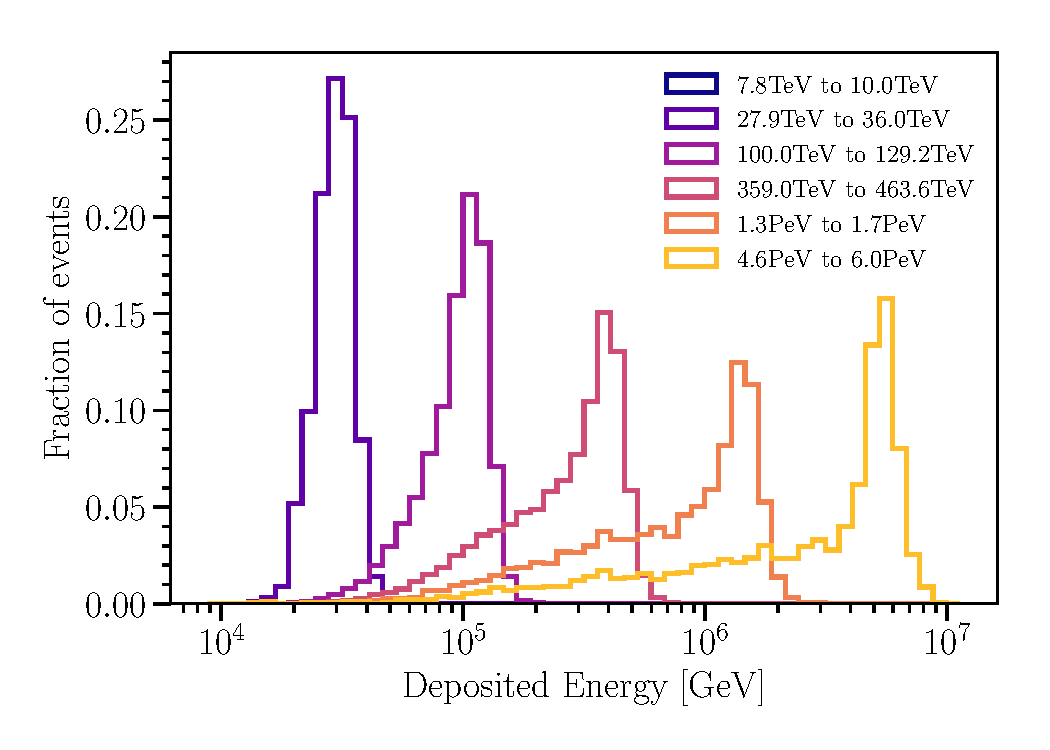
\includegraphics[width=\linewidth]{figures/hese_paper/deposited_energy_fine_distribution_all_energiesallall}
	\internallinenumbers
	\caption{\textbf{\textit{Deposited energy probability distributions.}} Probability distribution of reconstructed deposited energies for slices of true neutrino energy for all morphologies weighted to the best-fit parameters}\label{fig:energy_spread}
\end{figure}

% Scatter plot of E_dep vs cos(theta)
\begin{figure}
	\centering
	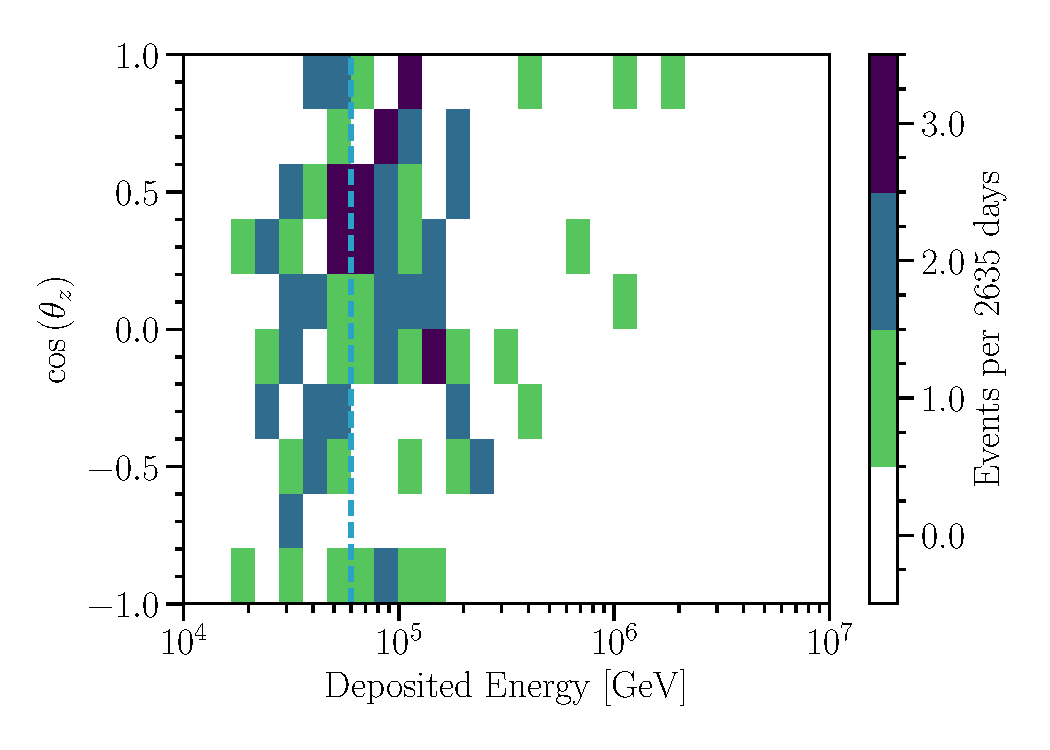
\includegraphics[width=\linewidth]{figures/hese_paper/diffuse_hist_all_data}
	\internallinenumbers
	\caption{\textbf{\textit{HESE events observed in $\SI{7.5}\year$.}} Histogram of the observed events as a function of their inferred deposited energy and cosine of the reconstructed zenith angle.
		The dashed line indicates the low-energy threshold of $\SI{60}\TeV$.}\label{fig:hese_events}
\end{figure}

The reconstruction method used in the analyses described in \refsec{sec:diffuse} have been changed to improve the accuracy of the analysis in several ways compared to previous analyses~\cite{Aartsen:2013jdh,Aartsen:2014gkd,Aartsen:2015zva,Aartsen:2017mau}.
A minimizer is now used for directional reconstruction, as opposed to the progressively narrower brute-force scans of the neutrino direction previously used.
The morphology determination is now performed algorithmically, whereas previous analyses performed morphology identification by hand.
These improvements make it feasible to run the reconstruction and classification on simulation events.
As a direct result of this, we now account for reconstruction and classification uncertainties on an event-by-event basis, as opposed to using average reconstruction and classification uncertainties.
Finally, the third morphology type (double cascades) is now included, as opposed to only tracks and cascades.
These improvements incorporate additional flavor information into the fit and result in a more accurate estimation of the expected event rates and distributions.

In the search for neutrino sources, a conservative choice is made to model the atmospheric background with data-derived distributions in an effort to avoid potential bias from mismodelling of the atmospheric backgrounds.
For a sample of such high signal purity, this method is only sensitive to a high degree of spatial clustering.
As MC is not used in this approach, we are able to use a more accurate but computationally more expensive directional reconstruction for the analyses outlined in \refsec{sec:sources}, that would otherwise be prohibitive to use on a MC sample.
Events in data are reconstructed by fully re-simulating cascades or tracks with in-ice photon propagation~\cite{Chirkin:2013dfi}.
To summarize here, first a localized random search steps through a five-dimensional parameter space that describes the interaction vertex and event direction.
Through this process we attempt to find the minimum of the test-statistic described in~\cite{Chirkin:2013lya} by comparing re-simulated waveforms to data.
At each step, the test-statistic is minimized with respect to the energy and time of the event.
Next, an ``approximate Bayesian calculation''~\cite{Marjoram15324} is performed around the estimated minimum using the same test-statistic in order to sample the posterior distribution of the vertex and direction; assuming a uniform prior in direction and vertex position.
This method allows us to sample from a posterior distribution without needing a proper likelihood that can be deterministically evaluated.
Marginalizing over the interaction vertex gives the posterior of the direction. The directional posterior distribution is parameterized  by an eight-parameter Fisher-Bingham distribution, which is used in \refsec{sec:sources}.
The errors reported for these events are notably larger than those quoted previously for the same events.
This stems from the different treatment of uncertainties.
Previously, re-simulations of the events used variations of the scattering and absorption for individual ice layers, but neglected other uncertainties.
Whereas the reconstruction now used for the source searches explicitly includes calibration uncertainty on the simulated light yield.
This change in the treatment of uncertainty results in larger errors which are consistent with other treatments of the calibration uncertainty~\cite{Aartsen:2019jcj}.
As such, the previously reported errors were likely underestimated.

With the exception of four events classified as double cascades, data are reconstructed based on the classification described above.
The four double cascades are reconstructed assuming a cascade hypothesis for the source searches.

\section{Determination of atmospheric neutrino and muon backgrounds\label{sec:backgrounds}}

The backgrounds in measuring the astrophysical neutrino flux are atmospheric neutrinos and muons.
Atmospheric neutrinos are predominantly produced by the decay of pions and kaons, which we shall call the ``conventional'' component.
At energies above $\SI{1}\TeV$ the spectrum of the conventional component is softer than the incident cosmic-ray spectrum by one unit in the spectral index, due to the interactions of these mesons in the atmosphere, and it is peaked at the horizon, $\cos\theta_z=0$~\cite{Gaisser:2002jj,Barr:2004br,Honda:2006qj,Petrova:2012qf}.
A sub-leading -- yet unobserved -- contribution due to charmed hadron decays is expected to be important above $\sim\SI{100}\TeV$~\cite{Bhattacharya:2015jpa}.
Since the charmed hadrons decay promptly and do not interact in the atmosphere at the energies relevant for this analysis, we call this the ``prompt'' component.
Thus, at these energies, the prompt component has a spectral index close to the incident cosmic-ray spectrum and is constant with respect to the cosine of the zenith angle.
The angular and energy distribution of the initial atmospheric neutrino flux is modified since the Earth is not transparent to neutrinos at these energies.
We account for this using a dedicated Monte Carlo, similar to the one described in~\cite{Gazizov:2004va}.
In this Monte Carlo we use the isoscalar neutrino cross sections given in~\cite{CooperSarkar:2011pa} for the neutrino-nucleon interactions.
Neutrino-electron scattering can be safely neglected except for resonant-W production~\cite{Glashow:1960zz} which we include.
We ignore the uncertainties on the Earth opacity as they are known to be sub-leading in this energy range~\cite{Gandhi:1995tf,CooperSarkar:2011pa,Vincent:2017svp}.
In order to account for uncertainties in the cosmic-ray flux~\cite{Dembinski:2017zsh} and hadronic interactions~\cite{Fedynitch:2012fs} we parameterize the atmospheric neutrino flux as
\noindent
\begin{linenomath*}
	\begin{equation}
	\begin{split}
	\phi_\nu^{\textrm{atm}} =& \Phi_{conv} \bigg(\phi^\pi_\nu + R_{K/\pi} \phi^K_\nu\bigg) {\bigg(\frac{E_\nu}{E_0^c} \bigg)}^{-\Delta \gamma_{CR}} \\ &+ \Phi_{prompt} \phi^p_\nu {\bigg(\frac{E_\nu}{E_0^p} \bigg)}^{-\Delta \gamma_{CR}},
	\end{split}
	\label{eq:atm_flux_equation}
	\end{equation}
\end{linenomath*}
where $\phi^\pi_\nu$, $\phi^K_\nu$, and $\phi^p_\nu$ are the conventional pion, kaon, and prompt atmospheric neutrino fluxes at a neutrino energy $E_\nu$ respectively as given in the Honda {\it{}et al.} and BERSS flux calculations~\cite{Honda:2006qj,Bhattacharya:2015jpa}
\footnote{For our conventional component we use the parameterization of~\cite{Honda:2006qj} given in~\cite{Montaruli:2011as}, which at the highest energies uses the parameterization in~\cite{Gaisser:2002jj}.
	This does not account for the contribution of $K_s$~\cite{Gaisser:2014pda}, which is $\sim \SI{10}\percent$ at $\SI{100}\TeV$ and well-within our uncertainties see Sec.~\ref{sec:systematics}};
the parameters $\convnorm$ and $\promptnorm$ account for uncertainties in the conventional and prompt normalizations respectively; $\pik$ allows us to modify the relative kaon to pion contributions; and the $\crdeltagamma$ parameter allows for hardening or softening of the atmospheric neutrino component to account for uncertainties in the cosmic-ray flux slope.
These parameters are incorporated into the analysis as nuisance parameters with priors as summarized in \reftab{tbl:priors}.
This analysis refrains from using prior information from other IceCube studies in order to provide independent results.
The conventional normalization prior width is motivated by studies of the total uncertainty due to cosmic-ray and high-energy hadronic processes~\cite{Fedynitch:2012fs}.
The width of the cosmic-ray slope parameter has been chosen to be $0.05$ in order to accommodate values measured at intermediate~\cite{Karelin:2011zz} and high~\cite{Bartoli:2015fhw,Yoon:2017qjx,Alfaro:2017cwx} energies.
The ratio of neutrinos-to-anti-neutrinos and pion-to-kaon yields uncertainty was estimated by comparing the expectation of different atmospheric neutrino calculations and picking a width that encompasses their prediction; see~\cite{CollinFluxes,Jones:2015bya} for details.
The prior on the atmospheric muon rate reflects the statistical uncertainty on our muon background tagging measurement, and is chosen conservatively.
The detector efficiency parameters uncertainties have been found by studying dedicated flasher data and low-energy muons~\cite{Aartsen:2016nxy}.
Finally, the parameters $E_0^c=\SI{2020}\GeV$ and $E_0^p=\SI{7887}\GeV$ are points of fixed differential flux chosen to be close to the median of the conventional and prompt flux event distributions.

% Table of all systematics and their priors if applicable
\begin{table*}[thb]
	\centering
	% systematic parameter & prior type & mean & sigma & min & max
	\begin{minipage}{\linewidth}
		\begin{tabular}{l rrr}
			%\toprule
			%& \multicolumn{5}{c}{Prior information} \\
			%\cmidrule{2-6}
			Parameter & Prior (constraint) & Range & Description \\
			\toprule
			\multicolumn{1}{l }{\textbf{Astrophysical neutrino flux:}} & & & \\
			$\astronorm$ & - & $[0,\infty)$ & Normalization scale\\
			$\astrodeltagamma$ & - &  $(-\infty,\infty)$ & Spectral index\\
			%$\theta_a$ & Uniform &  &  & 0 & 1 \\ \hline
			%$\theta_b$ & Uniform &  &  & -1 & 1 \\ \hline
			%${2\nu/\left(\nu+\bar{\nu}\right)}_\texttt{astro}$ & - & $[0,2]$\\
			&&\\
			\midrule
			\multicolumn{1}{l }{\textbf{Atmospheric neutrino flux:}} & & &\\
			$\convnorm$ & $1.0\pm0.4$ & $[0, \infty)$ & Conventional normalization scale\\
			$\promptnorm$ & - & $[0, \infty)$ & Prompt normalization scale\\
			$\pik$ & $1.0\pm0.1$ & $[0, \infty)$ & Kaon-Pion ratio correction\\
			$\atmonunubar$ & $1.0\pm0.1$ & $[0,2]$ & Neutrino-anti-neutrino ratio correction\\
			&&\\
			\midrule
			\multicolumn{1}{l }{\textbf{Cosmic ray flux:}} & & &\\
			$\crdeltagamma$ & $0.0\pm 0.05$ & $(-\infty,\infty)$ & Cosmic-ray spectral index\\
			$\muonnorm$ & $1.0\pm 0.5$ & $[0,\infty)$ & Muon normalization scale\\
			&&\\
			\midrule
			\multicolumn{1}{l }{\textbf{Detector:}} & & &\\
			$\domeff$ & $0.99 \pm 0.1$ & $[0.80, 1.25]$ & Absolute energy scale\\
			$\holeice$ & $0.0 \pm 0.5$ & $[-3.82, 2.18]$ & DOM angular response\\
			$\anisotropy$ & $1.0 \pm 0.2$ & $[0.0, 2.0]$ & Ice anisotropy scale\\
		\end{tabular}
	\end{minipage}
	\begin{minipage}{\linewidth}
		\internallinenumbers
		\caption{\textbf{\textit{Analysis model parameters for the single power-law astrophysical model.}} Prior probabilities (constraints) for analysis parameters used in Bayesian (frequentist) analyses respectively.
			Priors (constraints) on the parameter are either uniform or Gaussian.
			Where applicable, the mean, standard deviation, and bounds are given.}\vspace{-6mm}\label{tbl:priors}
	\end{minipage}
\end{table*}

As noted in~\cite{Schonert:2008is}, muons produced in the same air-shower may trigger the detector veto in coincidence with the neutrino interaction.
To account for this when weighting our neutrino only simulation we multiply each atmospheric neutrino flux component, $i$, by the veto passing fraction, $\mathcal{P}^{i,\alpha}_{passing}$, for each neutrino flavor $\alpha$.
The passing fraction depends on the neutrino energy, cosine of the zenith angle, and the incident depth in the detector.
% TODO finish this
In previous analyses, the passing fractions were calculated using an extension of the method described in~\cite{Schonert:2008is} and bounded at $\SI{10}\percent$; details of the method are provided in~\cite{Aartsen:2013jdh}.
% The text below describes the passing fraction calculation used in the six year analysis
%In previous analyses, the passing fractions calculated in~\cite{Gaisser:2014bja} were used.
%These assumed a muon veto trigger efficiency of $\SI{100}\percent$ above one $\si\TeV$, a single power-law cosmic-ray spectrum, and used an ansatz functional form for the shower muon multiplicity.
%This functional form was fit to dedicated \CORSIKA simulation~\cite{Heck:1998vt,Heck:2018,Jero:2016abf,Gaisser:2014bja} generated with the SIBYLL 2.1~\cite{Ahn:2009wx} hadronic model and weighted to the Hillas-Gaisser H4a~\cite{Gaisser:2013bla} cosmic-ray flux.
In this analysis, we use a new calculation given in~\cite{Arguelles:2018awr} that allows for different cosmic-ray and hadronic models to be used; more importantly for this analysis any parameterization of the detector veto response to muons can be used in the calculation, as opposed to just an energy threshold.
This capability allows us to more accurately model the detector response to atmospheric neutrinos.
In \reffig{fig:P_light} we show the probability that a muon will pass the veto as a function of the true muon incident energy for different detector depths.
\begin{comment}
Muons may pass the veto for a variety of reasons.
Lower energy muons are simply less bright and so are less likely to trigger the veto.
Similarly, muons that pass between stings, far away from the veto optical modules, have lower light yield in the detector and may pass the veto.
Finally, the energy losses of muons with energies above $\sim\SI{1}\TeV$ are highly stochastic, and some muons may only have small energy losses near the veto DOMs.
Unfortunately, this does not encompass the full complexity of the problem since a given cosmic-ray shower contains many muons which impact the detector almost simultaneously.
To tackle this the calculation in~\cite{Arguelles:2018awr} accounts for additional muons in an uncorrelated manner.
\end{comment}

% Plot of p_light
\begin{figure}
	\centering
	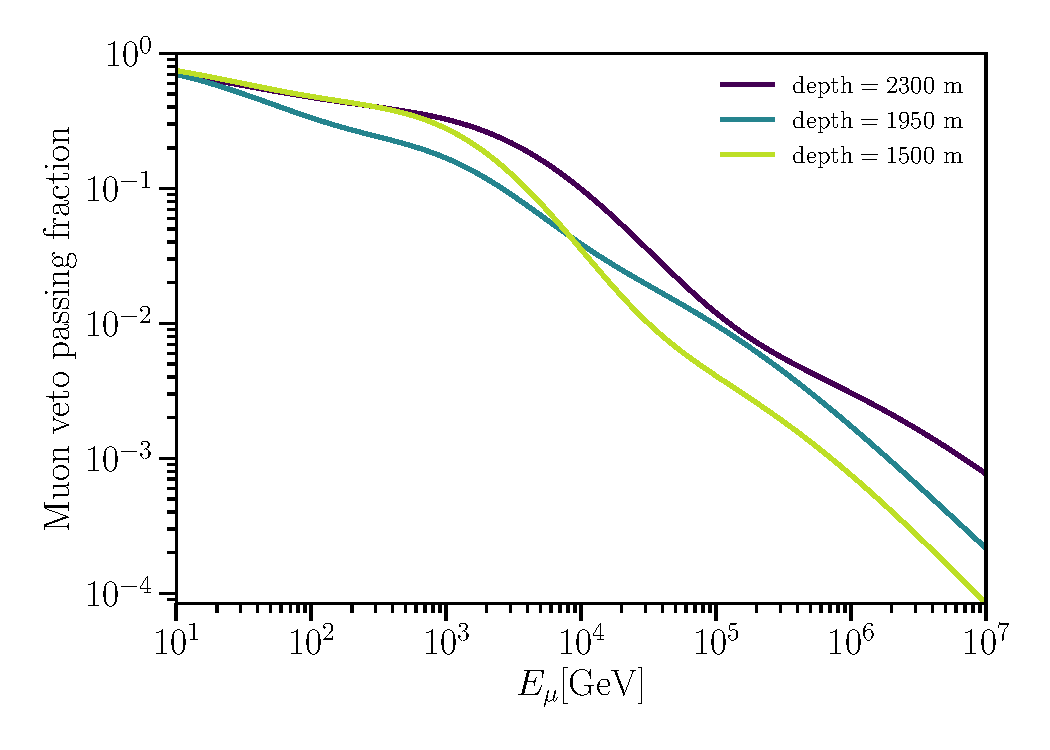
\includegraphics[width=\linewidth]{figures/hese_paper/plight}
	\internallinenumbers
	\caption{\textbf{\textit{Muon veto passing fraction.}} Each line shows the fraction of muons of a given energy, $E_\mu$, that pass without triggering the veto when entering the detector at a particular depth.
		Three depths are shown: 1500, 1950, and 2300 meters from the surface; with lines of darkening color as the depth increases.
		The veto efficiency increases with the muon energy.
		Differences at various depths are due to the changing ice properties and acceptance as a function of depth.}\label{fig:P_light}
\end{figure}

Using the passing fractions in \reffig{fig:P_light} as input and the \nuveto{} code provided in~\cite{Arguelles:2018awr} we calculate the atmospheric passing fraction for each component and flavor using the Hillas-Gaisser H3a~\cite{Gaisser:2013bla,Gaisser:2011cc,Hillas:2006ms} model for the incident cosmic-ray spectra and SIBYLL2.3c~\cite{Riehn:2017mfm} for the hadronic interactions in the air shower.
Using passing fractions derived from alternative cosmic-ray and hadronic interaction models has sub-leading effects in the determination of the astrophysical flux~\cite{Arguelles:2018awr}.
In this work, this was studied by repeating the analysis for different passing fractions that arise from a given combination of cosmic-ray spectrum and hadronic model for a variety of spectra and models that are available in the literature.
We found that the inclusion of these effects in addition to other discrete ice choices mentioned later increases the uncertainty of the astrophysical measurement by at most $\SI{20}\percent$ of existing errors.
In \reffigs{fig:passingfraction_conventional}{fig:passingfraction_prompt} we show the passing fractions for the conventional and prompt neutrino components.
In these figures the left, center, and right panels correspond to $\cos\theta_z$ values of 0.1, 0.3, and 0.9 respectively; the solid lines correspond to muon neutrinos and the dashed lines to electron neutrinos.
In the progression of the panels from left to right, one can see the passing fractions become smaller as one approaches vertical directions.
Vertical muons have the highest probability of reaching the detector, as the overburden they pass through is the smallest.
Though not shown in this figure, the conventional passing fractions differ from neutrinos to anti-neutrinos, see~\cite{Arguelles:2018awr} for details; in the analysis these differences are accounted for and figures for the anti-neutrino passing fractions can be found in~\cite{HESE:datarelease}.%TODO put these figures in the data release webpage
\reffigs{fig:conventional_distribution}{fig:prompt_distribution} show the distributions of conventional and prompt respectively after this correction is applied.
This reduction in atmospheric background is critical for measuring the astrophysical neutrino flux, as the observed down-going fluxes in IceCube would otherwise be comparable in magnitude and remain similar in their angular distribution.
This is best seen when comparing the atmospheric fluxes before and after the veto to the measured astrophysical flux as shown in \reffig{fig:neutrino_spectrum}.

% Plot of the passing fraction for different heights (one line per height) (one panel for each costh [3 values])
\begin{figure*}
	\centering
	\subfloat{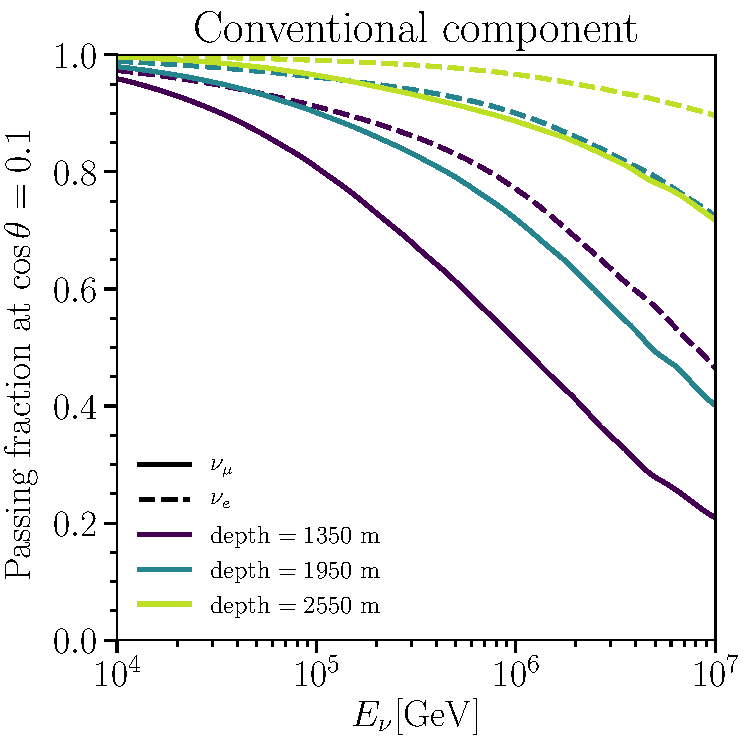
\includegraphics[width=0.3\linewidth]{figures/hese_paper/conv_0_1_passing_fraction}}
	\subfloat{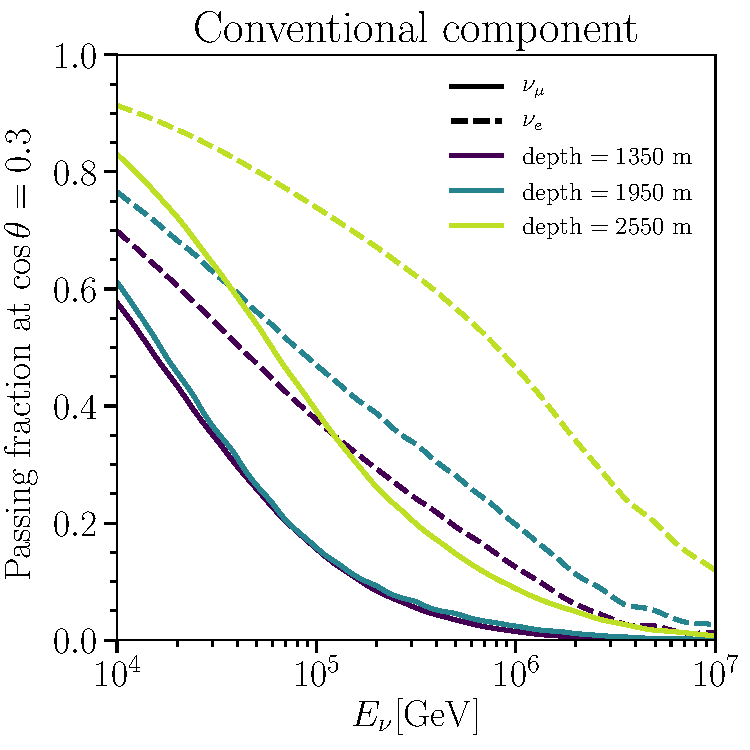
\includegraphics[width=0.3\linewidth]{figures/hese_paper/conv_0_3_passing_fraction}}
	\subfloat{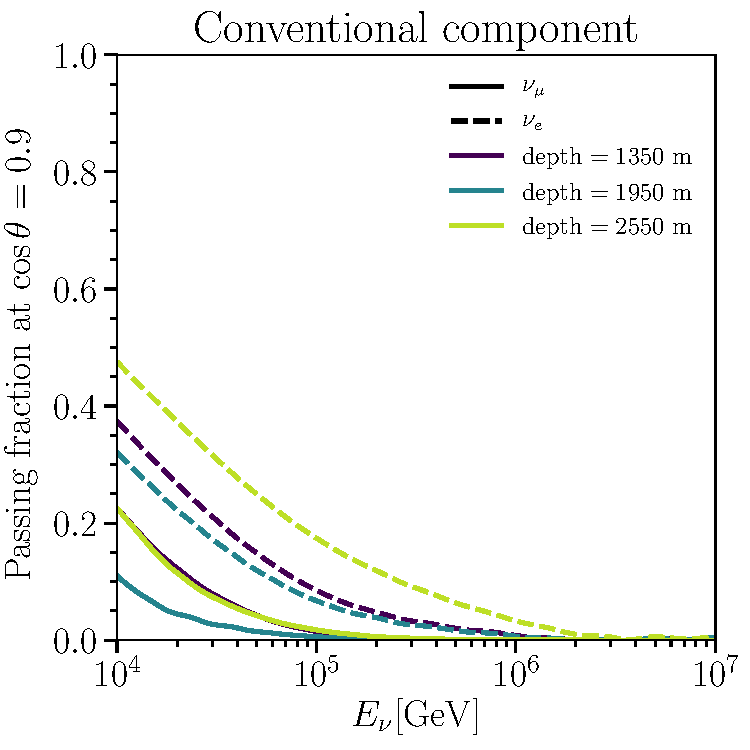
\includegraphics[width=0.3\linewidth]{figures/hese_paper/conv_0_9_passing_fraction}}
	\internallinenumbers
	\caption{\textbf{\textit{Conventional atmopheric component passing fraction.}}
		The atmospheric neutrino passing fraction is shown as a function of the neutrino energy, assuming the Hillas-Gaisser H3a~\cite{Gaisser:2013bla,Gaisser:2011cc,Hillas:2006ms} cosmic-ray model and SIBYLL 2.3c~\cite{Riehn:2017mfm} hadronic interaction model.
		Solid lines correspond to electron neutrinos and dashed lines to muon neutrinos.
		The different colors, from darkest to lightest, are for three different detector depths: 1350, 1950, and 2550 meters below the surface.
		The left, center, and right panel correspond to cosine of the zenith angles 0.1, 0.3, and 0.9 respectively (or zenith angles of $\SI{57}\degree$, $\SI{54.7}\degree$, and $\SI{35.6}\degree$).}\label{fig:passingfraction_conventional}
\end{figure*}

\begin{figure*}
	\centering
	\subfloat{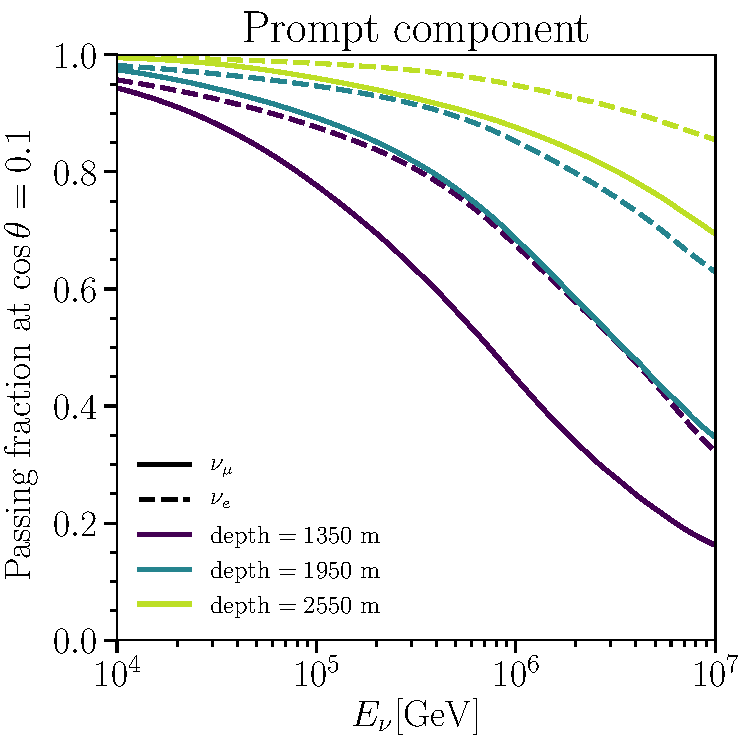
\includegraphics[width=0.3\linewidth]{figures/hese_paper/prompt_0_1_passing_fraction}}
	\subfloat{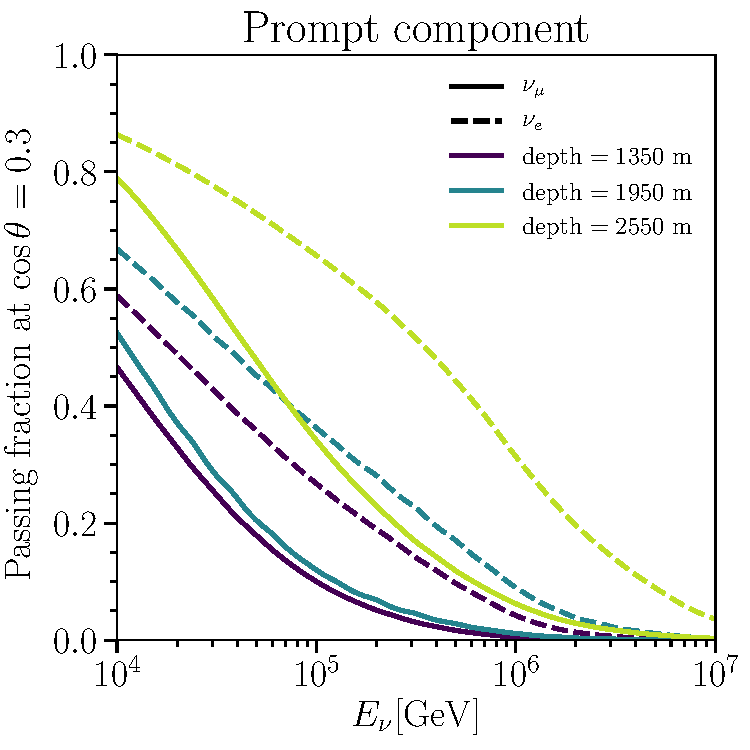
\includegraphics[width=0.3\linewidth]{figures/hese_paper/prompt_0_3_passing_fraction}}
	\subfloat{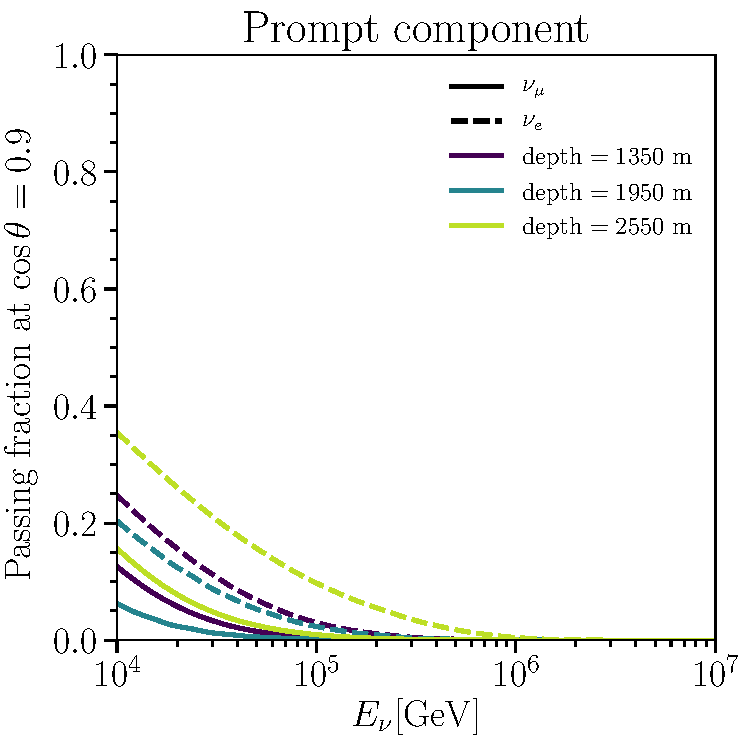
\includegraphics[width=0.3\linewidth]{figures/hese_paper/prompt_0_9_passing_fraction}}
	\internallinenumbers
	\caption{\textbf{\textit{Prompt atmospheric component passing fraction.}} Assumptions and line color coding are the same as in \reffig{fig:passingfraction_conventional}.}\label{fig:passingfraction_prompt}
\end{figure*}

\begin{figure}
	\centering
	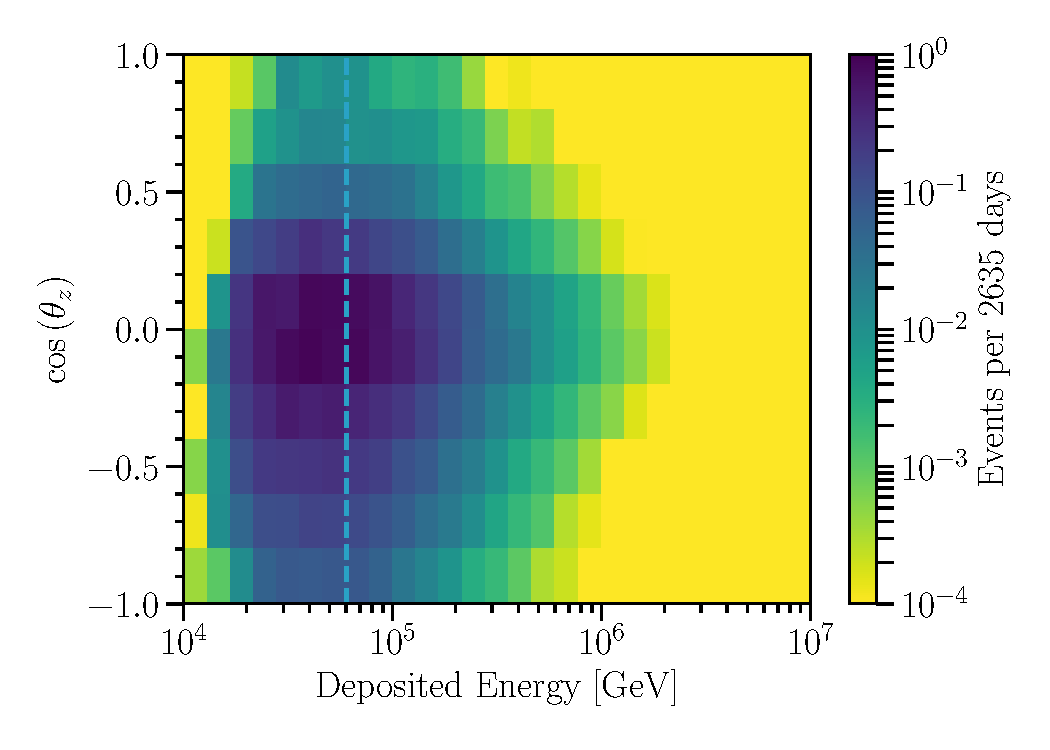
\includegraphics[width=\linewidth]{figures/hese_paper/diffuse_hist_all_conv}
	\internallinenumbers
	\caption{\textbf{\textit{Expected distribution of atmospheric neutrinos produced by pions and kaons in the sample.}} Distribution of neutrinos that pass the veto as a function of the deposited energy and the cosine of the zenith angle assuming nominal values for the nuisance parameters.
		The dashed line at $\SI{60}\TeV$ marks the low energy cut of the analysis.
		See \refsec{sec:systematics} for a discussion of the uncertainties associated with this component.}\label{fig:conventional_distribution}
\end{figure}

\begin{figure}
	\centering
	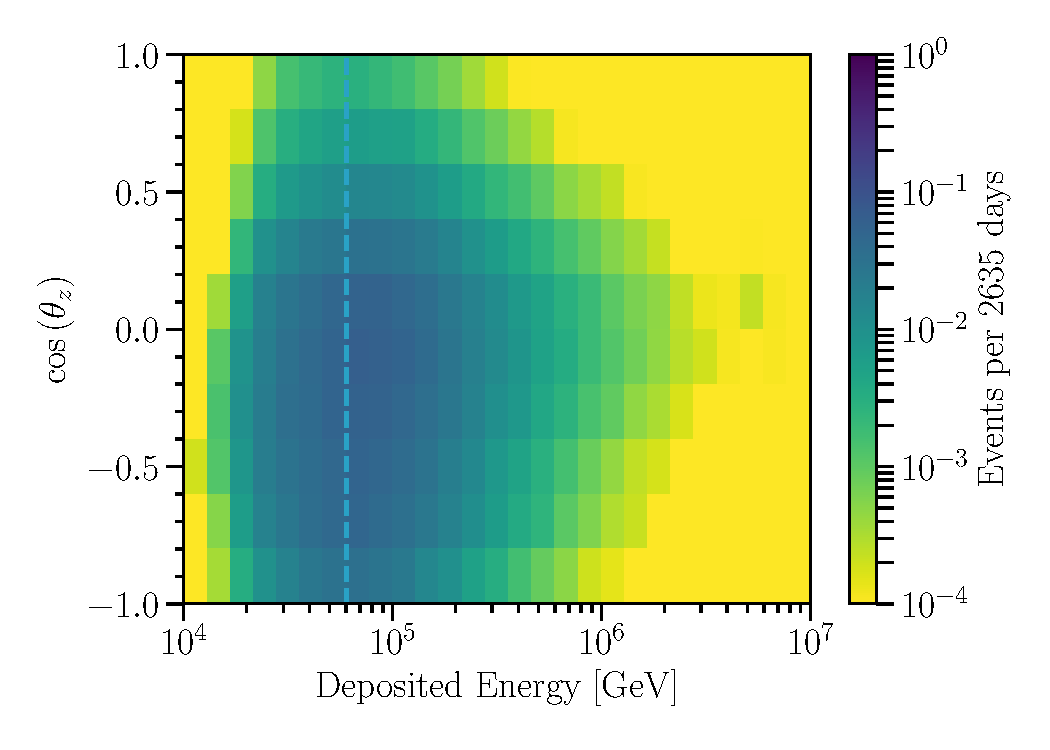
\includegraphics[width=\linewidth]{figures/hese_paper/diffuse_hist_all_prompt}
	\internallinenumbers
	\caption{\textbf{\textit{Expected distribution of atmospheric neutrinos produced by charm hadrons in the sample.}} Distribution of neutrinos that pass the veto as a function of the deposited energy and the cosine of the zenith angle assuming nominal nuisance parameters and production by charmed hadrons.
		The dashed line at $\SI{60}\TeV$ marks the low energy cut of the analysis.
		See \refsec{sec:systematics} for a discussion of the uncertainties associated with this component.}\label{fig:prompt_distribution}
\end{figure}

\begin{figure}
	\centering
	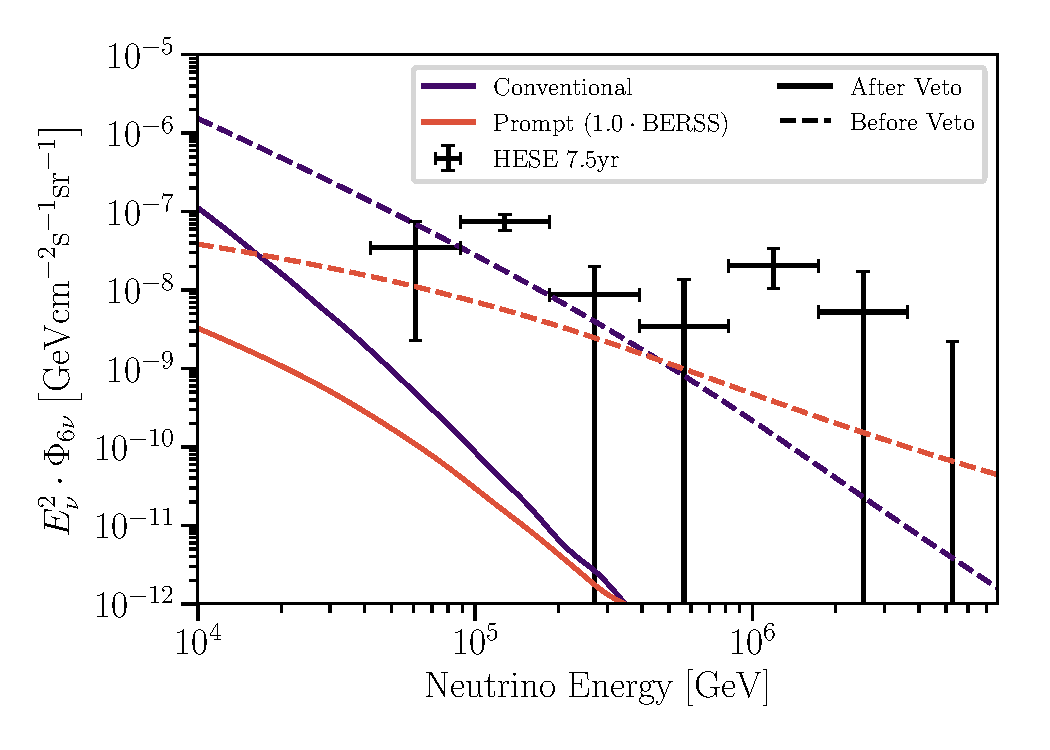
\includegraphics[width=\linewidth]{figures/hese_paper/neutrino_spectrum}
	\internallinenumbers
	\caption{\textbf{\textit{Astrophysical and atmospheric neutrino flux before and after the veto.}} The atmospheric neutrino fluxes considered in this analysis are shown as dashed lines.
		The solid lines show the product of the atmospheric flux with the passing fraction averaged over depth at a zenith angle of $\SI{0}\degree$.
		The frequentist segmented power-law fit of the astrophysical flux as described in \refsec{sec:generic_models} is shown in black.
		See \refsec{sec:systematics} for a discussion of the uncertainties associated with this component.}
	\label{fig:neutrino_spectrum}
\end{figure}

Finally there is also the possibility of single muons that trigger the event selection without a neutrino interaction in the detector and still pass the veto.
The flux of atmospheric muons from cosmic-ray air showers is modelled by a parameterization of muons from air showers simulated with the \CORSIKA~\cite{Heck:1998vt} package assuming the Hillas-Gaisser H4a~\cite{Gaisser:2013bla} cosmic-ray flux model and SIBYLL 2.1~\cite{Ahn:2009wx} hadronic model.
A dedicated single muon simulation, called \MUONGUN~\cite{jvsthesis}, is weighted to this flux. 
Due to the uncertainties in the muon yield of cosmic-ray air showers we use a data-based prior to constrain its normalization and only use the shape from simulation.
A second veto layer inside the original outer veto layer is introduced, and events that trigger the outer veto layer, but do not trigger this second inner veto layer, are tagged as muons that pass the inner veto.
The muon normalization from simulation is re-scaled from $N_\MUONGUN$ to $2.1\cdot N^\mu_\textmd{tagged}$ to match the number of tagged muons while accounting for the relative size of the fiducial volumes.
Thus, the baseline expected muon flux is given by
\begin{linenomath*}
	\begin{align}
	\frac{d^3\Phi}{d E_\mu d \theta_{z,\mu} d d_\mu} ={}& \Phi_\texttt{GaisserH4a}(E_\mu, \theta_{z,\mu},d_\mu)\\* & \cdot \frac{2.1 \cdot N^\mu_\textmd{tagged}}{N_\MUONGUN}
	\end{align}
	\label{eq:muon_scaling}
\end{linenomath*}
where $\Phi_\texttt{GaisserH4a}$ is the aforementioned parameterization; and $E_\mu$, $\theta_{z,\mu}$, and $d_\mu$ are the muon energy, zenith, and depth at injection respectively.
In \reftab{tbl:tag_muons} we list the number of tagged muons observed per year; in total 17 muons were observed.
The expected distribution of passing atmospheric muon events is shown in \reffig{fig:muons} as a function of the deposited energy and reconstructed cosine of the zenith angle.

\begin{figure}
	\centering
	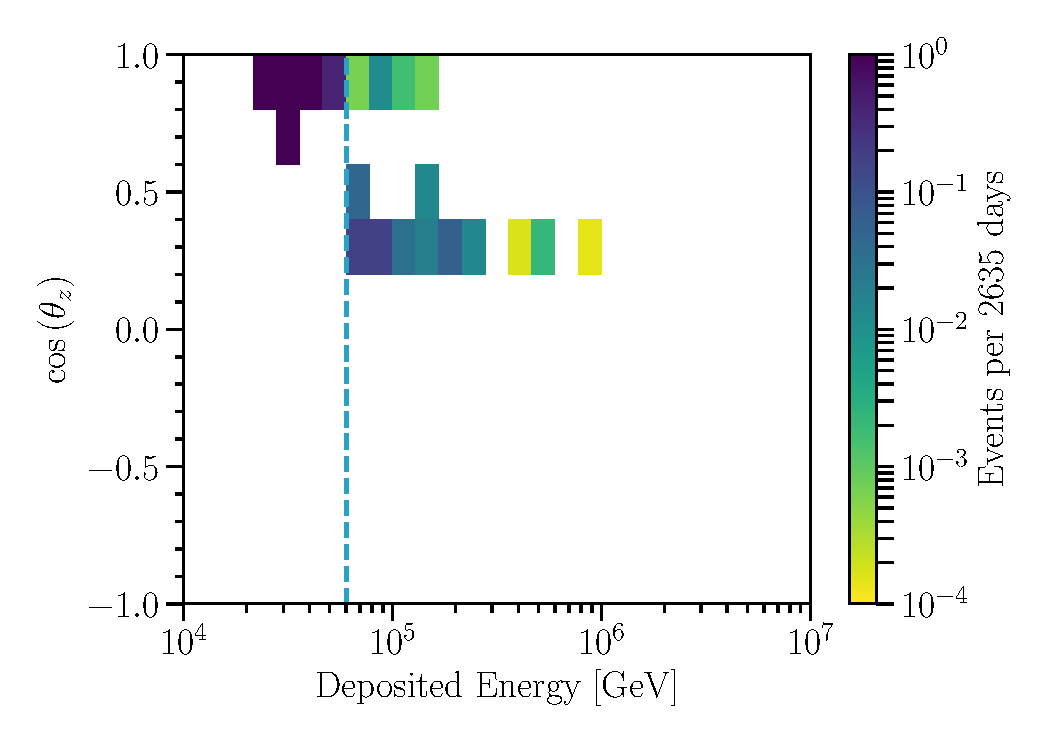
\includegraphics[width=\linewidth]{figures/hese_paper/diffuse_hist_all_muons}
	\internallinenumbers
	\caption{\textbf{\textit{Expected distribution of atmospheric muons in the sample.}} Distribution of muons that pass the veto as calculated with \MUONGUN~as a function of the deposited energy and the cosine of the zenith angle.
		The normalization is set to match the data driven sub-detector study.
		The dashed line at $\SI{60}\TeV$ marks the low energy cut of the analysis.}\label{fig:muons}
\end{figure}

\begin{table}
	\centering
	% year & number of tagged muons
	\begin{tabular}{l r}
		\toprule
		Year & $N^\mu_{tagged}$ \\
		\midrule
		2010 & 2 \\
		2011 & 1 \\
		2012 & 1 \\
		2013 & 1 \\
		2014 & 2 \\
		2015 & 6 \\
		2016 & 2 \\
		2017 & 2 \\
		\midrule
		Total & 17 \\
		\bottomrule
	\end{tabular}
	\internallinenumbers
	\caption{\textbf{\textit{Number of tagged muons per season.}}
		Table shows the number of tagged muons used to construct the muon normalization prior.
		The first year, 2010, used a partial IceCube configuration with 79 strings, the rest of the years of data taking were with the full configuration of 86 strings.}\label{tbl:tag_muons}
\end{table}

\section{Systematic uncertainties and statistical treatment\label{sec:systematics}}

\subsection{Detector systematic uncertainties\label{sec:detector_systematics}}

The main detector systematic uncertainties can be organized as arising from either incomplete knowledge of the ice properties or detector response.
The ice properties can in turn be separated into global ice effects -- such as anisotropy, scattering length, and absorption of photons in the bulk ice -- and local ice properties, {\it{}i.e.}\ effects of the re-frozen ice surrounding the DOMs previously melted during deployment~\cite{Karle:1994eua}.
In particular, additional air bubbles introduced in the drilling process and concentrated in the center of the hole during re-freezing increase the scattering of light, particularly in the vertical direction~\cite{Aartsen:2016nxy}.

We parameterize the uncertainties in the optical module light acceptance and local ice effects as three parameters called: DOM efficiency ($\domeff$), head-on efficiency ($\holeice$), and lateral efficiency ($\epsilon_\textmd{lateral}$).
The first parameter is an overall change in the efficiency of all of the DOMs in the detector, with respect to the individual baseline of each DOM.
The latter two parameters are part of a parameterization of the efficiency's angular dependence, which are discussed in greater detail in~\cite{Aartsen:2016nxy, Aartsen:2014yll, Aartsen:2017nmd}.
%
%The latter two parameters are part of a parameterization of the efficiency's angular dependence.
%In this parameterization the relative efficiency is
%\begin{linenomath*}
%        \begin{gather}
%        \begin{split}
%            A(\eta)={}&0.34\cdot(1+1.5\cdot\eta^3 / 2) + \\ & \epsilon_\textmd{lateral} \eta \cdot(\eta^2-1)^3 + \epsilon_\textmd{head-on} \cdot e^{10(\eta-1.2)},
%        \end{split}
%        \end{gather}
%    \label{eq:holeice}
%\end{linenomath*}
%where $\eta$ is the photon angle of incidence with respect to the photo-multiplier tube; see~\cite{Aartsen:2016nxy, Aartsen:2014yll, Aartsen:2017nmd} for a detailed discussion of this parameterization.
The $\holeice$ parameter modifies the photon efficiency in the vertical direction, while the $\epsilon_\textmd{lateral}$ parameter modifies the efficiency in the lateral direction.
Of these three parameters, only $\domeff$ and $\holeice$ have a significant effect on the observable distributions in this analysis, and so $\epsilon_\textmd{lateral}$ is fixed to a nominal value obtained from calibration data in the simulation used for this analysis.
To incorporate uncertainties that stem from these parameters into the analysis, we run dedicated simulation for values of relative $\domeff$.%: 0.81, 0.90, 0.95, 0.99, 1.08, and 1.17; where 0.99 corresponds to the nominal value.
Then, for each simulation, we construct two-dimensional histograms in the observed quantities for each neutrino flux -- {\it{}i.e.}\ conventional, prompt, and astrophysical -- and for each expected morphology -- {\it{}i.e.}\ cascade, track, and double cascade.
Comparing these observable distributions allows us to see the effect of $\domeff$.
We then smooth these histograms by constructing a spline using \PHOTOSPLINE~\cite{Whitehorn:2013nh,photospline}, resulting in a set of interpolating b-splines, one for each $\domeff$.
Finally, we linearly interpolate between the splines in the $\domeff$ dimension.
This systematic correction is applied multiplicatively to the expectation of the sample.
The result of applying this correction is shown in the appendix \reffig{fig:domeff}.

A similar procedure is performed to include the effect of changing the head-on efficiency.
Again, we run dedicated simulation for several values of $\holeice$ to compute the systematic correction.%, in this case: -3, -1, 0, and 1; where 0 corresponds to the nominal value~\cite{Aartsen:2013rt}.
This correction is also applied multiplicatively to the expectation resulting in the distributions in appendix \reffig{fig:holeice}, where we vary this parameter in the one sigma range.

The global properties of the ice are taken into account in different ways for different effects.
The scattering and absorption of photons in the ice is azimuthally anisotropic because of the ice flow~\cite{Aartsen:2013rt}.
For the dedicated tau search performed in this analysis, which relies on the double cascade morphology, the reconstructed length between the energy depositions is modified as a function of the orientation with respect to the anisotropy axis and the strength of the anisotropy.
The anisotropy axis is well constrained by calibration measurements, however the strength of this effect is more uncertain.
%TODO add appropriate reference for tau paper
We incorporate the uncertainties of this effect by parameterizing the bias in the length reconstruction with an analytic function; see~\cite{HESETAU} for details.
The effect of this bias on the distribution of event observables is then parameterized with splines in the same way as the previously mentioned ice and detector systematics.
The result of applying this change in anisotropy to this sample is shown in appendix \reffig{fig:anisotropy}.
Other observables are not strongly affected by this systematic uncertainty, so the effect is neglected.

The bulk ice scattering and absorption uncertainty is sub-leading and the impact is evaluated by repeating the analysis with three different ice variants.
The three ice variants used are: a $\SI{10}\percent$ increase in overall light scattering, a $\SI{10}\percent$ increase in overall light absorption, and a simultaneous $\SI{7.5}\percent$ reduction of both absorption and scattering.
We found that the inclusion of these effects in combination with the effects of bulk ice scattering, bulk ice absorption, and the previously mentioned discrete atmospheric flux choices increases the uncertainty of the astrophysical measurement by at most $\SI{20}\percent$ of existing errors.

\subsection{Statistical treatment\label{sec:statistics}}

We group the model parameters described in this section into two categories: parameters of interest ($\vec\theta$) and nuisance parameters ($\vec\eta$).
The former depend on the analysis and the latter include parameters that modify the systematic effects discussed in \refsec{sec:detector_systematics}, as well as physics parameters not being examined.
The physics model parameters of interest, which are discussed in greater detail in \refsec{sec:diffuse}, often refer solely to the astrophysical model parameters.
In the case of a single power-law astrophysical flux hypothesis these are the astrophysical neutrino flux normalization ($\Phi_{\textrm astro}$)  and the spectral index of the power-law flux ($\gamma_{\textrm astro}$).
Different parameters of interest are given for other generic astrophysical models in \refsec{sec:generic_models} and source-specific models in \refsec{sec:specific_models}.
In the case of searches for new physics, more terms are incorporated into the model parameters; {\it{}e.g.} for the dark matter decay search: the dark matter mass and its lifetime.
In all cases we will use the same systematic treatment of the relevant uncertainties described in \refsec{sec:detector_systematics}.

In the analyses presented in this paper, as well as associated results shown in~\cite{HESEFLV,HESEDM, HESEXS}, we present our results using both the frequentist and Bayesian statistical methodologies.
These two methodologies provide distinct information, the frequentist techniques make statements about the plausibility of the data given a model, while the Bayesian techniques make statements about the model.
In the frequentist framework, the parameters that most likely explain the data are obtained and reported.
We also report intervals in parameter space constructed such that they contain the true value of the parameter some fraction of the time for repeated experiments.
These constructions free us from dependence on priors, but do not inform us of the model parameters; see~\cite{Biller:2014eya} for an extended discussion on caveats of confidence intervals.
On the other hand, the Bayesian framework makes statements about the model by invoking Bayes theorem, at the cost of a dependence on prior choice.
In this framework, we report the most probable model parameters given the observed data, and the preferred regions of parameter space.
%Nevertheless, frequentist techniques can provide calibrated expectations, namely, if the $p$-value for the observed data is found to be too small, this suggest that something odd is going on with respect to the reference model.
Thus, frequentist and Bayesian methods can be both be applied and provide complementary information about the model and the data; see~\cite{Diaz:2019fwt} for a review and comparison of these methods in the context of neutrino experiments.
For both of these approaches we will make use of the likelihood function, which reflects the plausibility of model parameters given observed data and is defined as $\like(\vec\theta, \vec\eta) = p(\textrm{data}|\vec\theta, \vec\eta)$.
Where $p(\textrm{data}|\vec\theta, \vec\eta)$ is the probability of the data given the model parameters.
We also include external knowledge of the model parameters as the term $\Pi(\vec\theta, \vec\eta)$, which is the constraint (prior) on the parameters in the frequentist (Bayesian) interpretation.
Details of $\Pi$ are given in \reftab{tbl:priors}.

For our frequentist results we present the best-fit parameters and their errors using the profile likelihood technique to construct the model parameter test statistic
\begin{linenomath*}
	\begin{equation}
	\tilde{\like}^\texttt{profile}(\vec\theta) = \max_{\vec\eta} \like(\vec\theta,\vec\eta)\cdot\Pi(\vec\theta, \vec\eta),
	\label{eq:likelihood_freq}
	\end{equation}
\end{linenomath*}
where we minimize the negative log of the function in place of maximizing the function.
%This minimization is performed over continuous nuisance parameters using the L-BFGS-B algorithm~\cite{doi:10.1137/0916069}.
Maximizing $\tilde{\like}^\texttt{profile}$ over all parameters defines the best-fit point $\hat{\vec\theta}$.
Our frequentist results are then presented assuming Wilks' theorem~\cite{wilks1938}, see~\cite{Algeri:2019arh} for a recent summary of the conditions under which this theorem holds, and with the appropriate degrees of freedom, where the test-statistic ($\TS$) is defined as
\begin{linenomath*}
	\begin{equation}
	\TS = -2\log{\left(\frac{\tilde{\like}^\texttt{profile}(\vec\theta)}{\tilde{\like}^\texttt{profile}(\hat{\vec\theta})}\right)}.
	\end{equation}
\end{linenomath*}

The product of $\like(\vec\theta, \vec\eta)$ and $\Pi(\vec\theta, \vec\eta)$ can be normalized to form a probability distribution of the model parameters known as the posterior distribution.
The posterior distribution encodes the information about the model parameters after being updated by the observed data~\cite{RevModPhys.83.943}, and is used to present many of the Bayesian results of this work.
This probabilistic interpretation allows one to determine the regions of parameter space that have the largest probability of containing the parameter~\cite{laplace1820theorie}.
Integrating the posterior over the nuisance parameters and normalizing, we obtain the marginal posterior
\begin{linenomath*}
	\begin{equation}
	\mathcal{P}(\vec\theta) = \frac{\int d\vec\eta~\like(\vec\theta,\vec\eta) \Pi(\vec\theta,\vec\eta)}{\int d\vec\theta d\vec\eta~\like(\vec\theta,\vec\eta) \Pi(\vec\theta,\vec\eta)}.
	\label{eq:likelihood_bayes}
	\end{equation}
\end{linenomath*}
Practically, this is achieved using an affine-invariant Markov Chain Monte Carlo (MCMC) called \texttt{EMCEE}~\cite{ForemanMackey:2012ig} to sample the posterior distribution, and examining the distribution of samples in $\vec\theta$~\cite{RevModPhys.83.943}.
%A Markov Chain is a series of random variables, namely $\{\vec\psi_i\}=\{(\vec\theta_i,\vec\eta_i)\}$, such that the probability distribution of any variable in the chain only depends on the value of the previous iteration.
%For appropriate transition probabilities, which dictate the probability of going from $\vec\psi_i$ to $\vec\psi_{i+1}$, it can be shown that the distribution of these random variables converges to the desired posterior distribution; for a complete discussion see~\cite{RevModPhys.83.943}.

In the case that our model parameter posterior is confined to a compact region we report the highest-posterior-density (HPD) credible region of that parameter, and its maximum {\it{}a posteriori} (MAP) estimation.
However, there are some cases where credible regions are ill-defined, or a natural choice of prior is not immediately clear.
In these scenarios we report our results using the Bayes factor as a function of the model parameter~\cite{Trotta:2017wnx}, {\it i.e.}\ the ratio of the evidence between the alternative physics model and the null hypothesis,
\begin{linenomath*}
	\begin{equation}
	\mathcal{B}_{1 0} = \frac{\int d\vec\theta' d\vec\eta'~\mathcal{L}_\texttt{\tiny{1}}(\vec\theta',\vec\eta')\cdot\Pi_\texttt{\tiny{1}}(\vec\theta',\vec\eta')}{\int d\vec\theta d\vec\eta~\mathcal{L}_\texttt{\tiny{0}}(\vec\theta, \vec\eta)\cdot\Pi_\texttt{\tiny{0}}(\vec\theta,\vec\eta)},
	\label{eq:bayes_factor}
	\end{equation}
\end{linenomath*}
where the evidence is the integral of the un-normalized posterior over all model parameters.
Given a Bayes factor it is customary to assign a qualitative description.
For this we use Jeffreys' scale~\cite{jeffreys1998theory}, which we reproduce in \reftab{tbl:jeffrey}.
In this case, to compute the model evidence we use the \texttt{MultiNest} package~\cite{Feroz:2013hea}.

\begin{table}
	\begin{center}
		\begin{tabular}{c|c}
			\hline
			Bayes factor ($\mathcal{B}$) range & Inference convention \\
			\hline
			$\mathcal{B} <1$ & $\Theta_0$ favored \\
			$1<\mathcal{B}<10^{1/2}$ & $\Theta_1$ barely favored\\
			$10^{1/2}<\mathcal{B}<10^{1}$ & $\Theta_1$ substantially favored\\
			$10^{1}<\mathcal{B}<10^{3/2}$ & $\Theta_1$ strongly favored\\
			$10^{3/2}<\mathcal{B}<10^{2}$ & $\Theta_1$ very strongly favored\\
			$\mathcal{B} > 10^{2} $ & $\Theta_1$ decisively favored\\
			\hline
		\end{tabular}
	\end{center}
	\internallinenumbers
	\caption{\textit{\textbf{Bayes factors and Jeffreys' scale inference convention.}}
		The left colum shows the range of the Bayes factor, $\mathcal{B}$, between the null hypothesis, $\Theta_0$, and an alternative hypothesis, $\Theta_1$.
		The right column shows the inference convention according to Jeffreys' scale~\cite{jeffreys1998theory}.}
	\label{tbl:jeffrey}
\end{table}

In order to evaluate the likelihood function, it is necessary to compute the expected number of events in each observable bin given the model parameters.
This expectation is obtained through Monte Carlo simulation of the detector.
The IceCube Monte Carlo is computationally expensive at high energies, so much so that it is prohibitive to produce MC such that the statistical fluctuations of the MC are much smaller than the data fluctuations for the atmospheric muon background.
In order to avoid making incorrect statements due to the large MC statistical uncertainty in some bins, the analyses described in \refsec{sec:diffuse} use a modified Poisson likelihood function, $\likeSAY$, that accounts for MC statistical uncertainty~\cite{Arguelles:2019izp}.
This treatment produces similar results to other treatments available in the literature~\cite{Chirkin:2013lya,Glusenkamp:2017rlp,Glusenkamp:2019uir}, but provides improved coverage properties, is numerically more stable, and is computationally more efficient~\cite{Arguelles:2019izp}.
The likelihood for this analysis is given by
\begin{linenomath}
	\begin{align}
	\begin{split}
	\like(\vec\theta, \vec\eta) ={}& \left[\prod_j^{n} \likeSAY(\mu_j(\vec\theta,\vec\eta), \sigma_j(\vec\theta,\vec\eta); d_j) \right]\label{eq:likelihood}
	\end{split}
	\end{align}
\end{linenomath}
and the priors/constraints by
\begin{linenomath}
	\begin{align}
	\begin{split}
	\Pi(\vec\theta, \vec\eta)={}& \left[\prod_r \Pi_r(\theta_r)\right] \cdot \left[\prod_s \Pi_s(\eta_s) \right],\label{eq:priors}
	\end{split}
	\end{align}
\end{linenomath}
where $j$ refers to the bin number, $r$ indexes the parameters of interest, and $s$ indexes the nuisance parameters.
The variables $\theta_r$ and $\eta_r$ denote the parameters of interest and nuisance parameters respectively.
The arguments of the likelihood $\mu_j$ and $\sigma_j$ are the expected number of events and MC statistical uncertainty of that quantity respectively, while $d_j$ is the number of observed data events in that bin.
The parameters $\vec\theta$ and $\vec\eta$ have priors/constraints which are represented in Eq.~\eqref{eq:priors} by $\Pi_r(\theta_r)$ and $\Pi_s(\eta_s)$ respectively and are enumerated in \reftab{tbl:priors}.
Improper uniform priors are used for parameters that otherwise have unspecified priors.
There are $630$ bins in observable quantities used in the analysis.
Events are first separated by their inferred morphology.
Track and cascade events are then binned separately with the same strategy; twenty one divisions are made in deposited energy starting at $\SI{60}\TeV$, spaced equally in the log of the energy such that each pair of bin edges satisfies $\Delta\log_{10} ( E_\textmd{bin edge} / \SI{1}\GeV)=0.111$ (except for the highest energy bin which is truncated at $\SI{10}\PeV$), and ten divisions in reconstructed zenith equally spaced in $\cos\theta_z$ for a total of 210 bins for tracks and 210 bins for cascades.
For double cascades we neglect the zenith information, binning only in reconstructed energy and length; twenty one divisions are made in energy in the same way as for tracks and cascades, and ten divisions are made in the reconstructed length, starting at $\SI{10}\meter$ and spaced equally in the log of the length such that each pair of bin edges satisfies $\Delta\log_{10} (l_\textmd{bin edge} / \SI{1}\meter)=0.1$ for a total of 210 bins for double cascades.
The bin widths are chosen to be comparable to the detector resolution.

\section{Characterization of the astrophysical neutrino flux\label{sec:diffuse}}

\noindent
\textit{We find that the astrophysical component observed in HESE is well described by a single power law with a spectral index of $\SPLFreqWilksIndexSummary$.
	Other generic parameterizations of the astrophysical flux are also considered, but none represent a significant improvement over the single power-law hypothesis.
	In these generic models the preferred regions of parameter-space are degenerate with the single power-law model.
	We also introduce a generic parameterization of the flux comprised of a set of flux segments, and report the segment normalizations and uncertainties.
	In this sample we find no evidence of an atmospheric neutrino flux from the decay of charmed hadrons and find that prompt normalizations greater than $\sim 13$ times the baseline prompt model are strongly disfavored; the obtained limit is weaker than existing constraints obtained from other samples.
	Finally, we study proposed source models, testing if they are preferred compared to a baseline scenario.
	We find that no source model scenario is strongly favored with respect to the baseline single power-law model of the astrophysical neutrino flux.
}
\newline

As the sources of the astrophysical neutrino flux are largely unknown~\cite{Albert:2017ohr,Aartsen:2018ywr,Aartsen:2019epb}, we take a two pronged approach to characterize the astrophysical spectrum.
In \refsec{sec:generic_models} we consider generic forms for the spectrum, which could arise from a large number of physical scenarios.
\refsec{sec:prompt} explores the atmospheric flux of neutrinos from charmed hadrons.
In \refsec{sec:specific_models} we test a small sample of spectra from the literature.
We provide the data, Monte Carlo, and tools necessary for these tests in the data release outlined in \refappsec{sec:release} and encourage readers to perform their own tests of model compatibility~\cite{HESE:datarelease}.

In addition to the spectral models chosen, three key assumptions are made about the astrophysical neutrino flux in this section: the flux incident on Earth is isotropic, it is the same between neutrinos and anti-neutrinos, and the same for each neutrino flavor.
An isotropic flux is expected in models where the dominant contribution is from distant sources.
We focus on the isotropic flux hypothesis as it agrees well with available neutrino data.%, and will revisit this assumption as sources are identified.
The IceCube detector is insensitive to the differences between neutrino and anti-neutrino interactions on an event by event basis for most energies, and so differences between the neutrino and anti-neutrino flux content do not modify the expectation of detected events in this analysis for most energies.
The one region where this does not hold is for electron anti-neutrinos near $\SI{6.3}\PeV$ where the resonant interaction of electron anti-neutrinos with atomic electrons called the Glashow Resonance (GR)~\cite{Glashow:1960zz,Loewy:2014zva} can occur.
This enhances the expectation of detected down-going events near the resonance energy, and reduces the expectation for vertically up-going events~\cite{Barger:2014iua}.
%TODO fix these references
However, because the spectrum is steeply falling, as observed in previous analyses~\cite{Aartsen:2016xlq,Aartsen:2014gkd}, the expected number of GR events is small in comparison to the rest of the sample.

As described in \refsec{sec:backgrounds}, backgrounds from cosmic-ray showers produced in the Earth's atmosphere are a non-negligible contribution to the events observed in the sample.
The background model used throughout this section includes atmospheric neutrinos from pions, kaons, and charmed hadrons, as well as atmospheric muons.
\reftab{tbl:priors} describes the parameters of the fit for the single power-law model and the priors (or constraints) associated with them.
In addition to the astrophysical model and backgrounds with their respective nuisance parameters, detector systematics are also included in the model.
Only the parameters of the astrophysical neutrino flux differ between the models described in this section, the background models and detector systematics remain the same.

\subsection{Generic models\label{sec:generic_models}}

Many well-motivated models of the astrophysical neutrino flux come in the form of power laws.
This commonality stems from the possibility that astrophysical neutrinos and cosmic rays may share a common origin, and that we observe cosmic rays at Earth with a power-law spectrum.
To examine the possibility of a power-law-like flux we study a few generic scenarios for the astrophysical flux in the following sections.
The first scenario, called the ``single power law'' (SPL), is an unbroken power law across all energies with a freely varied normalization and spectral index.
This is the simplest model as it only has two free parameters for the astrophysical spectrum: spectral index and normalization.
It is also motivated by Fermi-acceleration, which predicts a power-law energy spectrum.
The second scenario, called the ``double power law'' (DPL), is the sum of two unbroken power-law spectra, both with freely varying normalizations and spectral indices.
This potentially describes scenarios in which there are two populations of sources, two production mechanisms for high-energy astrophysical neutrinos that produce different power-law fluxes, or where neutrinos and anti-neutrinos have different spectra~\cite{Nunokawa:2016pop,Shoemaker:2015qul}.
A variety of source production models predict a high-energy cutoff in the neutrino spectrum, whether from limitations of the source energetics, a drop in pion production efficiency, energy losses of secondary pions and muons, or other mechanisms.
To accommodate this possibility in a functionally simple way, we define a model with a single power-law astrophysical flux that has an exponential suppression at high energies.
This third scenario, called the ``exponential cutoff,'' has an additional parameter describing the energy scale of the cutoff.
The fourth scenario, called the ``log parabola'' (LP), is a simple extension to the power law.
While a power law can be represented as a line in log-log space, the log-parabola adds curvature in log-log space.
This model is often used to describe gamma ray spectra across many orders of magnitude of gamma ray energy, which could otherwise be described as power laws in smaller energy ranges~\cite{TheFermi-LAT:2017pvy}.

\subsubsection{Single power-law flux\label{sec:spl}}

\noindent
\textit{%Here we describe the single power-law model analysis.
	Our main finding is that a single power law, with a spectral index of $\SPLFreqWilksIndexSummary$, is a good description of the observed data.
	This result has been robust under the improved systematic treatment of this analysis, and is softer than previously reported results predominantly due to the large excess of lower energy events with respect to the atmospheric background.
	The introduction of an additional prompt neutrino flux is only weakly correlated with the measured astrophysical spectral index and it primarily affects uncertainty of the astrophysical normalization measurement.
}
\newline

\begin{figure*}
	\centering
	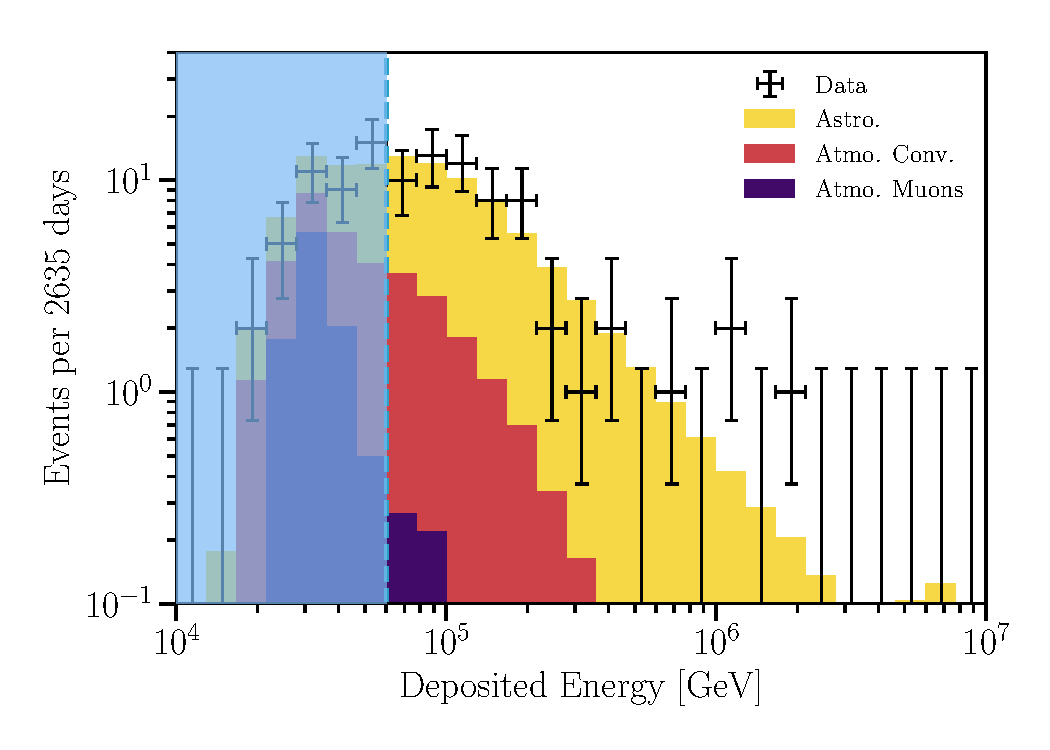
\includegraphics[width=0.45\linewidth]{figures/hese_paper/diffuse_energy_projection_all}
	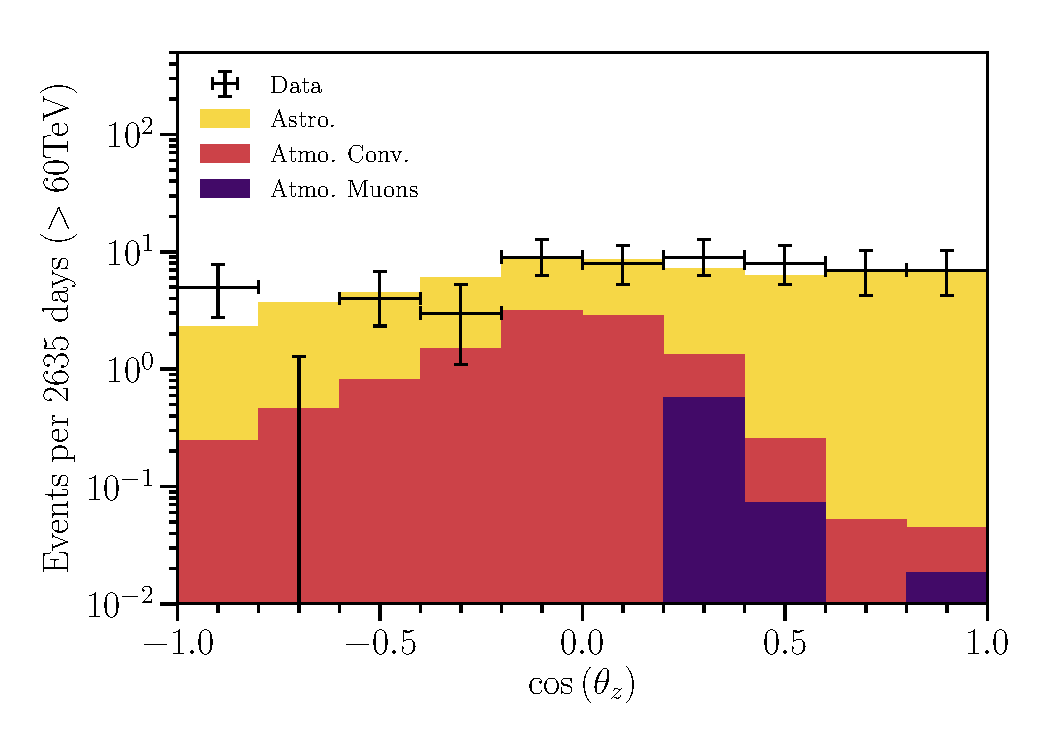
\includegraphics[width=0.45\linewidth]{figures/hese_paper/diffuse_zenith_projection_all}
	\internallinenumbers
	\caption{\textbf{\textit{Deposited energy and reconstructed $\cos\theta_z$ distributions.}}
		In these panels the data is shown as crosses and the best-fit expectation as a stacked histogram with each color specifying a given flux component: astrophysical neutrinos (golden), conventional atmospheric neutrinos (red), and penetrating atmospheric muons (purple).
		Left: distributions of events and expected event count assuming best-fit parameters as a function of the deposited energy; events below $\SI{60}\TeV$ (light blue vertical line) are ignored in the fit.
		Right: distribution of events with energy greater than $\SI{60}\TeV$ in the cosine of their reconstructed zenith angle.
		Up-going events are on the left side of this panel and down-going events on the right.
		The expected number of events are split by components and displayed as a stacked histogram.
		The normalization of the prompt atmospheric neutrino component fits to zero and so is not shown in the stacked histogram.
		The distribution of data events appears to be largely flat as a function of cosine zenith with some systematic deficit in the up-going region.
		The deficit in the up-going region is expected as a result of the Earth's absorption of the neutrino flux, and appears to be compatible with the Monte Carlo expectation.}\label{fig:energy-zenith}
\end{figure*}

For the single power-law-flux scenario, we assume that there is an isotropic flux of astrophysical neutrinos incident on the Earth with a total differential all-flavor neutrino-plus-anti-neutrino spectrum given by
\begin{linenomath*}
	\begin{gather}
	\begin{split}
	\frac{d\Phi_{6\nu}}{dE} =&{}~\Phi_\texttt{astro}{\left(\frac{E_\nu}{\SI{100}\TeV}\right)}^{-\gamma_\texttt{astro}} \\
	& \cdot 10^{-18}~[\textmd{GeV}^{-1}\textmd{cm}^{-2}\textmd{s}^{-1}\textmd{sr}^{-1}].
	\end{split}
	\label{eq:spl_flux}
	\end{gather}
\end{linenomath*}
Where $\Phi_{6\nu}$ is the flux of the six neutrino species combined, $\astronorm$ is the normalization, and $\astrodeltagamma$ is the common spectral index.
These two parameters are incorporated as arguments of the likelihood according to \refsec{sec:statistics}.
To better understand the relationship between the data and the neutrino flux contributions, we first look at projections in the two observables most different between neutrino fluxes (zenith, and energy) and compare data to the expectation from Monte Carlo assuming the nuisance parameters from the best-fit ($\hat{\vec\theta},\hat{\vec\eta})=\argmax_{\vec\theta, \vec\eta} \like(\vec\theta,\vec\eta)\cdot\Pi(\vec\theta,\vec\eta)$).
The right panel of \reffig{fig:energy-zenith} shows the data and expected number of events in bins of the cosine of the reconstructed zenith angle.
In the down going region the data seem to be well described with the addition of an isotropic astrophysical neutrino flux.
Atmospheric components alone are not capable of describing the data well, because the atmospheric components are suppressed in the down-going region; see \refsec{sec:prompt} for details.
In fact the atmospheric only hypothesis is rejected with respect to the addition of an astrophysical component at a level greater than $5\sigma$ with this sample.
The left panel of \reffig{fig:energy-zenith} shows the data and expected number of events in bins of reconstructed deposited energy.
The region below $\SI{60}\TeV$ is not included in the analysis because of larger background uncertainties, however we present the data to MC comparison in this region to demonstrate the level of agreement below the cut.
From the stacked histogram it is clear that the sample is dominated by the astrophysical component above $\SI{60}\TeV$.

% SPl parameter information
\begin{figure}
	\centering
	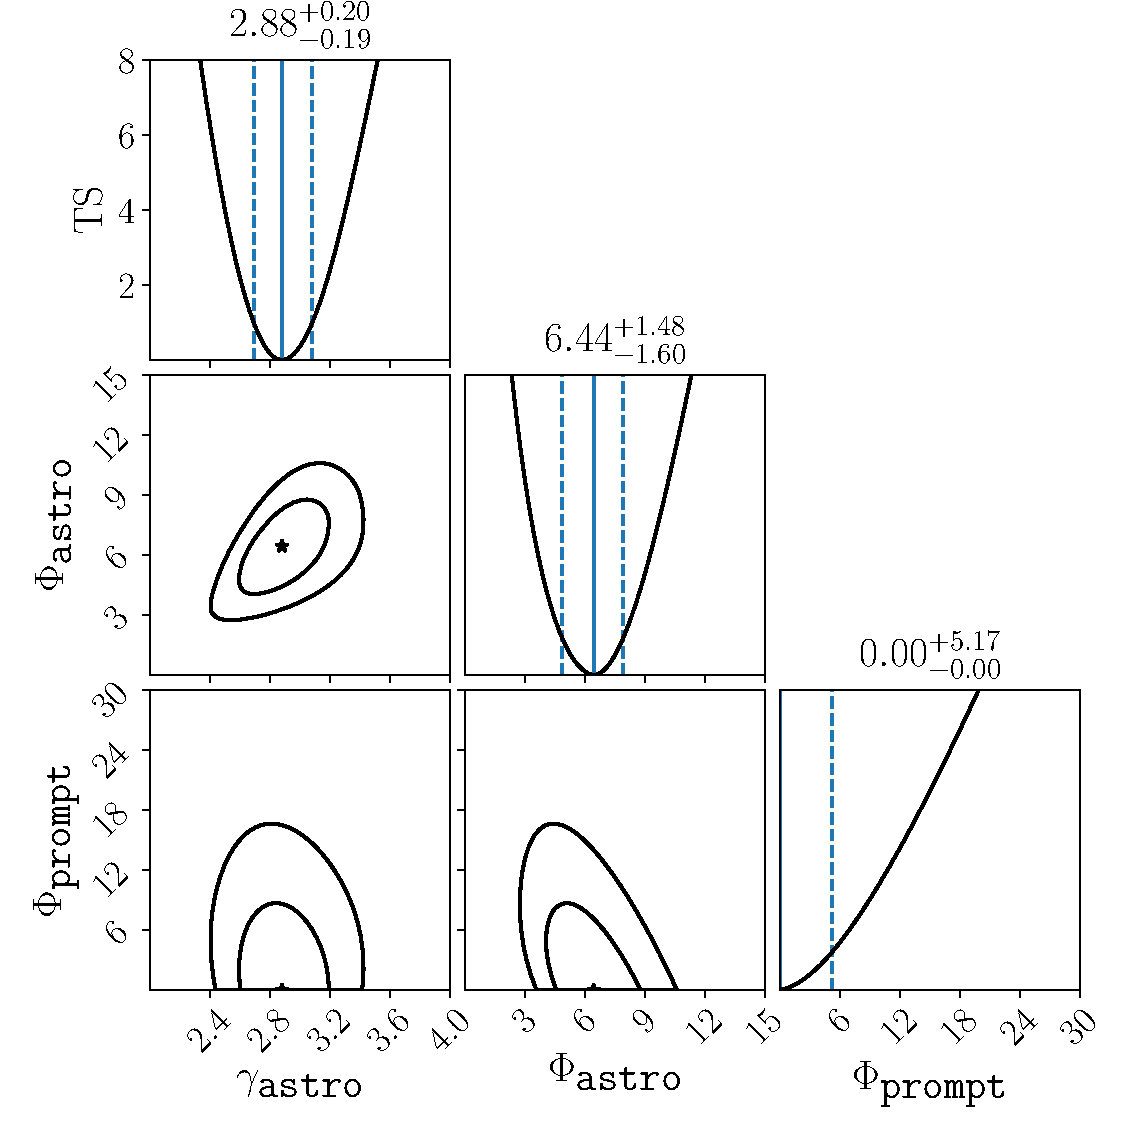
\includegraphics[width=\linewidth]{figures/hese_paper/freq_corner}
	\internallinenumbers
	\caption{\textbf{\textit{Single power-law profile likelihood.}}
		Diagonal panels show the $\TS$, as a function of different model parameters, and the one sigma intervals assuming Wilks' theorem.
		Other panels show the best-fit point and two-dimensional contours.
		Solid (dashed) contours represent the $\SigmaOne$ ($\SigmaTwo$) confidence regions assuming Wilks' theorem.}\label{fig:SPL_profile}
\end{figure}

% SPL parameter information
\begin{figure}
	\centering
	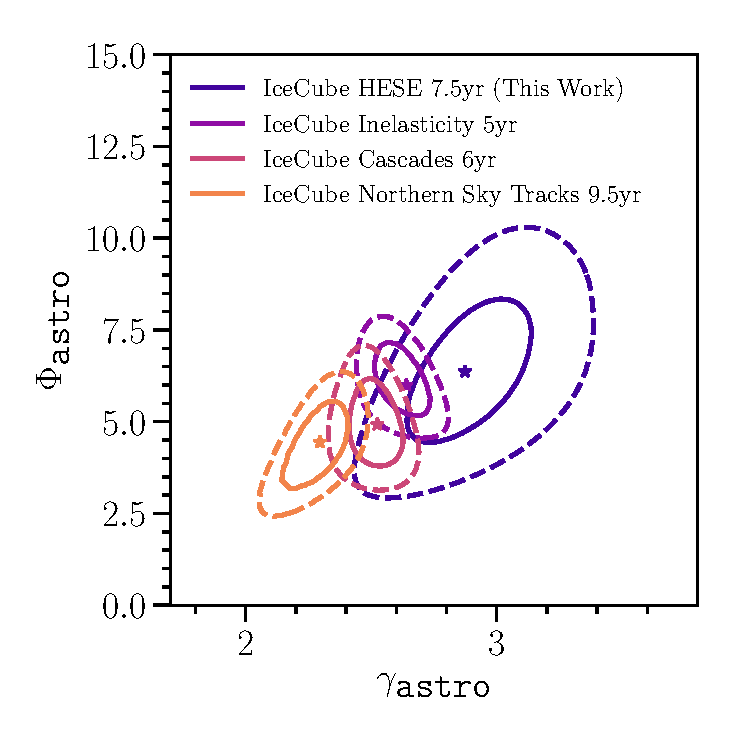
\includegraphics[width=\linewidth]{figures/hese_paper/spl_freq_scan}
	\internallinenumbers
	\caption{\textbf{\textit{Comparison of single power-law parameters from different analyses.}} Assuming an unbroken single power-law model for the astrophysical neutrino flux, results from different IceCube samples are shown.
		The horizontal axis is the spectral index of the model and the vertical axis is six-neutrino flux normalization at $\SI{100}\TeV$ given in units of $10^{-18}~[\textmd{GeV}^{-1} \textmd{sr}^{-1} \textmd{s}^{-1} \textmd{cm}^{-2}]$.
		The stars denote the different best-fit points, solid contours show the $\SigmaOne$ confidence region using the asymptotic approximation given by Wilks' theorem, and dashed contours show the $\SigmaTwo$ confidence regions.
		Blue represents results from this work, while the purple shows results from IceCube's 5yr inelasticity measurement~\cite{Aartsen:2018vez}, salmon shows results from IceCube’s 6yr cascade sample~\cite{hansthesis}, and orange shows IceCube’s 9.5yr Northern track sample preliminary result~\cite{Stettner:2019tok}.
		The differing preferred regions of parameter space for the astrophysical flux between the samples suggest a level of discrepancy, however a small region of parameter space is compatible with all samples at the $\SigmaTwo$ level.
		Many checks have been performed for possible explanations of the discrepancy without definitive conclusions.}\label{fig:SPL_frequentist}
\end{figure}

The frequentist analysis of the single power law gives a best-fit point across all parameters, one-dimensional confidence intervals of each parameter, and two-dimensional confidence regions for the astrophysical normalization and spectral index.
The one-dimensional results are summarized in \reftab{tbl:spl_parameters}, and are obtained by assuming that the $\TS$ is $\chi^2$ distributed with one degree of freedom.
We obtain a best-fit spectral index of $\astrodeltagamma=\SPLFreqWilksIndexSummary$.
\reffig{fig:SPL_profile} shows the one-dimensional $\TS$ for $\astrodeltagamma$, $\astronorm$, and $\promptnorm$ on the diagonal panels as well as the bounds of the one-dimensional $\SigmaOne$ confidence regions plotted as vertical lines.
The non-diagonal panels of \reffig{fig:SPL_profile} and \reffig{fig:SPL_frequentist} show the $\SigmaOne$ and $\SigmaTwo$ confidence regions for the two variables on the horizontal and vertical axes assuming two degrees of freedom.
The impact of the systematics discussed in \refsec{sec:systematics} on the parameters of this model are shown in \reffig{fig:SPL_impacts}.
The most relevant systematic affecting the astrophysical normalization is the DOM efficiency and the relative contribution of neutrinos from charmed hadrons, while the most important systematics for the astrophysical spectral index are the normalizations of the neutrino flux from Kaons/pions and again charmed hadrons.

% SPl parameter information
\begin{figure}
	\centering
	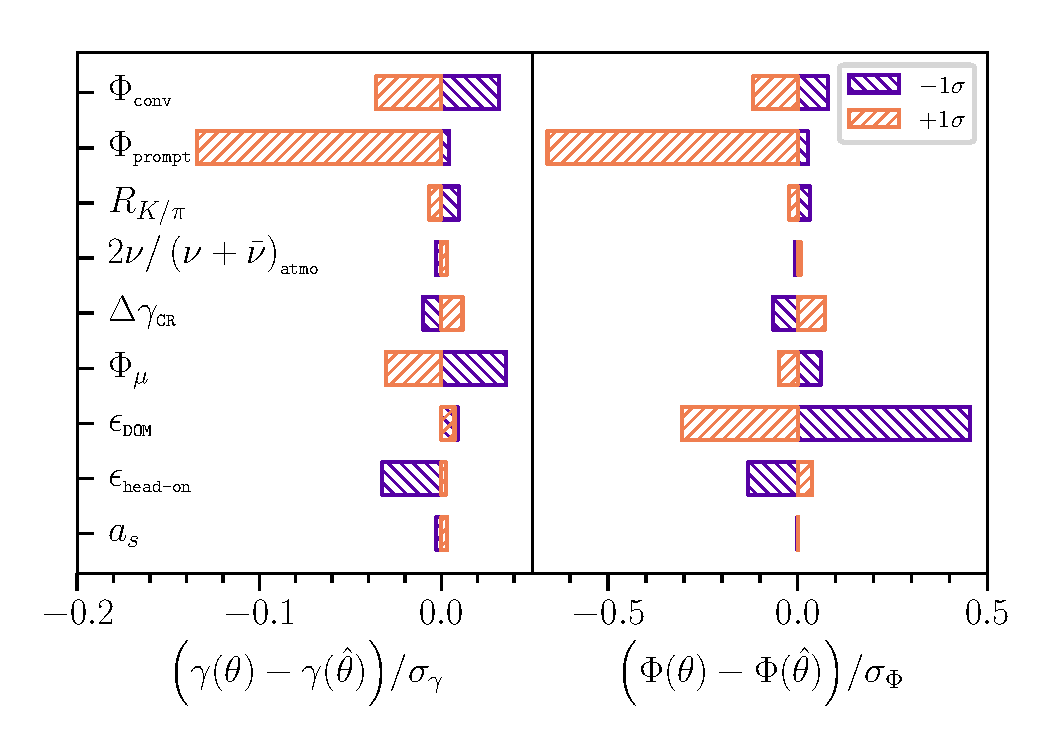
\includegraphics[width=\linewidth]{figures/hese_paper/astroDeltaGamma_astroNorm_impact}
	\internallinenumbers
	\caption{\textbf{\textit{Impact of systematic uncertainties on the single power-law parameters.}}
		Each panel shows the impact of the systematic on the astrophysical normalization (left panel) and spectral index (right panel).
		The impact, horizontal axis, is defined as the change in the parameter of interest relative to its uncertainty when modifying one systematic nuisance parameter.
		Orange bars indicate the effect of increasing the value of the nuisance parameter from its maximum {\it{}a posteriori} value by $1\sigma$ as defined by the nuisance parameter's $\SigmaOne$ highest posterior density region, while blue bars indicate the corresponding reduction of the parameter.
		Systematic parameter values are given in \reftab{tbl:spl_parameters}.
		The prompt normalization ($\promptnorm$) and DOM efficiency ($\domeff$) have the largest effect on the astrophysical parameters.
		All other systematics pull the astrophysical parameters by significantly less than $0.5\sigma$.}
	\label{fig:SPL_impacts}
\end{figure}

Our results agree with previous iterations of this analysis~\cite{Aartsen:2014gkd} within the $2\sigma$ confidence regions of the astrophysical power-law parameters.
The previous analysis obtained a best-fit spectral index of $\astrodeltagamma={2.3}^{+0.3}_{-0.3}$, compared to $\astrodeltagamma=\SPLFreqWilksIndexSummary$ in this analysis.
This difference is primarily driven by an excess(deficit) of low energy events observed in the latter $\SI{4.5}\year$(first $\SI{3}\year$).
A smaller contribution comes from the extension of the analysis energy range from $\SI{3}\PeV$ to $\SI{10}\PeV$, shifting the spectral index to a softer flux by $\sim 0.1$.
Further extension of the analysis energy range produces negligible changes.

To investigate the shift in spectral index between analysis iterations, an {\it{}a posteriori} analysis of the data time dependence was performed.
Specifically, we compared a null hypothesis of a constant flux to a time dependent spectrum with different astrophysical spectra for each of the two data partitions (first $\SI{3}\year$ and latter $\SI{4.5}\year$), where each spectrum is modeled as a single power law.
We performed a likelihood ratio based model comparison test which rejects the null hypothesis with a p-value of $\sim0.13$.
We conclude that there is no substantial evidence for time dependence in this data sample.

Additionally, we tested the effect of different systematics on the fit.
We found that the inclusion or exclusion of any individual systematic or tested combination of systematics did not appreciably affect the fit result or uncertainties.

Other crosschecks were performed with the sample: comparing the spectrum of tracks and cascades, comparing the up-going and down-going spectra, comparing the summer and winter spectra, comparing the spectra from events in different regions of the detector, comparing the charge distributions of events across a number of categorizations, comparing differences between charge calibrations, and checking for pulls resulting from reconstruction and simulation changes.
None of these checks showed any statistically significant or concerning differences.

\begin{figure}
	\centering
	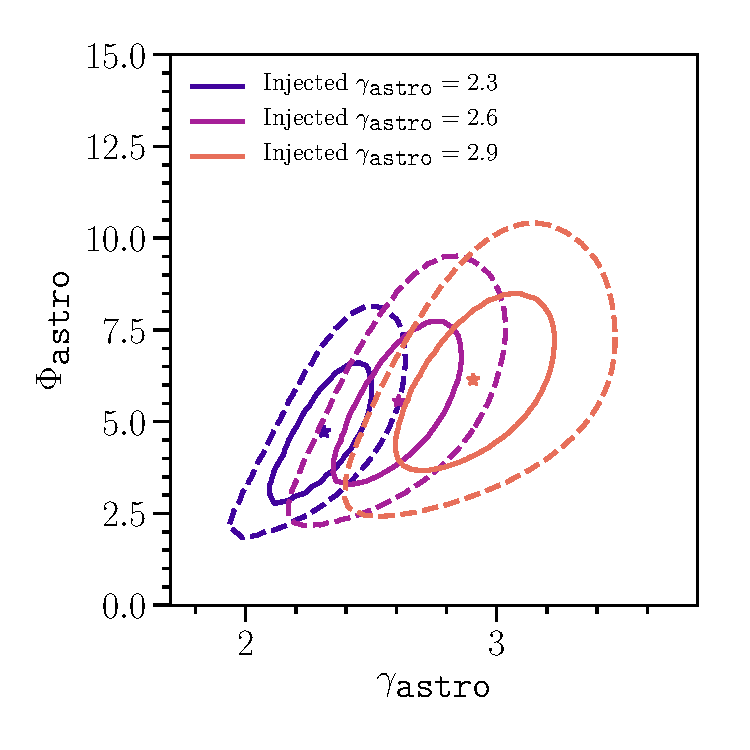
\includegraphics[width=\linewidth]{figures/hese_paper/spl_asimov_sensitivity}
	\internallinenumbers
	\caption{\textbf{\textit{Astrophysical parameter sensitivity to injected spectra.}}
		The three colors from blue to salmon show the expected astrophysical parameter $\SigmaOne$ (solid lines) and $\SigmaTwo$ (dashed lines) uncertainty for three injected astrophysical spectra $\astrodeltagamma=\{2.3, 2.6, 2.9\}$ respectively.
		In each of these cases the expected number of events for $\SI{7.5}\year$ of livetime is injected as data using nominal values for nuisance parameters and holding the number of injected astrophysical events to be equal between the spectra.
		As expected, the spectral index uncertainty grows with softer spectra from $\sim0.14$ to $\sim0.21$ when changing $\astrodeltagamma$ from $2.3$ to $2.9$.
	}
	\label{fig:SPL_asimov_sensitivity}
\end{figure}

Although the uncertainty on $\astrodeltagamma$ is numerically similar between this analysis and the $\SI{3}\year$ analysis, this is not the result of any additional systematic uncertainty or analysis change.
This is a direct result of the change in the best-fit spectral index.
Harder spectra can be measured with less uncertainty than softer spectra with the same amount of data.
This effect is shown in \reffig{fig:SPL_asimov_sensitivity} where we plot the uncertainty for different injected spectra ($\astrodeltagamma=\{2.3, 2.6, 2.9\}$) that have the same number of expected events in the sample.

Plotted in \reffig{fig:SPL_frequentist} are the confidence regions for other IceCube analyses.
The orange contours show the results of a single power-law fit to IceCube's up-going muon neutrino data sample~\cite{Stettner:2019tok}, the salmon contours show results from IceCube’s 6yr cascade sample~\cite{hansthesis}, the purple contours show results from IceCube's 5yr inelasticity measurement~\cite{Aartsen:2018vez}, and the blue contour show results from this work.
It is plain to see that there are differences in the single power-law fit results of these samples.
However, these samples cover different energies, flavors, regions of the sky, and are susceptible to different systematics and physical effects.
Differences due to these factors could help to explain the different spectral measurements and have been tested for within the samples, although presently we have not found evidence of a primary cause.
The difference may also be statistical in nature and we are continuing to investigate this point.
We briefly describe the samples for the sake of comparison.

The up-going muon neutrino sample~\cite{Stettner:2019tok}, collected over $\SI{9.5}\year$, consists of well reconstructed muon tracks with zenith angle $\theta_z \geq \SI{85}\degree$ that also pass a boosted decision tree based cut designed to select for through-going muon neutrino events while removing down-going muon and cascade backgrounds~\cite{Aartsen:2016xlq}.
This sample contains muons of energy between $\sim\SI{100}\GeV$ and $\sim\SI{10}\PeV$, with the energy distribution peaked at $\sim\SI{1}\TeV$.
Atmospheric neutrinos dominate the sample, comprising $>\SI{99}\percent$ of events in it.
The signal of astrophysical events is only apparent at the high energy range of the sample, where the atmospheric spectrum falls below the astrophysical component.
At $\sim\SI{20}\TeV$ the astrophysical component is $\sim1/10\textmd{th}$ the atmospheric component.
The components are equal in flux at $\sim\SI{200}\TeV$, and the atmospheric component is $\sim1/10\textmd{th}$ of the astrophysical component at $\sim\SI{1}\PeV$.
Events in this sample with neutrino energy between $\SI{194}\TeV$ and $\SI{7.8}\PeV$ contribute to $\SI{90}\percent$ of the total observed likelihood ratio between the best-fit and the atmospheric-only hypothesis.
As a function of the zenith angle, the signal to background ratio is lower at the horizon than for up-going events by almost an order of magnitude because of the enhanced atmospheric neutrino production at the horizon.

The cascade neutrino sample, collected over six years, consists of cascade-like events from all directions in the sky that have neutrino energies between $\sim\SI{1}\TeV$ and $\sim\SI{10}\PeV$.
Above $\SI{60}\TeV$ this sample is largely composed of events also contained in the HESE sample.
As the sample selects for cascade-like events, it predominantly contains electron and tau neutrinos, but also contains neutral current events from all neutrino flavors and a fraction of misidentified muon neutrinos.
We can attribute $\SI{90}\percent$ of the total observed likelihood ratio between the best-fit and the atmospheric-only hypothesis to events with neutrino energy between $\SI{12}\TeV$ and $\SI{2.1}\PeV$.
The distribution of the signal to background ratio is more complicated for this sample, ranging from 1:100 at $\si\TeV$ energies to 1000:1 at $\si\PeV$ energies.
The sample is least pure near the horizon with a factor of 10 to 100 less signal per background compared to the up-going and down-going regions.

The sample used for the inelasticity measurement, collected over five years, consists of track and cascade events with their interaction vertex contained within the detector. The sample is optimized to facilitate the measurement of the neutrino interaction inelasticity distribution, using both a veto and boosted decision tree to select neutrino events while removing atmospheric muons. The sample is sensitive in the $\SI{1}\TeV$ to $\SI{1}\PeV$ energy range with the bulk of events below $\SI{10}\TeV$. Signal to background ratios of 10:1 are achieved for tracks close to $\SI{1}\PeV$ and cascades above $\SI{100}\TeV$. Up-going track events in this sample are a factor of 10 to 1000 more pure than down-going track events and a factor of 10 to 100 more pure for cascades.

In contrast to these samples, the HESE selection which is the focus of this work has a similar effective area for all neutrino flavors and a signal to background profile with features closer to the cascade sample.
Events in this sample with neutrino energy between $\SI{69.4}\TeV$ and $\SI{1.9}\PeV$ contribute $\SI{90}\percent$ of the total observed likelihood ratio between the best-fit and the atmospheric-only hypothesis.
Above $\SI{60}\TeV$ deposited energy, the sample has 60 events with signal to background ratio greater than 1:10 , 59 events with signal to background ratio greater than 1:1, 24 events with signal to background ratio greater than 10:1, 10 events with signal to background ratio greater than 100:1, 3 events with signal to background ratio greater than 1000:1, and 1 event with signal to background ratio greater than 10000:1.
This variation in signal to background ratio stems both from the differing spectra of the fluxes, and the varying rejection power of the veto with respect to the zenith angle.

HESE and the through-going muon neutrino sample have comparable sensitivity to the energy spectrum under the single power-law assumption when one accounts for the parameter-space differences between the best-fit spectral indices as demonstrated in \reffig{fig:SPL_asimov_sensitivity}.
The HESE sample suffers from small sample size but benefits from high astrophysical purity, while the through-going muon neutrino sample benefits from large sample size but suffers from lower purity and worse energy resolution of tracks.
The cascade and inelasticity selections have comparable spectral sensitivity to each other that is better than the other two samples.
Both benefit from large sample size; the cascade sample and inselasticity sample benefit from the better resolution of cascades and starting tracks respectively.

Assuming a continuous single power law across all energies, the large gamma values of the preferred regions in this analysis are disfavored by the through-going muon and cascade sample results.
As the samples are sensitive to different types of events when measuring the astrophysical flux, the differences between the spectral measurements may be attributable to spectral features, large-scale anisotropy, flavor differences, or other alternatives.
At this stage the exact cause of the differing results is not immediately clear, but the results agree within their $\SigmaTwo$ confidence regions.

% SPl parameter information
\begin{figure}
	\centering
	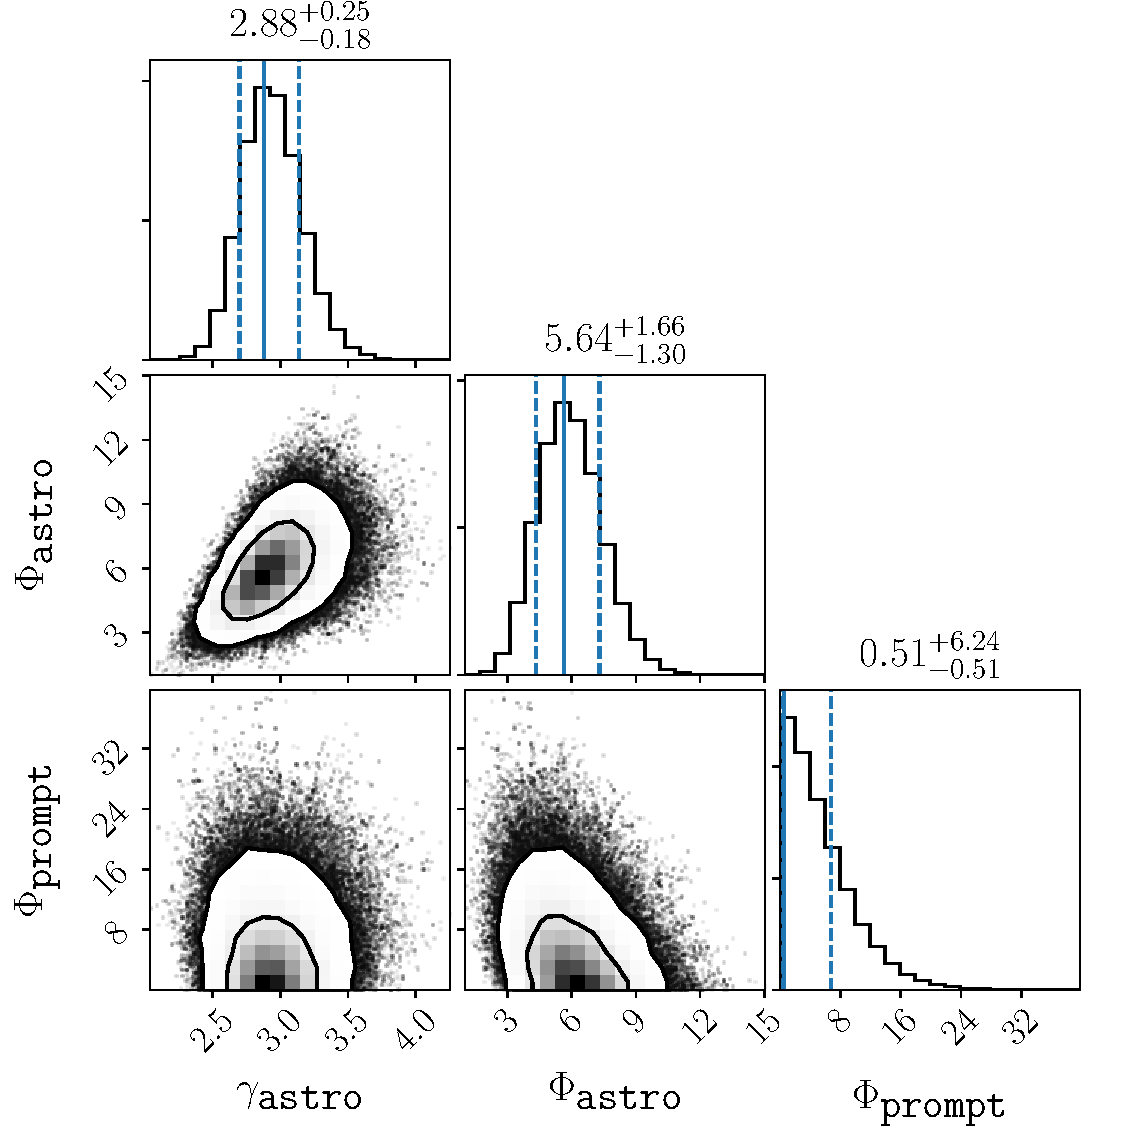
\includegraphics[width=\linewidth]{figures/hese_paper/spl_posterior}
	\internallinenumbers
	\caption{\textbf{\textit{Single power-law parameters posteriors.}}
		Diagonal panels show the one-dimensional posterior distribution of the parameters (joint distribution integrated over all other parameters), where the horizontal axis of the panel is the same as the horizontal axis at the bottom of the column, and the vertical axis of the panel is the probability density in arbitrary scale.
		The solid blue lines denote the MAP estimator for each parameter, and the dashed lines denote the bounds of the one-dimensional $\SigmaOne$ HPD region, these numbers are also listed above the diagonal panels.
		Non-diagonal panels show the two-dimensional posterior distribution of the parameters, where the horizontal and vertical axes of the panel correspond to the horizontal axis at the bottom of the column and the vertical axis at the far left of the row respectively.
		The innermost contours show the two-dimensional $\SigmaOne$ HPD region and the outermost contours show the $\SigmaTwo$ HPD region.
		The color scale of the histogram within the contours shows the probability density in arbitrary scale.
		The points outside of the contours show individual points from the MCMC.}\label{fig:SPL_posterior}
\end{figure}

A Bayesian analysis was also performed assuming a single power-law model for the astrophysical spectrum.
We examine the posterior distribution which is a product of the likelihood and the priors, integrated over the nuisance parameters.
In \reftab{tbl:spl_parameters} for each parameter we report the maximum {\it{}a posteriori} (MAP) estimation of the variable, as well as the $\SigmaOne$ highest posterior density (HPD) region.
The parameters of the SPL model were found to be compatible when assuming improper uniform priors in linear parameter space or in the logarithm of the parameters.
We obtain a most likely spectral index of $\astrodeltagamma=\SPLBayesIndexSummary$, in excellent agreement with the frequentist estimation of these parameters, implying that the MAP is dominated by the data rather than the priors of the SPL parameters.
%and that there is not a strong bias from variables correlated with the spectral index.
\reffig{fig:SPL_posterior} shows one-dimensional projections of the posterior distribution on the diagonal, integrated over the other variables, with the $\SigmaOne$ HPD region bounds plotted as vertical lines.
The non-diagonal panels of \reffig{fig:SPL_posterior} show contours of the $\SigmaOne$ and $\SigmaTwo$ HPD regions of the two-dimensional posterior distribution projection.
Within the contours a histogram of the probability is displayed, and outside the contours individual samples from the MCMC are plotted.
One can see the correlation between $\astrodeltagamma$ and $\astronorm$; this correlation arises because the overall normalization of events must be roughly preserved in order to match the data well.
Additionally the inverse correlation of $\astronorm$ and $\promptnorm$ is apparent in this figure, which also arises from a conserved total number of events.
%TODO add more about the prompt being compatible with zero
Both the Bayesian and frequentist analyses show $\promptnorm$ to be compatible with zero.

\begin{table*}[thb]
	\centering
	\begin{tabular}{l rr rr}
		Parameter & \multicolumn{2}{c }{Frenquentist Analysis} & \multicolumn{2}{c}{Bayesian Analysis} \\
		\toprule
		& Best-fit value & $\SigmaOne$ C.L. & Most-likely value & $\SigmaOne$ H.P.D. \\
		\midrule
		\multicolumn{1}{l }{\textbf{Astrophysical neutrino flux:}} & & & &\\
		$\astronorm$ & $\SPLFreqBFNorm$ & $[\SPLFreqWilksLowerNorm,\SPLFreqWilksUpperNorm]$ & $\SPLBayesMAPNorm$ & $[\SPLBayesHPDLowerNorm,\SPLBayesHPDUpperNorm]$\\
		$\astrodeltagamma$ & $\SPLFreqBFIndex$ & $[\SPLFreqWilksLowerIndex,\SPLFreqWilksUpperIndex]$ & $\SPLBayesMAPIndex$ & $[\SPLBayesHPDLowerIndex,\SPLBayesHPDUpperIndex]$\\
		\midrule
		\multicolumn{1}{l }{\textbf{Atmospheric neutrino flux:}} & & & &\\
		$\convnorm$ & $\SPLFreqBFConvNorm$ & $[\SPLFreqWilksLowerConvNorm,\SPLFreqWilksUpperConvNorm]$ & $\SPLBayesMAPConvNorm$ & $[\SPLBayesHPDLowerConvNorm,\SPLBayesHPDUpperConvNorm]$\\
		$\promptnorm$ & $\SPLFreqBFPromptNorm$ & $[\SPLFreqWilksLowerPromptNorm,\SPLFreqWilksUpperPromptNorm]$ & $\SPLBayesMAPPromptNorm$ & $[\SPLBayesHPDLowerPromptNorm,\SPLBayesHPDUpperPromptNorm]$\\
		$\pik$ & $\SPLFreqBFKPi$ & $[\SPLFreqWilksLowerKPi,\SPLFreqWilksUpperKPi]$ & $\SPLBayesMAPKPi$ & $[\SPLBayesHPDLowerKPi,\SPLBayesHPDUpperKPi]$\\
		$\atmonunubar$ & $\SPLFreqBFAtmoNuRatio$ & $[\SPLFreqWilksLowerAtmoNuRatio,\SPLFreqWilksUpperAtmoNuRatio]$ & $\SPLBayesMAPAtmoNuRatio$ & $[\SPLBayesHPDLowerAtmoNuRatio,\SPLBayesHPDUpperAtmoNuRatio]$\\
		\midrule
		\multicolumn{1}{l }{\textbf{Cosmic ray flux:}} & & & & \\
		$\crdeltagamma$ & $\SPLFreqBFCRDeltaGamma$ & $[\SPLFreqWilksLowerCRDeltaGamma,\SPLFreqWilksUpperCRDeltaGamma]$ & $\SPLBayesMAPCRDeltaGamma$ & $[\SPLBayesHPDLowerCRDeltaGamma,\SPLBayesHPDUpperCRDeltaGamma]$\\
		$\muonnorm$ & $\SPLFreqBFMuonNorm$ & $[\SPLFreqWilksLowerMuonNorm,\SPLFreqWilksUpperMuonNorm]$ & $\SPLBayesMAPMuonNorm$ & $[\SPLBayesHPDLowerMuonNorm,\SPLBayesHPDUpperMuonNorm]$\\
		\midrule
		\multicolumn{1}{l }{\textbf{Detector:}} & & & &\\
		$\domeff$ & $\SPLFreqBFDOMEff$ & $[\SPLFreqWilksLowerDOMEff,\SPLFreqWilksUpperDOMEff]$ & $\SPLBayesMAPDOMEff$ & $[\SPLBayesHPDLowerDOMEff,\SPLBayesHPDUpperDOMEff]$\\
		$\holeice$ & $\SPLFreqBFHoleIce$ & $[\SPLFreqWilksLowerHoleIce,\SPLFreqWilksUpperHoleIce]$ & $\SPLBayesMAPHoleIce$ & $[\SPLBayesHPDLowerHoleIce,\SPLBayesHPDUpperHoleIce]$\\
		$a_s$ & $\SPLFreqBFAniScale$ & $[\SPLFreqWilksLowerAniScale,\SPLFreqWilksUpperAniScale]$ & $\SPLBayesMAPAniScale$ & $[\SPLBayesHPDLowerAniScale,\SPLBayesHPDUpperAniScale]$\\
		\bottomrule
	\end{tabular}
	\internallinenumbers
	\caption{\textbf{\textit{Single power-law model parameters.}} The frequentist analysis column shows the best-fit parameters and their corresponding $\SigmaOne$ C.L. interval according to Wilks' theorem for the single power-law model.
		The Bayesian analysis column shows the most-likely values of the parameters as well as the $\SigmaOne$ highest probability density (HPD) interval.
		Parameter name descriptions and priors(constraints) are given in \reftab{tbl:priors}.}
	\label{tbl:spl_parameters}
\end{table*}

\subsubsection{Double power-law flux\label{sec:dpl}}

\noindent
\textit{%Here we describe the double power-law model analysis.
	This model can be parameterized as hard and soft power-law components.
	We find that the preferred value of the hard component spectral index is close to that of the single power-law result, \textit{i.e.} $\gamma_\texttt{hard} \sim 2.8$ and $\gamma_\texttt{astro} \sim 2.9$, while the soft component spectral index most-likely value is $\gamma_\texttt{soft} \sim 3.1$.
	The latter is poorly constrained and values as large as $\gamma_\texttt{soft}=3.4$ are contained within the $\SigmaOne$ highest probability density region.
	The normalizations of the two components are highly correlated, with either equal to zero allowed within the $\SigmaTwo$ highest probability density region.
	This observation is aligned with our conclusion that there is no statistical significance for an additional power-law component in this sample.
}
\newline

The double power law is an extension to the single power law, which introduces a second power-law component with duplicated free parameters.
In this model the astrophysical differential flux is described as
\begin{linenomath*}
	\begin{equation}
	\begin{split}
	&\frac{d\Phi_{6\nu}}{dE} = \\
	&\left(\Phi_\texttt{astro1}{\left(\frac{E_\nu}{\SI{100}\TeV}\right)}^{-\gamma_\texttt{astro1}}\right. + \left. \Phi_\texttt{astro2}{\left(\frac{E_\nu}{\SI{100}\TeV}\right)}^{-\gamma_\texttt{astro2}}\right) \\
	& \cdot 10^{-18}~[\textmd{GeV}^{-1}\textmd{cm}^{-2}\textmd{s}^{-1}\textmd{sr}^{-1}].
	\end{split}
	\label{eq:dpl_flux}
	\end{equation}
\end{linenomath*}

The astrophysical parameters of this model are then $\Phi_\texttt{astro1}$, $\Phi_\texttt{astro2}$, $\gamma_\texttt{astro1}$, and $\gamma_\texttt{astro2}$ which adds two more parameters compared to the single power law.
The functional form of this model means that it is equivalent to the single power-law model when $\Phi_\texttt{astro1}$ or $\Phi_\texttt{astro2}$ become zero or when $\gamma_\texttt{astro1}=\gamma_\texttt{astro2}$.
We choose improper uniform priors for the astrophysical model where the parameters are restricted to be positive, as was done for the single power law.
There is implicitly a degeneracy of the parameters in the model.
For the purpose of sampling the posterior distribution this degeneracy is not an issue, however it is more informative to construct some parameters that break the degeneracy and examine the posterior distribution in those new variables.
We define
\begin{linenomath*}
	\begin{equation}
	\begin{split}
	\gamma_\texttt{hard} &= \min (\gamma_\texttt{astro1}, \gamma_\texttt{astro2}), \\
	\gamma_\texttt{soft} &= \max (\gamma_\texttt{astro1}, \gamma_\texttt{astro2}), \\
	\Phi_\texttt{hard} &= \left\{ \begin{array}{ll} \Phi_\texttt{astro1} & \gamma_\texttt{astro1} \leq \gamma_\texttt{astro2} \\ \Phi_\texttt{astro2} & \gamma_\texttt{astro1} > \gamma_\texttt{astro2} \end{array} \right. , \\
	\Phi_\texttt{soft} &= \left\{ \begin{array}{ll} \Phi_\texttt{astro2} & \gamma_\texttt{astro1} \leq \gamma_\texttt{astro2} \\ \Phi_\texttt{astro1} & \gamma_\texttt{astro1} > \gamma_\texttt{astro2} \end{array} \right. ,
	\end{split}\label{eq:dpl_hardsoft}
	\end{equation}
\end{linenomath*}
to split the parameters into a hard component and soft component.
These parameters are used to display the posterior distribution in \reffig{fig:dpl_posterior} in the same manner as we did for the single power-law parameters.
% TODO Describe interesting features of the plot
In \reffig{fig:dpl_posterior} the normalizations of the two components are seen to be anti-correlated as an astrophysical component is required by the data, but both normalizations are compatible with zero within the two-dimensional $\SigmaOne$ HPD region of the joint normalization posterior distribution.
This indicates that two power-law components are not strongly preferred over a single power-law component.

% DPL parameter information
\begin{figure}
	\centering
	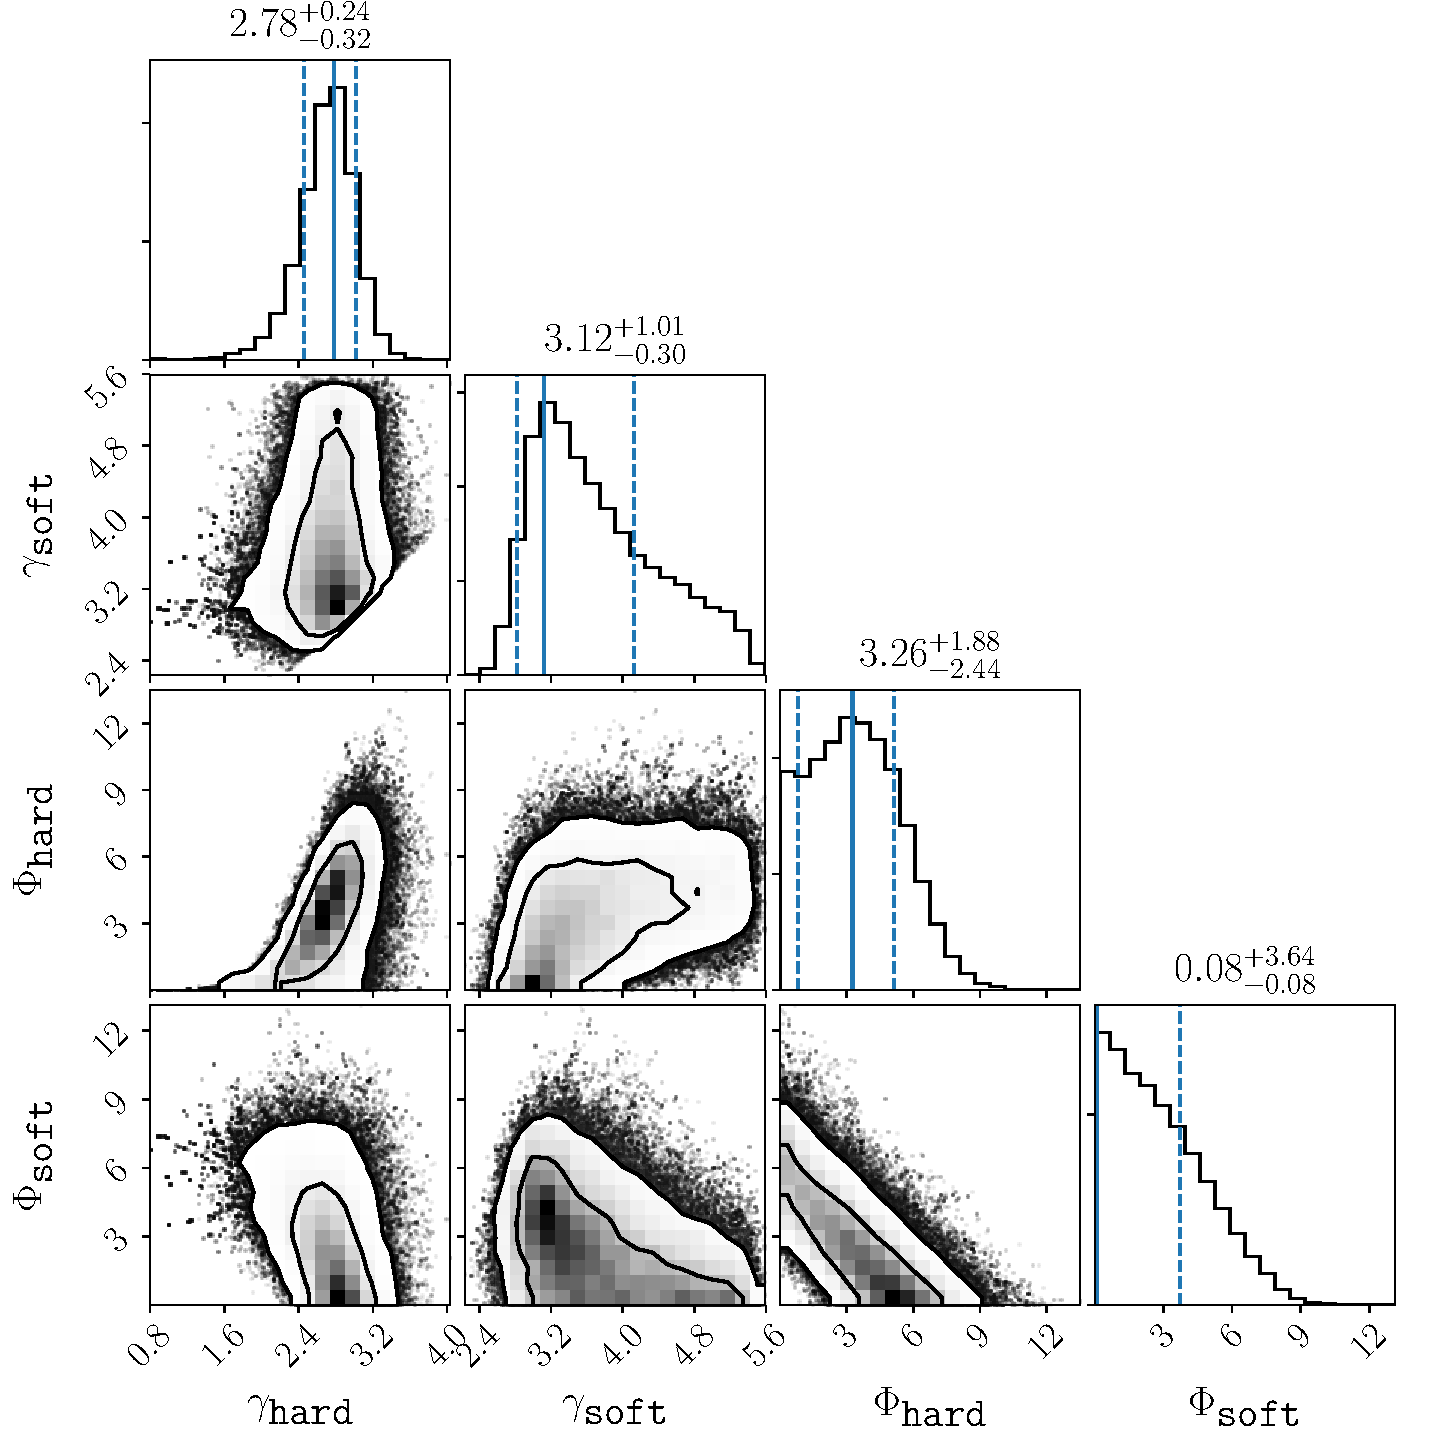
\includegraphics[width=\linewidth]{figures/hese_paper/dpl_flat_hardsoft_vars}
	\internallinenumbers
	\caption{\textbf{\textit{Double power-law model hard/soft parameters posterior distribution.}}
		Results derived from the posterior distribution of the model are shown in the same style as \reffig{fig:SPL_posterior}.
		The figure shows the one- and two-dimensional posterior distributions for the parameters of the hard and soft components of the astrophysical neutrino flux.
		The diagonal panels show the one-dimensional posterior with the parameter MAP estimation and $\SigmaOne$ HPD region indicated, while the non-diagonal panels show the two-dimensional posterior with $\SigmaOne$ and $\SigmaTwo$ regions indicated.}\label{fig:dpl_posterior}
\end{figure}

As there are two regions of parameter space where the this model is equivalent to a single power law we construct another set of variables to understand the behavior of the model
\begin{linenomath*}
	\begin{equation}
	\begin{split}
	\Delta\gamma_\texttt{astro} &= \gamma_\texttt{soft} - \gamma_\texttt{hard}, \\
	\Delta\Phi_\texttt{astro} &= \Phi_\texttt{soft} - \Phi_\texttt{hard}.
	\end{split}\label{eq:dpl_delta}
	\end{equation}
\end{linenomath*}
\reffig{fig:dpl_delta_posterior} shows that $\Delta\gamma_\texttt{astro}$ is compatible with zero, meaning again that the data is compatible with a single power law in this model.

% DPL delta parameter information
\begin{figure}
	\centering
	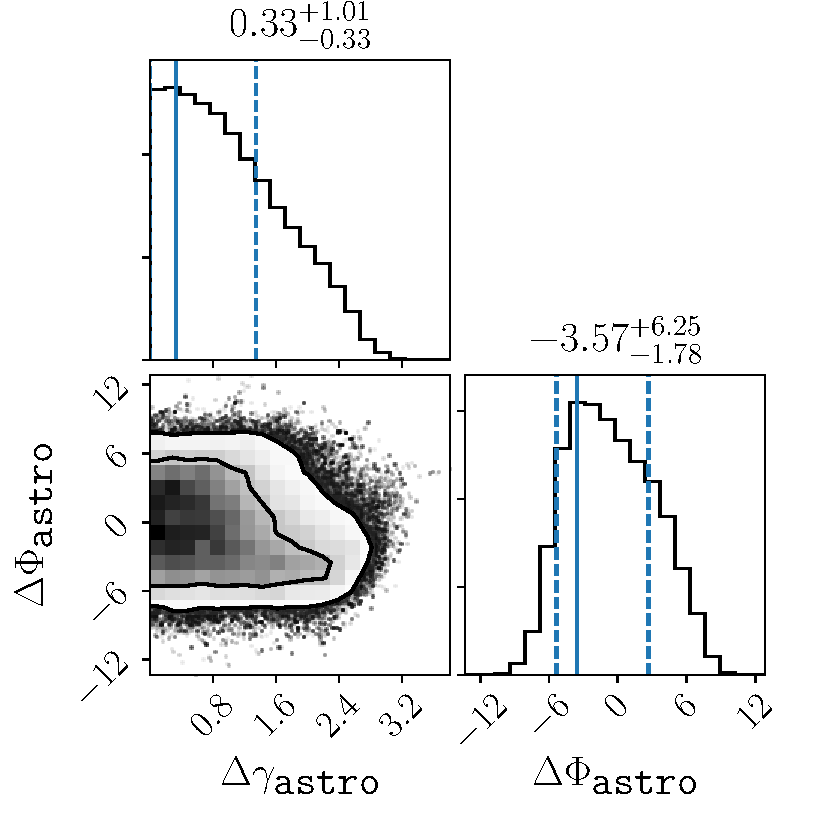
\includegraphics[width=\linewidth]{figures/hese_paper/dpl_flat_delta_vars}
	\internallinenumbers
	\caption{\textbf{\textit{Double power-law model parameter deltas posterior distribution.}}
		Results derived from the posterior distribution of the model are shown in the same style as \reffig{fig:SPL_posterior}.
		The figure shows the one- and two-dimensional posterior distributions for the difference between the parameters of the hard and soft components of the astrophysical neutrino flux.
		The diagonal panels show the one-dimensional posterior with the parameter MAP estimation and $\SigmaOne$ HPD region indicated, while the non-diagonal panel shows the two-dimensional posterior with $\SigmaOne$ and $\SigmaTwo$ regions indicated.}\label{fig:dpl_delta_posterior}
\end{figure}

\subsubsection{Single power law with spectral cutoff\label{sec:cutoff}}

\noindent
\textit{%Here we report the results of a search for a spectral cutoff in this sample.
	A spectral cutoff is connected to the highest energies that the sources producing neutrinos can achieve.
	We have performed a model comparison analysis between the single power-law model without a cutoff and one with a cutoff.
	We find that models that include a cutoff with values smaller than $\sim\SI{400}\TeV$ are strongly disfavored with respect to the no-cutoff hypothesis due to the  large number of lower energy events.
	Models with cutoff energy above $\sim\SI{2}\PeV$ have evidence close to or greater than the no-cutoff hypothesis, but are not substantially favored as the sample has no events above $\sim\si\PeV$ energies.
}
\newline

The flux of the astrophysical component is given as
\begin{linenomath*}
	\begin{equation}
	\begin{split}
	\frac{d\Phi_{6\nu}}{dE}={}&\Phi_\texttt{astro}{\left(\frac{E_\nu}{\SI{100}\TeV}\right)}^{-\gamma_\texttt{astro}} \\ & \cdot e^{-\frac{E_{\nu}}{E_\texttt{cutoff}}} \\ & \cdot 10^{-18}[\textmd{GeV}^{-1}\textmd{cm}^{-2}\textmd{s}^{-1}\textmd{sr}^{-1}].
	\end{split}\label{eq:cutoff_flux}
	\end{equation}
\end{linenomath*}

To study the preference between cutoff scenarios we compute the Bayes factor for many values of the cutoff energy $E_\texttt{cutoff}$ where the null hypothesis is the single power-law model and the alternative hypothesis is the cutoff model.
The Bayes factor in this case is defined as
\begin{linenomath*}
	\begin{equation}
	\begin{split}
	\mathcal{B}(E_\texttt{\small{cutoff}}) ={}& \frac{\int d\vec\eta~\mathcal{L}_\texttt{\tiny{cutoff}}(E_\texttt{\tiny{cutoff}},\vec\eta)\cdot\Pi(\vec\eta)}{\int d\vec\eta~\mathcal{L}_\texttt{\tiny{SPL}}(\vec\eta)\cdot\Pi(\vec\eta)},
	\end{split}\label{eq:cutoff_bayes_factor}
	\end{equation}
\end{linenomath*}
where $\mathcal{L}_\texttt{\tiny{cutoff}}$ is the likelihood of the cutoff model, $\mathcal{L}_\texttt{\tiny{SPL}}$ is the likelihood of the single power-law model, and $\Pi$ is the set of priors given in \reftab{tbl:priors}.
\reffig{fig:cutoff_bayes} shows the inverse of the Bayes factor $\mathcal{B}$ as a function of $E_\texttt{cutoff}$.
For most values of $E_\texttt{cutoff}$ the Bayes factor is less than one, this implies that the data in this sample favors a model with no cutoff in most cases.
For regions where $\mathcal{B} < 1$ we can exclude values of the cutoff with some level of certainty.
\reffig{fig:cutoff_bayes} shows excluded regions of the cutoff chosen according to Jeffreys' scale.

In addition to the Bayes factor treatment described above, we also perform a test using a frequentist test-statistic, defined as
\begin{linenomath*}
	\begin{equation}
	\begin{split}
	\TS(E_\texttt{\small{cutoff}}) ={}& -2\log\left({\frac{\max_{\vec\eta}\mathcal{L}_\texttt{\tiny{cutoff}}(E_\texttt{\tiny{cutoff}},\vec\eta)\cdot\Pi(\vec\eta)}{\max_{\vec\eta}\mathcal{L}_\texttt{\tiny{SPL}}(\vec\eta)\cdot\Pi(\vec\eta)}}\right),
	\end{split}\label{eq:cutoff_ts}
	\end{equation}
\end{linenomath*}
in order to compare to other IceCube measurements of a spectral cutoff.
The null hypothesis as before is the single power-law model, and the alternative hypothesis is the spectral cutoff model with the cutoff energy as a free parameter.
This model-comparison test rejects the null-hypothesis with a p-value of $0.66$.
To further visialize the cutoff energy parameter space favored or disfavored, we plot the test statistic as a function of the cutoff energy in \reffig{fig:cutoff_freq}.
Cutoff energies below $\sim\SI{1}\PeV$ are disfavored at more than the $\SigmaOne$ confidence level, while cutoff energies above this including the no cutoff scenario are compatible within the $\SigmaOne$ confidence level.

% Cutoff bayes factor plot
\begin{figure}
	\centering
	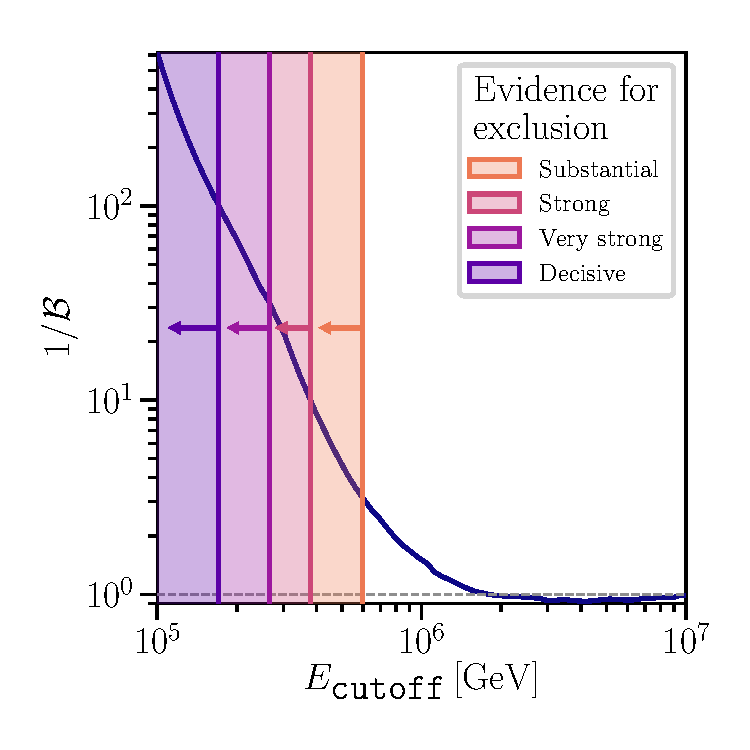
\includegraphics[width=\linewidth]{figures/hese_paper/cutoff_bayes}
	\internallinenumbers
	\caption{\textbf{\textit{Spectral cutoff Bayes factors and regions of exclusion.}}
		The inverse of the Bayes factor, $\mathcal{B}$, is plotted in the blue curve as a function of the cutoff energy assumed in the alternative hypothesis.
		Regions of the cutoff energy shown by the shaded regions are disfavored with respect to the null hypothesis with varying degrees of certainty according to Jeffreys' scale.
		The Bayes factor is computed for each value of the cutoff energy with the single power-law as a null hypothesis.
		The grey dashed line indicates where the evidence of the cutoff model and the single power-law model are equal.}\label{fig:cutoff_bayes}
\end{figure}

\begin{figure}
	\centering
	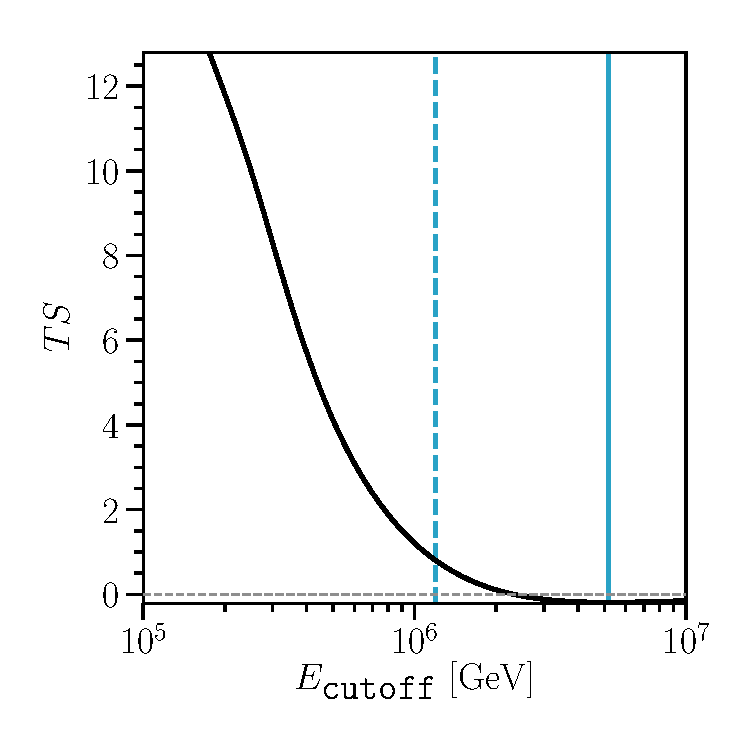
\includegraphics[width=\linewidth]{figures/hese_paper/cutoff_freq}
	\internallinenumbers
	\caption{\textbf{\textit{Cutoff model comparison using frequentist test-statistic.}}
		The test-statistic comparing the cutoff hypothesis and the single power-law hypothesis is plotted as the black curve.
		We also report in the plot the best-fit value for the cutoff energy, $E_\texttt{cutoff}$, as the solid blue line and its $\SigmaOne$ confidence interval as the dashed blue line.
		The grey dashed line indicates where the test-statistic of the cutoff model and the single power-law model are equal.}\label{fig:cutoff_freq}
\end{figure}

\subsubsection{Log-parabola flux\label{sec:log_parabola}}

\noindent
\textit{%Here we consider the possibility that the spectral index varies logarithmically with respect to the neutrino energy.
	This model has two relevant parameters: the spectral index at the $\SI{100}\TeV$ pivot point and the spectral index rate of change.
	In this model, the spectral index at the pivot point and the spectral index rate of change are simultaneously compatible with the single power-law spectral index and zero respectively.
	This implies that in the measured energy range we observe no indication of log-linear spectral change.
}
\newline

In log-energy log-flux space the single power law can be represented as a line.
A simple functional extension is to add curvature to this line, this is the log-parabola model which has the form

\begin{linenomath*}
	\begin{equation}
	\begin{split}
	\frac{d\Phi_{6\nu}}{dE}={}&\Phi_\texttt{astro}{\left(\frac{E_\nu}{\SI{100}\TeV}\right)}^{-\left(\alpha+\beta \log(\frac{E_\nu}{\SI{100}\TeV})\right)} \\ & \cdot 10^{-18}[\textmd{GeV}^{-1}\textmd{cm}^{-2}\textmd{s}^{-1}\textmd{sr}^{-1}],
	\end{split}\label{eq:logparabola_flux}
	\end{equation}
\end{linenomath*}
where $\alpha$ is the spectral index at $\SI{100}\TeV$, and $\beta$ governs how the effective spectral index changes with energy.
In the Bayesian analysis of this model, we have chosen improper uniform priors for both $\alpha$ and $\beta$.
At $\SI{100}\TeV$ the most-likely spectral index ($\alpha=2.78$) is still soft, and compatible with the most-likely SPL spectral index ($\astrodeltagamma=\SPLBayesMAPIndex$) within the $\SigmaOne$ HPD region of $\alpha$.
There is one region of the parameter space where the log-parabola model becomes the same as a single power law, when $\beta=0$.
This region of parameter space is within the $\SigmaOne$ HPD region of $\beta$, informing us that the data is most compatible with a model that is close to a single power law rather than a model with larger curvature.

% Log parabolic small corner plot
\begin{figure}
	\centering
	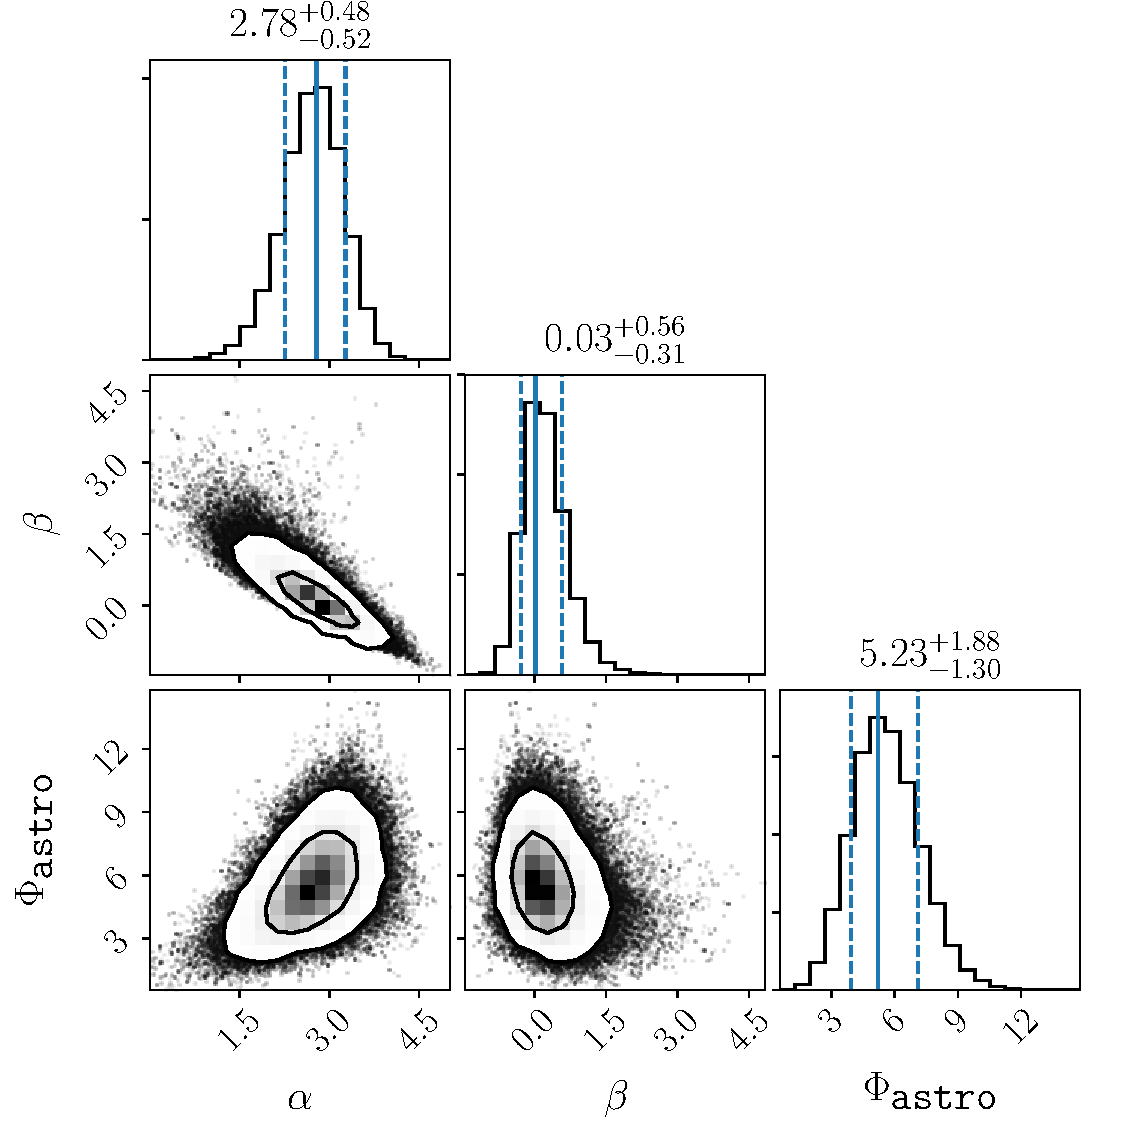
\includegraphics[width=\linewidth]{figures/hese_paper/lppl}
	\internallinenumbers
	\caption{\textbf{\textit{Log-parabola astrophysical model parameters posterior distribution.}}
		Results derived from the posterior distribution of the model are shown in the same style as \reffig{fig:SPL_posterior}.
		The figure shows the one- and two-dimensional posterior distributions for the astrophysical flux normalization, $\astronorm$; the spectral index at $\SI{100}\TeV$, $\alpha$; and the change in spectral index, $\beta$.
		The diagonal panels show the one-dimensional posterior with the parameter MAP estimation and $\SigmaOne$ HPD region indicated, while the non-diagonal panels show the two-dimensional posterior with $\SigmaOne$ and $\SigmaTwo$ regions indicated.
		As we can see from the posterior distribution, $\beta$ is compatible with zero which implies that an unbroken power law is a good fit to the data under under these model constraints.}\label{fig:log_parabola_powerlaw_corner}
\end{figure}

%Log paraboloid

\subsubsection{Segmented power-law flux\label{sec:unfolding}}

\noindent
\textit{The neutrino spectrum can be generically parameterized as a set of narrow $E^{-2}$ power-law segments.
	We report the normalization of each of these segments and their uncertainties.
	It is notable that the energy density of the two lowest energy segments is higher than the five highest energy segments by a factor of $\sim 2-3$.
	The origin of this increase also drives the soft spectrum observed in the single power law model.
	This suggests the existence of gamma-opaque sources that dominate the flux at the lowest energies if the trend continues~\cite{Murase:2015xka,Ando:2015bva,Bechtol:2015uqb,Meszaros:2017fcs}.
}
\newline

The models explored in previous sections restrict the spectrum to be described by an unbroken power-law-like model across the entire energy range.
In this section, we introduce a model that is a more general parameterization of the astrophysical flux.
We split the neutrino energy spectrum into segments equally spaced in $\log E_\nu$, assume an $E^{-2}$ spectrum within each segment, and then allow the normalizations of each segment to vary independently.
This model, while not entirely general, is able to describe a wide variety fluxes within the current detector energy resolution.
In this work we use a segmented model in which the astrophysical neutrino flux within each segment is given by
\begin{linenomath*}
	\begin{align}
	\begin{split}
	\frac{d\Phi_{6\nu}}{dE} ={}& \Phi_{i} {\left(\frac{E_\nu}{E_{c,i}}\right)}^{-2}\\
	& \cdot 10^{-18}[\textmd{GeV}^{-1}\textmd{cm}^{-2}\textmd{s}^{-1}\textmd{sr}^{-1}],
	\label{eq:segmented_flux}
	\end{split}
	\end{align}
\end{linenomath*}
where $\Phi_i$ is the normalization constant for each bin, $E_{c,i}$ is the log-center of each bin, and the bins span between $\SI{19.95}\TeV$ and $\SI{316.2}\PeV$.
We analyze this model in the same way as previous analyses~\cite{Aartsen:2014gkd,Aartsen:2015zva,Aartsen:2017mau}.
Namely, we obtain the best-fit point for the normalizations, which are plotted for seven energy segments (enumerated in \reftab{tbl:segment_normalizations}) in the left panel of \reffig{fig:segmented}; five other energy segments are profiled over and not shown as they are poorly constrained by the data, and do not provide significant information.
In such a high-dimensional parameter space it is computationally prohibitive to find the one-dimensional confidence intervals, which requires computing the profile likelihood at a large number of points in the parameter space.
This computational difficulty stems from the presence of many local minima.
Instead, the errors are estimated by fixing all parameters except one normalization, and finding the range of this normalization for which $\Delta\max_{\vec\eta}\like\cdot\Pi\leq 0.5$.
This corresponds to an approximate one-dimensional $\SigmaOne$ confidence interval, with the caveat that this procedure may underestimate the errors on each segment compared to the profile likelihood technique.
As a complement to the aforementioned frequentist approach, we also analyze this model in a Bayesian way.
Assuming improper positive uniform priors for the normalizations of the power-law segments, we sample the posterior distribution of the model.
The right panel of \reffig{fig:segmented} shows the one-dimensional MAP estimation of each normalization independently for the same seven energy segments as before; the remaining five energy segments have been marginalized over as the data does not significantly constrain them.
Errors of each normalization are constructed by integrating the joined distribution over all other parameters and then computing the $\SigmaOne$ HPD region of that segment.
These errors account for correlations between normalization segments, but the one-dimensional MAP estimators cannot be considered simultaneously as a thirteen-dimensional MAP.
The one-dimensional posterior density is also plotted as a turquoise band to demonstrate the shape of the distribution, although the relative scale between bands is arbitrary.
Finally, in \reftab{tbl:segment_normalizations} the normalizations of the segments are reported for both the frequentist and Bayesian analysis.

\begin{table*}[thb]
	\centering
	\begin{tabular}{l rr rr}
		Energy Range & \multicolumn{2}{c}{Frenquentist Analysis} & \multicolumn{2}{c}{Bayesian Analysis} \\
		\toprule
		& Best-fit value & $\SigmaOne$ C.L. & Most-likely value & $\SigmaOne$ H.P.D. \\
		\midrule
		$[4.20\cdot 10^{4}, 8.83\cdot 10^{4}]$ & $5.68 \cdot 10^{-13}$ & $[-5.31, +6.57]$  & $8.18 \cdot 10^{-13}$ & $[-6.52, +8.35]$  \\
		$[8.83\cdot 10^{4}, 1.86\cdot 10^{5}]$ & $5.79 \cdot 10^{-13}$ & $[-1.25, +1.42]$  & $5.32 \cdot 10^{-13}$ & $[-1.73, +1.68]$  \\
		$[1.86\cdot 10^{5}, 3.91\cdot 10^{5}]$ & $3.22 \cdot 10^{-14}$ & $[-3.22, +4.24]$  & $1.53 \cdot 10^{-14}$ & $[-1.53, +6.18]$  \\
		$[3.91\cdot 10^{5}, 8.23\cdot 10^{5}]$ & $6.12 \cdot 10^{-15}$ & $[-6.12, +18.0]$ & $1.13 \cdot 10^{-15}$ & $[-1.12, +27.0]$  \\
		$[8.23\cdot 10^{5}, 1.73\cdot 10^{6}]$ & $1.71 \cdot 10^{-14}$ & $[-0.845, +1.14]$ & $1.14 \cdot 10^{-14}$ & $[-0.997, +1.21]$ \\
		$[1.73\cdot 10^{6}, 3.64\cdot 10^{6}]$ & $2.09 \cdot 10^{-15}$ & $[-2.09, +4.87]$  & $2.01 \cdot 10^{-15}$ & $[-2.01, +7.06]$  \\
		$[3.64\cdot 10^{6}, 7.67\cdot 10^{6}]$ & $0.00 \cdot 10^{-16}$ & $[-0.00, +4.16]$  & $2.45 \cdot 10^{-17}$ & $[-2.45, +143]$   \\
		\bottomrule
	\end{tabular}
	\internallinenumbers
	\caption{\textbf{\textit{Segmented power-law model normalizations.}}
		The left most column shows the energy range in $\si\GeV$ of each segment, while the other columns show the normalization values in units of $[{\textrm GeV}^{-1} {\textrm s}^{-1} {\textrm sr}^{-1} {\textrm cm}^{-2}]$ for the frequentist and Bayesian analyses.
		The frequentist analysis column shows the best-fit parameters and their approximate $\SI{68.3}\percent$ confidence interval.
		The Bayesian analysis column shows the most-likely values of the parameters, as well as the $\SI{68.3}\percent$ highest probability density interval (HPD).}
	\label{tbl:segment_normalizations}
\end{table*}

\begin{figure*}[ht]
	\centering
	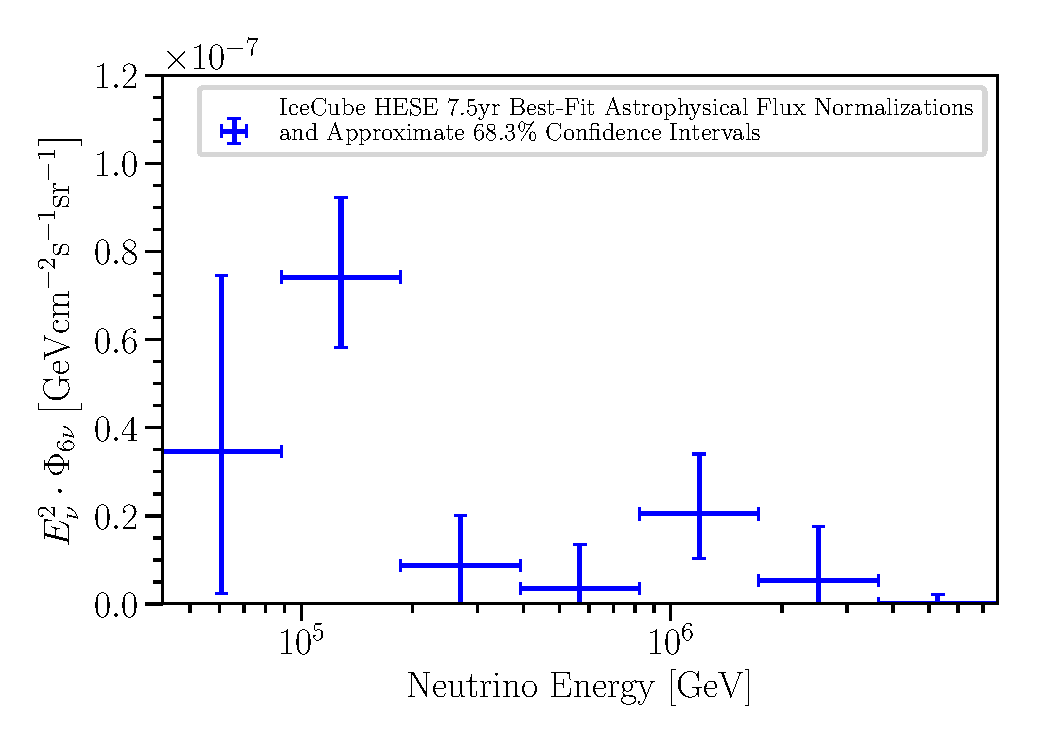
\includegraphics[width=0.45\linewidth]{figures/hese_paper/unfolded_spectrum_freq}
	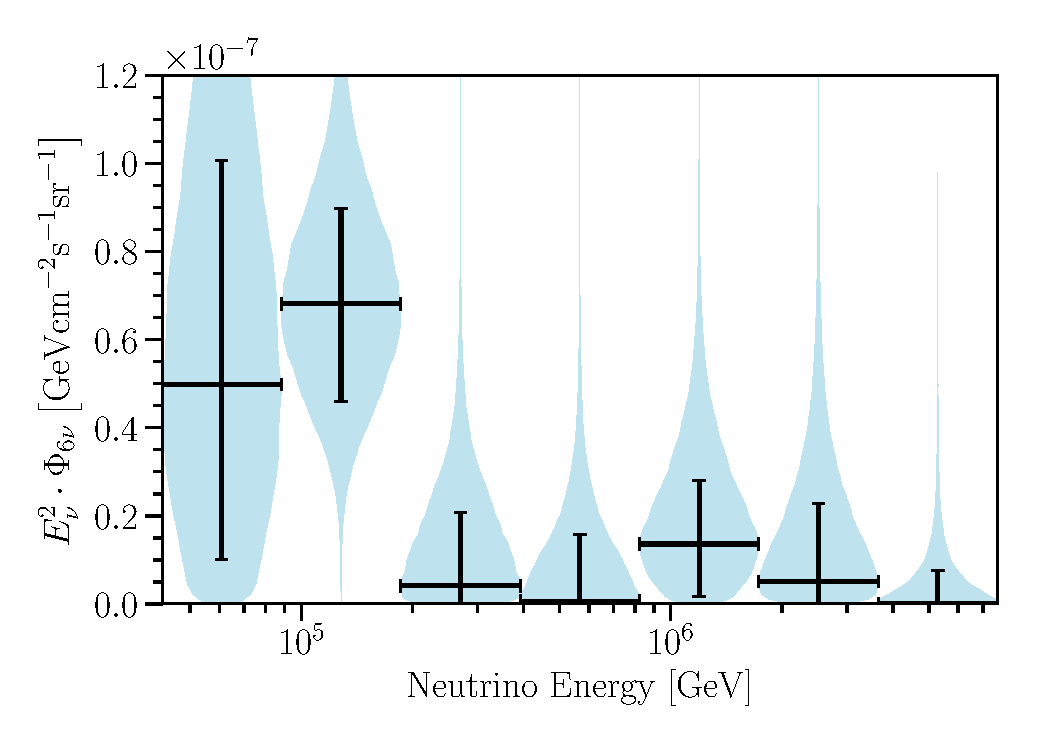
\includegraphics[width=0.45\linewidth]{figures/hese_paper/unfolded_spectrum}
	\internallinenumbers
	\caption{\textbf{\textit{Segmented power-law fit.}}
		The differential flux as obtained by fitting the normalizations of independent $E^{-2}$ segments defined in true neutrino energy.
		Left: in this plot each error bar shows the region in which $\Delta\like\leq0.5$ while holding all other parameters fixed, providing an approximate $\SigmaOne$ confidence level interval for the astrophysical normalization in that particular segment.
		Right: in this plot each error bar shows the $\SigmaOne$ highest probability density credible interval for the astrophysical normalization in that particular segment, assuming a uniform prior on the normalizations.
		The width of the turquoise bands is proportional to the posterior density of the normalization in that segment, and the horizontal scales are arbitrary.}\label{fig:segmented}
\end{figure*}

%\FloatBarrier{}

\subsection{Atmospheric flux from charmed hadrons\label{sec:prompt}}

\noindent
\textit{%Here we discuss the constraints on the flux of neutrinos from the prompt decay of charmed hadrons.
	In this analysis, the astrophysical component and the ``prompt'' neutrino flux can be distinguished by their energy and angular distributions.
	We find no evidence for a prompt component of the atmospheric neutrino flux; normalizations greater than 13 times the baseline model are strongly disfavored with respect to the no-charmed-hadron neutrino flux hypothesis.
	Additionally, we explore an astrophysical flux free hypothesis, and find that this is rejected by more than $5\sigma$ with respect to a single power-law astrophysical plus atmospheric flux hypothesis.
}
\newline

Although most neutrinos in cosmic-ray air showers are produced from the decay of muons, pions, and kaons, at high energies the decay of charmed hadrons can produce neutrinos as well.
Due to the short decay length of charmed hadrons compared to their interaction length, they mostly decay without losing energy, yielding a harder spectrum of neutrinos, compared to the conventional component~\cite{gaisser2016cosmic}, that is more uniform in the zenith angle.
Two ingredients are needed to compute the flux from charmed hadrons: the production cross section of charmed hadrons and the cosmic ray flux.
For this work the relevant part of the production cross section has not been measured at collider experiments as it is only accessible very close to the beam-line where there is little to no instrumentation.
The charmed hadron production cross section can be found by means of perturbative QCD~\cite{Garzelli:2015psa,Gauld:2015kvh,Gauld:2015yia,Bhattacharya:2016jce,Garzelli:2016xmx} and non-perturbative techniques such as dipole-model interactions~\cite{Goncalves:2006ch,Enberg:2008te,Arguelles:2015wba}.
In the region of interest, from $\SI{10}\TeV$ to $\SI{10}\PeV$, the expected flux has an uncertainty of at least a factor of ten in normalization due to parton distribution function and charm mass uncertainties according to~\cite{Garzelli:2016xmx}; though these uncertainty estimations do not include the possibility of additional non-perturbative contributions, {\it e.g.} intrinsic charm~\cite{Laha:2016dri}.
The prompt flux shape variation in this region of interest arises primarily from changes in the cosmic-ray models.
In this analysis we use the BERSS calculation~\cite{Bhattacharya:2016jce} with passing fractions from~\cite{Arguelles:2018awr} as a benchmark prompt flux.

We can perform an analysis of the HESE sample considering only the atmospheric muon and neutrino components.
This results in a best-fit prompt normalization of $\NoAstroPromptNorm$ times the baseline model and is shown in \reffig{fig:prompt_no_astro}.
Another notable point of this background-only fit is that it fails to explain the observed data distribution.
As can be seen from \reffig{fig:prompt_no_astro} the predicted angular distribution fails to explain the southern sky event rate.
Additionally, this value is in tension with constraints on the prompt normalization obtained with the up-going muon neutrino sample~\cite{Aartsen:2013eka,Aartsen:2015rwa,Aartsen:2016xlq}.
Although some of these constraints have been obtained when considering a single-power-law astrophysical component, and are thus dependant on the astrophysical spectral model, the constraints from~\cite{Aartsen:2013eka} predate the observation of high-energy extraterrestrial neutrinos and rely of the lack of high-energy events.
The latter results in a constraint of the prompt normalization of $\ICFiftyNinePromptUpperLimit$ times the ERS calculation~\cite{Enberg:2008te} at $\SI{90}\percent$ C.L.; a model which is approximately $2.5$ times larger than the benchmark model used in this analysis.

\begin{figure*}
	\centering
	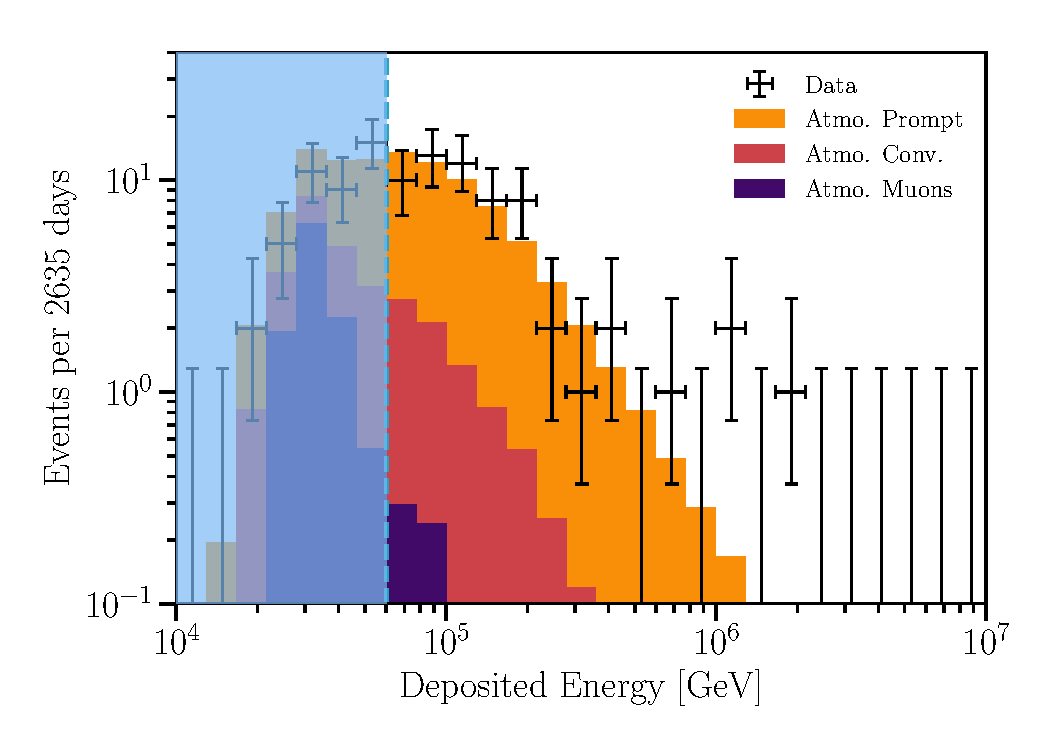
\includegraphics[width=0.45\linewidth]{figures/hese_paper/prompt_only_diffuse_energy_projection_all.pdf}
	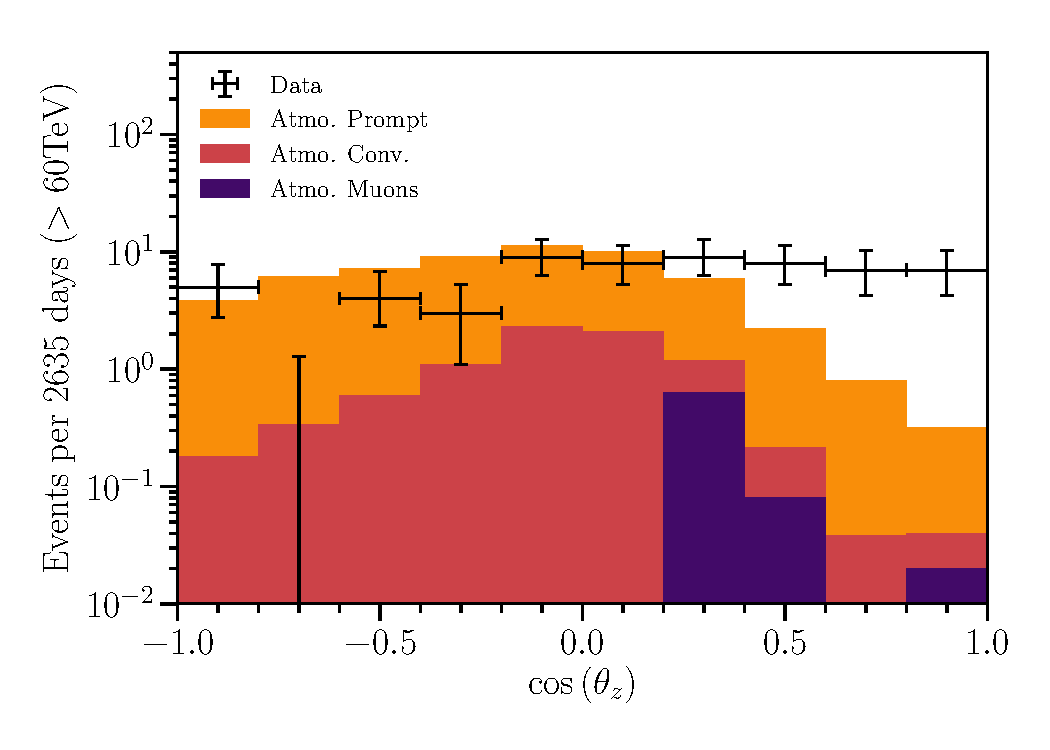
\includegraphics[width=0.45\linewidth]{figures/hese_paper/prompt_only_diffuse_zenith_projection_all.pdf}
	\internallinenumbers
	\caption{\textbf{\textit{Atmospheric-background-only fit to the data.}} In these figures we present the best fit in the absence of an astrophysical component.
		The left panel shows the deposited energy distribution and the right panel the angular distribution.
		As can be seen in the right panel, the angular distribution is in tension with the expectation in several bins.
		This amounts to a greater than $5\sigma$ difference with respect to the best-fit astrophysical model.
		The colors are the same as in \reffig{fig:energy-zenith}.}\label{fig:prompt_no_astro}
\end{figure*}

When we allow for the existence of a single power-law astrophysical component, the best-fit prompt component normalization is zero.
In this same scenario, using the frequentist statistical construction assuming Wilks' theorem with one degree of freedom, a $\SigmaOne$ C.L. prompt normalization upper bound of $\SPLFreqWilksUpperPromptNorm$ and a $\SI{90}\percent$ upper limit of $\SPLFreqWilksNinetyUpperLimit$ is obtained.
This result is in agreement with the results summarized in \reftab{tbl:prompt}.

Additionally, in the Bayesian framework the most-likely value of the prompt normalization is $\SPLBayesPromptNormSummary$ when assuming an improper uniform prior on the prompt normalization.
In this case, the prompt normalization posterior distribution is strongly dependent on the prior choice.
For this reason, we report our Bayesian prompt normalization results in terms of the Bayes factor between the no-prompt hypothesis and a given prompt normalization; see \refsec{sec:statistics} for details.
In \reffig{fig:prompt_bayes} we show the Bayes factor obtained assuming a uniform prior on the astrophysical neutrino normalization and spectral index.
We find that prompt normalizations greater than $\BayesFactorStrongPromptNorm$ are disfavored at the strong level, according to Jeffreys' scale, compared to the no-prompt scenario.

\begin{table*}
	\begin{center}
		\begin{tabular}{l|c| c}
			\hline
			& Frequentist upper limit (90\% C.L.)& Bayesian model rejection (strong) \\
			\hline
			Northern sky muons IC59~\cite{Aartsen:2013eka} & $\ICFiftyNinePromptUpperLimit \times \phi_{ERS}$ & --  \\
			Northern sky muons IC86~\cite{Aartsen:2016xlq} & $1.06 \times \phi_{ERS}$ & -- \\
			All-sky medium-energy starting cascades~\cite{Aartsen:2014muf} & $1.52 \times \phi_{ERS}$ & -- \\
			HESE $\SI{7.5}\year$ (this work) & $\SPLFreqWilksNinetyUpperLimit \times \phi_{BERSS}$ & $ 13.21 \times \phi_{BERSS}$ \\
			\hline
		\end{tabular}
	\end{center}
	\internallinenumbers
	\caption{\textit{\textbf{Summary of constraints on the flux of charmed mesons.}} The benchmark $\phi_{ERS}$~\cite{Enberg:2008te} and $\phi_{BERSS}$~\cite{Bhattacharya:2016jce}, are such that $\phi_{ERS}(\SI{100}\TeV) \approx 2.5 \cdot \phi_{BERSS}(\SI{100}\TeV)$.}
	\label{tbl:prompt}
\end{table*}

\begin{figure}
	\centering
	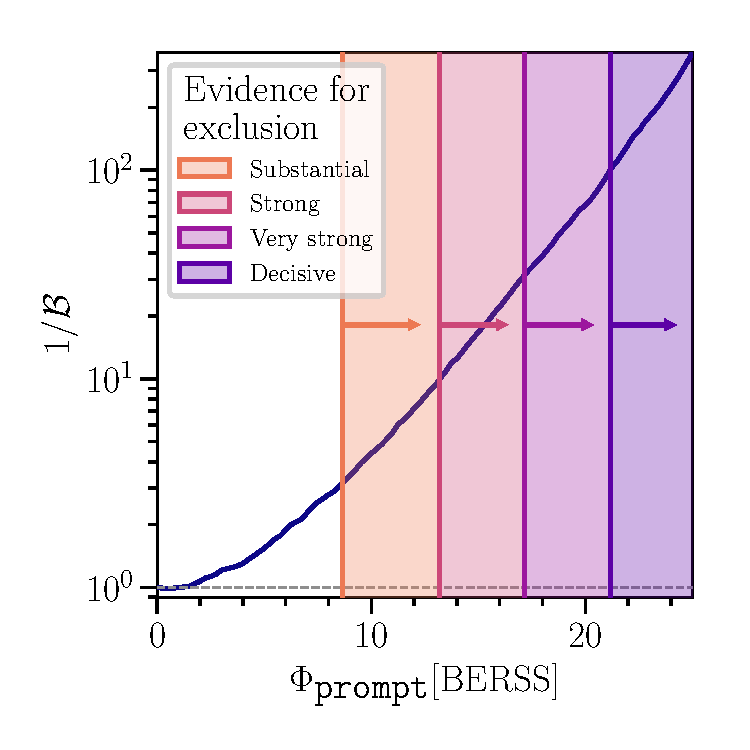
\includegraphics[width=\linewidth]{figures/hese_paper/prompt_bayes}
	\internallinenumbers
	\caption{\textbf{\textit{Prompt neutrino normalization constraints.}}
		The horizontal axis shows the size of the prompt normalization with respect to the baseline BERSS model discussed in \refsec{sec:backgrounds} with passing fractions given in~\cite{Arguelles:2018awr}.
		The vertical axis gives the reciprocal of the Bayes factor; decreasing Bayes factors imply a more disfavored prompt normalization.
		The shaded regions denote exclusions of the prompt normalization according to Jeffreys' scale from substantial to decisive.}\label{fig:prompt_bayes}
\end{figure}

\subsection{Source-specific models\label{sec:specific_models}}

\noindent
\textit{We selected a number of models from the literature that predict the neutrino flux from a variety of sources (AGN, low-luminosity AGN BLLacs, choked jets in core-collapse SN, star burst galaxies, low-luminosity BLLacs, and GRBs).
	We tested these models against a baseline single power-law astrophysical flux model by considering two types of alternative hypotheses.
	The first where a source model comprises the entire neutrino flux; the second where a source model and a single power law both contribute to the flux.
	None of these alternative scenarios are strongly favored compared to the single power-law hypothesis.
	Of the models tested some are disfavored with the benchmark values of their parameters, see \reftab{tbl:diffuse_models} for more information.
}
\newline

In \refsec{sec:generic_models} we characterized the observed astrophysical neutrino events by means of generic models.
These studies show that a single power law is a good fit to the data.
Nevertheless, in this section we study the compatibility of the observed events with specific source predictions of the astrophysical neutrino flux proposed in the literature.
The models used in this analysis together with the result of the segmented power-law fit can be seen in \reffig{fig:source_models_fluxes}.
The models we consider are such that they have significant flux contribution in the energy range that this analysis is sensitive to.
Thus, {\it e.g.} we do not test cosmogenic~\cite{Halzen:1992cz} neutrino flux models, which predict neutrinos from cosmic rays interacting with the cosmic microwave background, since they are expected to contribute at higher energies where dedicated IceCube searches exist~\cite{Aartsen:2018vtx}; see~\cite{Safa:2019ege} for a recent discussion on the expected rate of cosmogenic flux in this analysis energy range.

Astrophysical neutrino flux predictions have in principle many parameters that may modify the expected flux.
For simplicity, in this analysis, we do not study the internal parameters of the models but limit ourselves to some nominal values of their parameters.
The analysis takes the form of a model selection test with two non-nested equally likely alternatives.

In our primary analysis, the two alternatives are: a single power law and a source model.
Our model comparison test uses the Bayes factor of these two models as a criterion for model selection; see \refsec{sec:statistics} for details.
Thus the single power law serves as a benchmark model to compare against.
In the case of the single power-law model we calculate the evidence by marginalizing over the two model parameters, normalization and spectral index, assuming uniform priors in a compact region defined as $(\astronorm,\astrodeltagamma) \in [0, 25]\times [2,4]$, as well as the analysis nuisance parameters with priors given in \reftab{tbl:priors}.
The alternative source model has no free parameters and thus the evidence integral is only over the nuisance parameters.
In \reffig{fig:source_models_fluxes} we show the models with a color scale that orders models by their evidence.
In this study, the single power law is penalized due to additional model complexity with respect to the source model.

\begin{table*}
	\centering
	\begin{minipage}{\linewidth}
		\begin{tabular}{l l r r r r}
			\toprule
			\multirow{2}{*}{\makecell[l]{}Source class} & \multirow{2}{*}{\makecell[l]{Model}} & \multirowcell{2}{Model only \\ Bayes factor} & \multirowcell{2}{Model + SPL \\ Bayes factor} & \multirowcell{2}{Most-likely \\ SPL $\astrodeltagamma$} & \multirowcell{2}{Most-likely \\ SPL $\astronorm$} \\
			& & & & & \\ \midrule
			%\SPLTableSummary \\ \midrule
			%\DPLTableSummary \\ \midrule
			%\LPTableSummary \\ \midrule
			\SteckerTableSummary \\ \midrule
			\FangTableSummary \\ \midrule
			\KimuraBOneTableSummary \\ \midrule
			\KimuraBFourTableSummary \\ \midrule
			\KimuraTwoCompTableSummary \\ \midrule
			\MariaBLLacsTableSummary \\ \midrule
			\MurasechockedJetsTableSummary \\ \midrule
			\SBGminBmodelTableSummary \\ \midrule
			\TavecchilowPowerTableSummary \\ \midrule
			\TDEWinterBiehlTableSummary \\ \midrule
			\bottomrule
		\end{tabular}
	\end{minipage}
	\begin{minipage}{\linewidth}
		\internallinenumbers
		\caption{\textbf{\textit{Astrophysical neutrino flux model comparison test results.}} Each row shows the source-specific model tested, the Bayes factor of the model on its own, the Bayes factor of the model in conjunction with a power-law component, the most likely spectral index of the accompanying power-law component with corresponding $\SigmaOne$ HPD region, and the most likely normalization of the accompanying power-law component with corresponding $\SigmaOne$ HPD region.} \vspace{-6mm}\label{tbl:diffuse_models}
	\end{minipage}
\end{table*}

Since some models, in the literature, are not intended to explain the whole astrophysical neutrino spectrum a secondary analysis is also performed.
In this analysis we consider two models: a single power law on its own and a single power law together with a source model.
In this case, the constant parameter-space factor of the single power-law flux parameters compact region cancel and so we are able to use improper uniform priors without introducing an arbitrary scaling factor.
The same prior dependence that is in the other Baeysian analyses still remains, as the likeloods of the two models can peak in different regions of parameter space.

The results of both analyses are shown in \reftab{tbl:diffuse_models}.
For each model we report the ``Model only Bayes factor'' as the result of the primary analysis and for the secondary analysis we report the ``Model plus single power-law Bayes factor'' together with the most-likely spectral index and normalization of the accompanying power law; the 68.3\% parameter HPD intervals are also reported.

\begin{figure*}
	\centering
	\subfloat{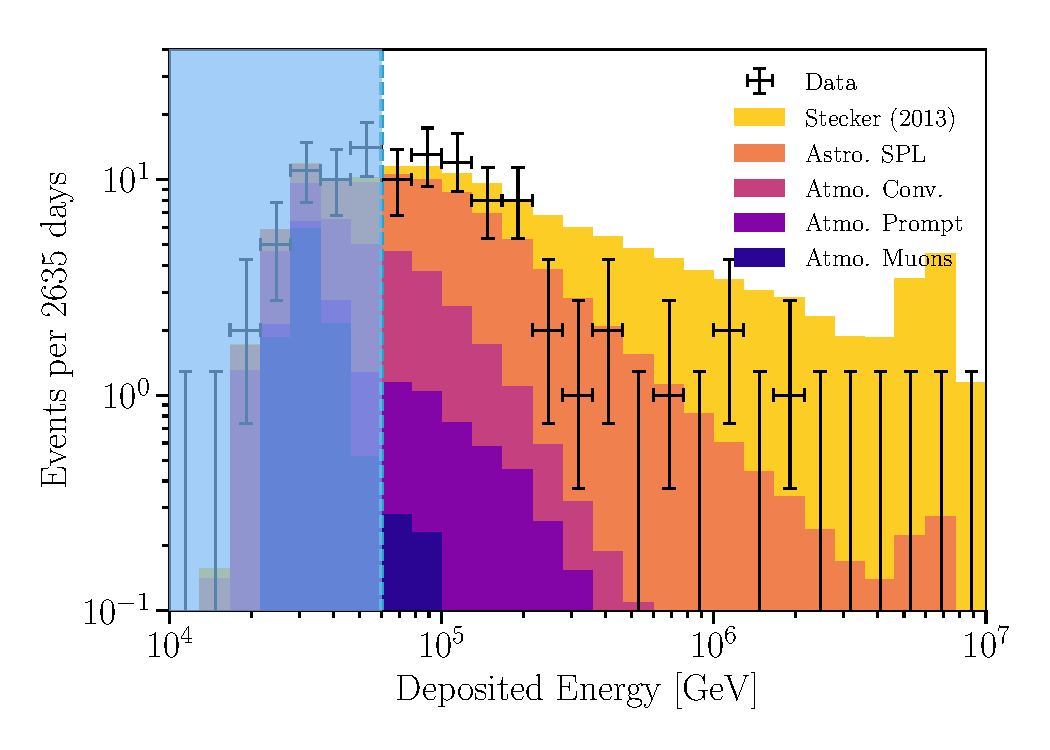
\includegraphics[width=0.45\linewidth]{figures/hese_paper/diffuse_energy_projection_all_stecker_agn}}
	\subfloat{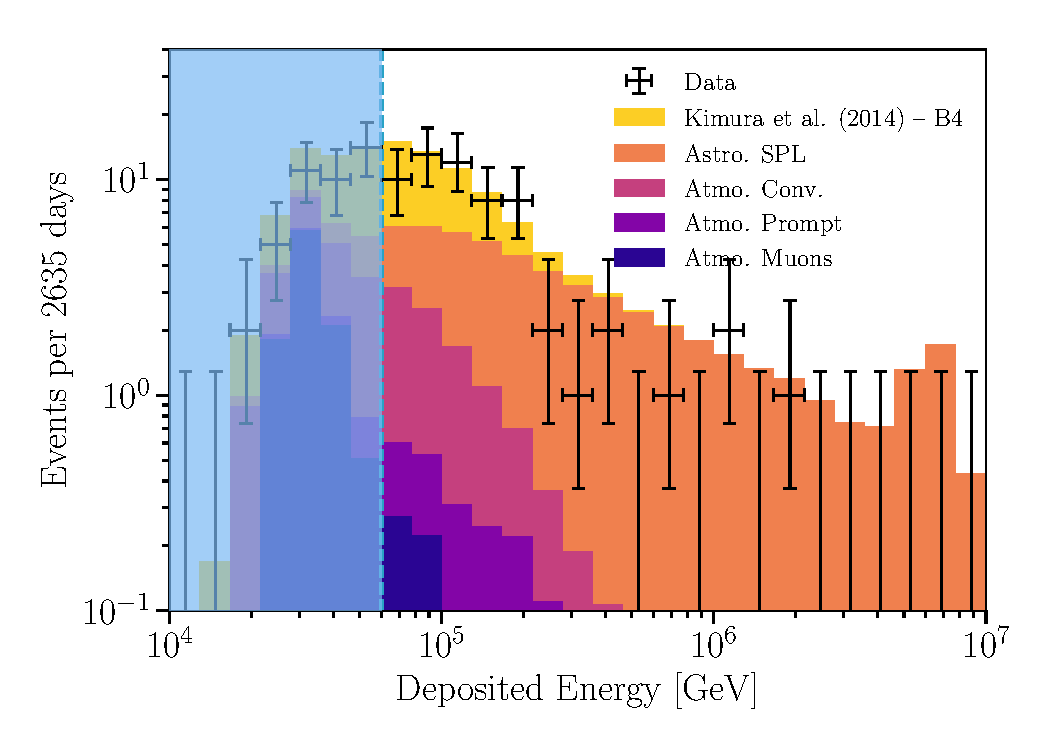
\includegraphics[width=0.45\linewidth]{figures/hese_paper/diffuse_energy_projection_all_LLGAGN_modelB4}}
	\internallinenumbers
	\caption{\textbf{\textit{Source-specific model energy distributions.}}
		Different panels show the predicted energy distribution compare to the data for a subset of the models consider in \reftab{tbl:diffuse_models}.
		In all of these cases we have added an additional single power-law component.
		All the components are shown as a stacked histogram at the most likely value of the background components normalizations.
		Left: \Stecker~model as an example as an example of case where the Bayes factor indicates significant preference of the single power law.
		Right: \KimuraBFour~model as an example of case where an additional single power law is needed to explain the distribution.}\label{fig:source_models}
\end{figure*}

Given the obtained Bayes factors models can be organized into two categories:
\begin{itemize}
	\item Models with Bayes factors much less than one for both analyses.
	In this case, the single power law is a better description of the data and the addition of an additional single power law to the source model does not alter this conclusion.
	See \reffig{fig:source_models} (left) for an example of this category.
	\item Models with Bayes factor much less than one when compared to the single power law, but that are favored when introducing an additional single power-law component.
	Models in this category are only able to describe part of the flux, and would require the existence of a second component to be compatible with the data.
	See \reffig{fig:source_models} (right) for an example of this category.
	%\item Models with Bayes factors much larger than one, are thus preferred by the data with respect to the single power-law generic model.
	%For these models, adding an additional single power-law component can reduce the total model evidence due to increased model complexity.
	%See \reffig{fig:source_models} (right) for an example of this category.
\end{itemize}
To conclude, in this section we have studied models of astrophysical neutrinos proposed in the literature and compare them to the our baseline generic parameterization, the single power-law spectrum.
We find that no model is substantially preferred over the baseline model, and some models -- those with Bayes factors much smaller than unity -- are disfavored; see \reftab{tbl:diffuse_models}.

\begin{figure}
	\centering
	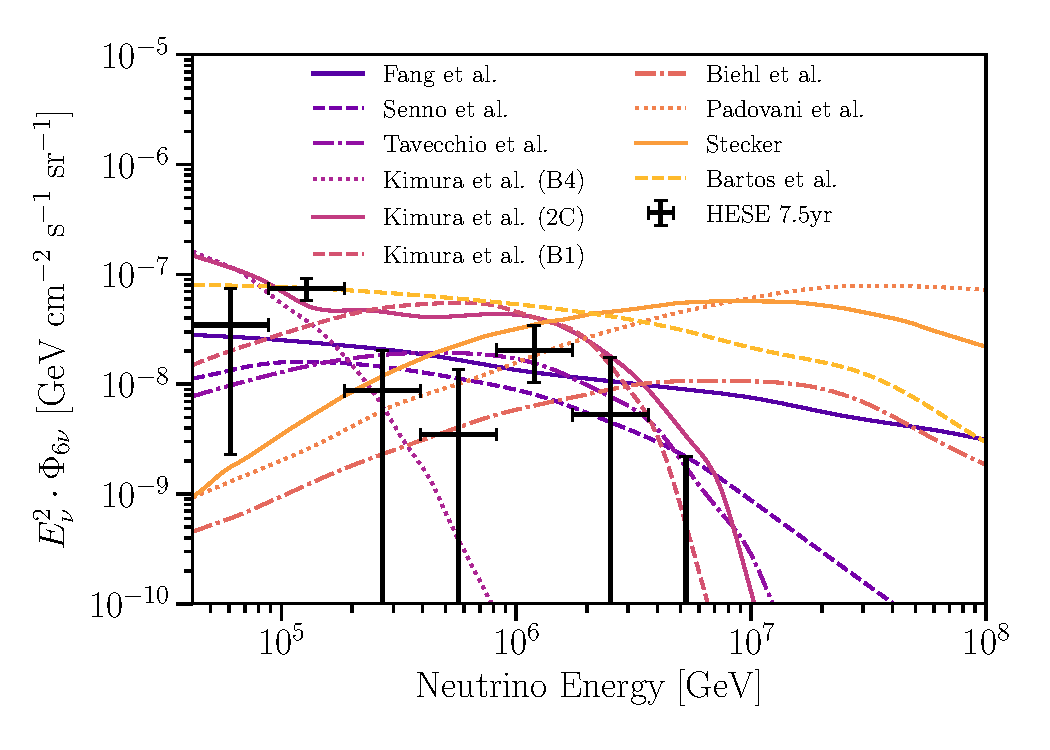
\includegraphics[width=\linewidth]{figures/hese_paper/HESE_flux_with_ad_hoc_models}
	\internallinenumbers
	\caption{\textbf{\textit{Source-specific models tested in this work together with the segmented-fit outcome.}}
		Models discussed in \refsec{sec:specific_models} and listed in \reftab{tbl:diffuse_models} are shown as lines.
		The HESE segmented power-law model, described in \refsec{sec:unfolding}, best-fit normalizations are shown as black crosses.
		Models are ordered in the color scale from largest (darkest color) to smallest (lightest color) evidence as reported in \reftab{tbl:diffuse_models}.}
	\label{fig:source_models_fluxes}
\end{figure}

